\part{基础∞-范畴论}
\chapter{∞-宇宙及其同伦 2-范畴}\label{ch:infinity-cosmoi}

在本章中，我们引入一套框架，以发展\trInfinityCategory{}的\trFormal{}范畴理论；
这套框架名为\emph{\trInfinityCosmos}。非正式地说，一个\trInfinityCosmos{}是一个
$(\infty,2)$-范畴——即一个富集于 $(\infty,1)$-\trCategory{}之上的\trCategory{}——
并配备有 $(\infty,2)$-范畴论极限。在诸\trInfinityCosmos{}的动机性例子中，
其对象是某一模型中的\trInfinityCategory。为使这套抽象理论紧扣其预期的解读，
我们把「∞-范畴」重新设定为一个技术性术语，专指任一周围\trInfinityCosmos{}中的对象。

出人意料的是，这些动机性例子使我们得以对「配备 $(\infty,2)$-范畴论极限的
$(\infty,2)$-范畴」一语作相当严格的解读：一个\trInfinityCosmos{}是一种特殊类型的%
\trSimpliciallyEnrichedCategory{}，而这些 $(\infty,2)$-范畴论极限则以%
\trSimpliciallyEnrichedLimit{}为模型。更精确地说，一个\trInfinityCosmos{}是一个
富集于\trQuasiCategory{}之上的\trCategory{}，而\trQuasiCategory{}本身即是把
$(\infty,1)$-范畴定义为特定\trSimplicialSet{}的诸模型之一。这些 $(\infty,2)$-范畴论极限
被定义为「涉及一类名为\emph{\trIsofibration}的指定映射」的图表之\trLimit{}——
这类映射并无内在的\trHomotopy{}意义，因为\trInfinityCategory{}之间的任何%
\trFunctor{}都\trEquivalence{}于一个\trIsofibration{}——但它们使我们得以考虑
严格交换的图表。

在 §1.1 中，我们引入\trQuasiCategory{}，回顾那些为证明\trQuasiCategory{}自身
能够构成一个\trInfinityCosmos{}——即原型性的例子——所需的经典结果。
一般的\trInfinityCosmos{}在 §1.2 中定义，该节给出若干例子并确立其基本性质。
在 §1.3 中，我们转向\trInfinityCosmos{}之间的\emph{\trCosmologicalFunctor}，
后者保持全部的定义性结构。\trCosmologicalFunctor{}有双重用途：一方面
在许多证明中提供技术上的简化，其后又充当确立\trInfinityCategory{}理论%
\trModelIndependence{}的「\trChangeOfModel{}」\trFunctor。

最后，在 §1.4 中，我们引入一个严格的 2-范畴：其对象是\trInfinityCategory{}，
其 1-\trCell{}是其间的 ∞-\trFunctor{}，而其 2-\trCell{}则定义这些%
\trFunctor{}之间的\trInfinityNaturalTransformation。任何\trInfinityCosmos{}%
都有这样一个 2-范畴，我们称之为该\trInfinityCosmos{}的\trHomotopyTwoCategory。
事实上，急于看到\trInfinityCategory{}的范畴理论得到发展的读者，初读时
可以跳过本章，把\trHomotopyTwoCategory{}的存在性视为理所当然，
而直接从第 2 章开始。

\newcommand{\qcOne}{\mathbf{1}}   %
\newcommand{\qcTwo}{\mathbf{2}}   %
\newcommand{\qcThree}{\mathbf{3}} %
\newcommand{\qcN}{\mathbf{n}}     %
\newcommand{\qcInt}{\mathbb{I}}   %
\newcommand{\qcEquiv}{\rightsquigarrow}                 %
\newcommand{\qcTFib}{\overset{\wr}{\twoheadrightarrow}} %

\section{\trQuasiCategory}\label{sec:quasi-categories}

在引入一套公理化框架、以便一般地发展 \trInfinityCategory{}理论之前，
我们先专门考察一个模型：\textbf{\trQuasiCategory}（quasi-category）——
它由 Boardman 与 Vogt 在其\trHomotopy{}相干图（homotopy coherent diagram）研究中
于 1973 年引入\cite{bib21}。通常的 1-\trCategory{}经由\cref{def:nerve}的构造给出%
\trQuasiCategory{}的例子。Joyal 在\cite{bib61}与\cite{bib63}以及若干未出版的书稿
草稿中率先承担起把 1-\trCategory{}理论\trExtension{}为\trQuasiCategory{}理论的任务；本节的大多数结果
都归功于他。

\begin{notation}[\trSimplexCategory]\label{not:simplex-category}
记 $\Delta$ 为由有限非空序数 $[n]=\{0<1<\cdots<n\}$ 及保序映射构成的
\textbf{\trSimplexCategory}（simplex category）。其中特别包括
\[
\begin{array}{ccccc}
\text{初等\trFaceOperator} & [n-1] & \xrightarrow{\;\delta^i\;} & [n] & 0\le i\le n\\
\text{初等\trDegeneracyOperator} & [n+1] & \xrightarrow{\;\sigma^i\;} & [n] & 0\le i\le n
\end{array}
\]
其像分别在元素 $i\in[n]$ 处略去、重复该元素。$\Delta$ 中每个态射都唯一地
分解为一个\trEpimorphism{}后接一个\trMonomorphism{}；这些\trEpimorphism{}即\textbf{\trDegeneracyOperator}
（degeneracy operator），可分解为初等\trDegeneracyOperator{}的复合；而\trMonomorphism{}即
\textbf{\trFaceOperator}（face operator），可分解为初等\trFaceOperator{}的复合。
\end{notation}

\textbf{\trSimplicialSet}（simplicial set）的\trCategory{}是\trSimplexCategory{}上预层
（presheaf）的\trCategory{}，记作
$s\mathcal{S}et\coloneqq\mathcal{S}et^{\Delta^{\mathrm{op}}}$。
我们以 $\Delta[n]$ 记\textbf{标准 $n$-\trSimplex}（standard $n$-simplex），
即由 $[n]\in\Delta$ 所表示的\trSimplicialSet{}；并以
$\Lambda^k[n]\subset\partial\Delta[n]\subset\Delta[n]$ 记它的
\textbf{$k$-\trHorn}（$k$-horn）与\textbf{\trBoundarySphere}（boundary sphere）。
\yizhu{horn 直译为「角」；本译取「\trHorn」，以便「内\trHorn」「外\trHorn」
「左外\trHorn」等复合词读感统一。}球面 $\partial\Delta[n]$ 是由 $n$-\trSimplex{}余维数
为一的诸面生成的单纯子集，而\trHorn $\Lambda^k[n]$ 是再略去顶点 $k$
对面的那个面所得的单纯子集。

给定\trSimplicialSet $X$，习惯上以 $X_n$ 记它的 $n$-\trSimplex{}之集，即在 $[n]\in\Delta$
处取值所得。由\trYonedaLemma{}，每个 $n$-\trSimplex{} $x\in X_n$ 对应一个\trSimplicialSet
映射 $x\colon\Delta[n]\to X$。相应地，记 $x\cdot\delta^i$ 为该 $n$-\trSimplex{}的
第 $i$ 个面，即由复合映射
\[
\Delta[n-1]\xrightarrow{\;\delta^i\;}\Delta[n]\xrightarrow{\;x\;}X
\]
分类的 $(n-1)$-单纯形。\trFaceOperator{}的右作用定义了映射
$X_n\xrightarrow{\;\cdot\delta^i\;}X_{n-1}$。几何上，$x\cdot\delta^i$
就是 $n$-\trSimplex{} $x$ 中「顶点 $i$ 对面的面」。

\begin{definition}[\trQuasiCategory]\label{def:quasi-category}
\trQuasiCategory{}是一个\trSimplicialSet $A$，其中任何\textbf{内\trHorn}
（inner horn）都能\trExtension{}为\trSimplex{}，即求解图示的\trLifting{}问题（lifting problem）：
\begin{rveq}\label{eq:inner-horn-lifting}
\mbox{\begin{tikzpicture}[x=1.5em,y=1.5em]
  \node (tl) at (0,1.3) {$\Lambda^k[n]$};
  \node (tr) at (3.0,1.3) {$A$};
  \node (bl) at (0,0) {$\Delta[n]$};
  \draw[->] (tl) -- (tr);
  \draw[->] (0,0.95) -- (0,0.3);
  \draw (0,0.95) arc[start angle=180,end angle=0,radius=0.16];
  \draw[->,dashed] (0.45,0.2) -- (2.7,1.15);
  \node at (8.3,0.65) {对 $n\ge 2$，$0<k<n$。};
\end{tikzpicture}}
\end{rveq}
\end{definition}

\trQuasiCategory{}由 Boardman 与 Vogt 首次引入\cite{bib21}，当时称作「弱\trKanComplex」——
\textbf{\trKanComplex}（Kan complex）指沿一切\trHorn{}包含 $n\ge 1$，$0\le k\le n$
都能给出如\eqref{eq:inner-horn-lifting}那样的\trExtension{}的\trSimplicialSet{}。
由于任何拓扑空间都能编码为\trKanComplex{}，\footnote{总奇异复形（total singular
complex）构造定义了从拓扑空间到\trSimplicialSet{}的一个\trFunctor{}，它在两者的\trHomotopyCategory{}上是%
\trEquivalence{}：空间的弱\trHomotopy{}型对应\trKanComplex{}的\trHomotopy\trEquivalence{}类\cite{bib93}。由
\cref{ex:nerve-cosimplicial}构造的左\trAdjunction{}则把\trSimplicialSet{}「几何实现」为一个
拓扑空间。}空间便以此方式给出\trQuasiCategory{}的例子。

\trCategory{}也经由\trNerve{}（nerve）构造给出\trQuasiCategory{}的例子。

\begin{definition}[\trNerve]\label{def:nerve}
1-\trCategory{}的\trCategory $\mathcal{C}at$ 经由\textbf{\trNerve{}函子}（nerve functor）
\trFullyFaithful{}嵌入\trSimplicialSet{}的\trCategory{}。1-\trCategory $C$ 的\trNerve{}中的 $n$-单纯形是 $C$ 中
$n$ 个可合成箭头的序列，\trEquivalence{}地，是一个从\trOrdinalCategory{}（ordinal category）
$\qcN+\qcOne\coloneqq[n]$ 到 $C$ 的\trFunctor——该\trCategory{}有对象
$0,\ldots,n$，并且恰在 $i\le j$ 时才有唯一箭头 $i\to j$。
\end{definition}

映射 $[n]\mapsto\qcN+\qcOne$ 定义了一个\trFullyFaithful{}嵌入
$\Delta\hookrightarrow\mathcal{C}at$。从这个观点看，\trNerve{}函子可以描述为
一部「限制的\trYonedaEmbedding」：它把\trCategory{} $C$ 送到可表示\trFunctor
$\mathrm{hom}(-,C)$ 在这一包含的像上的限制。更一般的「\trNerve{}型构造」见
\cref{ex:nerve-cosimplicial}。

\begin{remark}\label{rem:nerve-2-coskeletal}
\trCategory{} $C$ 的\trNerve{}作为\trSimplicialSet{}是\textbf{\trTwoCoskeletal}（2-coskeletal），
意即每个 $n\ge 3$ 的球面 $\partial\Delta[n]\to C$ 都由 $C$ 中某个
$n$-\trSimplex{}唯一填充（见定义 C.5.2）。%
注意：球面 $\partial\Delta[2]\to C$ 能\trExtension{}成一个 2-\trSimplex{}，当且仅当沿其对角
边的箭头是内\trHorn $\Lambda^1[2]\subset\partial\Delta[2]\to C$ 中沿诸边的
那些箭头的复合。维数 3 及以上的\trSimplex{}则见证：沿其\textbf{\trSpine}（spine）——
由连接相邻顶点的边组成的 1-骨架单纯子集——的可合成箭头路径，其合成满足
结合律。事实上，正如\cref{prop:nerves-quasi-categories}的证明所提示的，
任何内\trHorn{}都有\emph{唯一}\trFiller{}的\trSimplicialSet{}都\trIsomorphism{}于某个 1-\trCategory{}的\trNerve
（见\cref{ex:unique-fillers}）。
\end{remark}

我们不愿为\trNerve{}函子引入显式记号，而更愿意把 1-\trCategory{}与它们的\trNerve{}等同起来。
我们将发现：1-\trCategory{}的理论可以这样\trExtension{}到以\trQuasiCategory{}为模型的%
\trInfinityCategory{}上，使得每个 \trInfinityCategory{}概念沿\trNerve{}嵌入的限制都恢复出
相应的 1-\trCategory{}概念。例如，标准单纯形 $\Delta[n]$ \trIsomorphism{}于\trOrdinalCategory
$\qcN+1$ 的\trNerve{}，于是我们时常采用后一种记号——写
$\qcOne\coloneqq\Delta[0]$，$\qcTwo\coloneqq\Delta[1]$，$\qcThree\coloneqq\Delta[2]$，
如此等等——以暗示正确的\trCategory{}直觉。\yizhu{原书以空心数字
$\qcOne$、$\qcTwo$、$\qcThree$ 分别记 $\Delta[0]$、$\Delta[1]$、$\Delta[2]$；
译本以粗体数字近似排印。}

要沿这条路走下去，必须先核实刚刚隐含作出的那个断言：

\begin{proposition}[\trNerve{}是\trQuasiCategory]\label{prop:nerves-quasi-categories}
\trCategory{}的\trNerve{}是\trQuasiCategory{}。
\end{proposition}
\begin{proof}
经由\cref{rem:nerve-2-coskeletal}中的\trIsomorphism $C\cong\mathrm{cosk}_2\,C$
与 C.5.2 中的\trAdjunction{} $\mathrm{sk}_2\dashv\mathrm{cosk}_2$，
下方左侧所示的\trLifting{}问题转置为右侧所示者：
\begin{center}
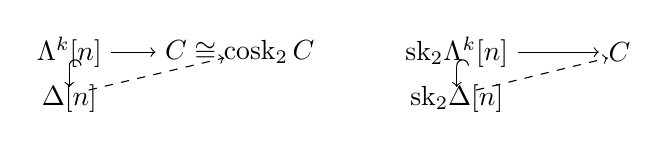
\begin{tikzpicture}[x=1.4em,y=1.4em]
  \node (tl) at (0,1.2) {$\Lambda^k[n]$};
  \node (tr) at (4.4,1.2) {$C\cong\mathrm{cosk}_2\,C$};
  \node (bl) at (0,0) {$\Delta[n]$};
  \draw[->] (tl) -- (tr);
  \draw[->] (0,0.85) -- (0,0.3);
  \draw (0,0.85) arc[start angle=180,end angle=0,radius=0.15];
  \draw[->,dashed] (0.5,0.22) -- (4.0,1.05);
  \node at (7.2,0.6) {$\leftrightsquigarrow$};
  \node (tl2) at (10.0,1.2) {$\mathrm{sk}_2\Lambda^k[n]$};
  \node (tr2) at (14.2,1.2) {$C$};
  \node (bl2) at (10.0,0) {$\mathrm{sk}_2\Delta[n]$};
  \draw[->] (tl2) -- (tr2);
  \draw[->] (10.0,0.85) -- (10.0,0.3);
  \draw (10.0,0.85) arc[start angle=180,end angle=0,radius=0.15];
  \draw[->,dashed] (10.5,0.22) -- (13.9,1.05);
\end{tikzpicture}
\end{center}
\trFunctor{} $\mathrm{sk}_2$ 把\trSimplicialSet{}替换成它的\textbf{2-\trSkeleton}
（2-skeleton）：由维数至多 2 的\trSimplex{}生成的单纯子集。
当 $n\ge 4$ 时，
包含 $\mathrm{sk}_2\Lambda^k[n]\hookrightarrow\mathrm{sk}_2\Delta[n]$
是\trIsomorphism{}，此时右侧的\trLifting{}问题有（唯一的）解。于是只剩下 $n=2$ 与 $n=3$
两种情形需要求解左侧的\trLifting{}问题。为此考察
\begin{center}
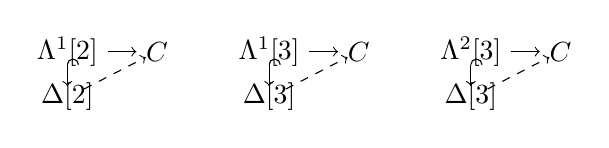
\begin{tikzpicture}[x=1.35em,y=1.35em]
  \node (a1) at (0,1.2) {$\Lambda^1[2]$};
  \node (a2) at (2.4,1.2) {$C$};
  \node (a3) at (0,0) {$\Delta[2]$};
  \draw[->] (a1) -- (a2);
  \draw[->] (0,0.85) -- (0,0.28);
  \draw (0,0.85) arc[start angle=180,end angle=0,radius=0.15];
  \draw[->,dashed] (0.45,0.2) -- (2.1,1.05);
  \node (b1) at (5.4,1.2) {$\Lambda^1[3]$};
  \node (b2) at (7.8,1.2) {$C$};
  \node (b3) at (5.4,0) {$\Delta[3]$};
  \draw[->] (b1) -- (b2);
  \draw[->] (5.4,0.85) -- (5.4,0.28);
  \draw (5.4,0.85) arc[start angle=180,end angle=0,radius=0.15];
  \draw[->,dashed] (5.85,0.2) -- (7.5,1.05);
  \node (c1) at (10.8,1.2) {$\Lambda^2[3]$};
  \node (c2) at (13.2,1.2) {$C$};
  \node (c3) at (10.8,0) {$\Delta[3]$};
  \draw[->] (c1) -- (c2);
  \draw[->] (10.8,0.85) -- (10.8,0.28);
  \draw (10.8,0.85) arc[start angle=180,end angle=0,radius=0.15];
  \draw[->,dashed] (11.25,0.2) -- (12.9,1.05);
\end{tikzpicture}
\end{center}
内\trHorn $\Lambda^1[2]\to C$ 给出 $C$ 中一个可合成箭头对；之所以存在到
2-\trSimplex{}的\trExtension{}，正因为任何可合成箭头对都有（唯一的）合成。

内\trHorn $\Lambda^1[3]\to C$ 给出 $C$ 中三个可合成箭头的数据——如下图所示——
连同复合 $gf$、$hg$ 与 $(hg)f$。
\begin{center}
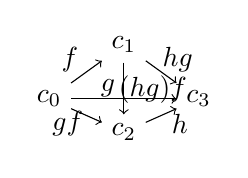
\begin{tikzpicture}[x=1.5em,y=1.5em]
  \node (c0) at (0,0.8) {$c_0$};
  \node (c1) at (1.8,2.1) {$c_1$};
  \node (c2) at (1.8,0) {$c_2$};
  \node (c3) at (3.6,0.8) {$c_3$};
  \draw[->] (c0) -- (c1);
  \node at (0.5,1.75) {$f$};
  \draw[->] (c1) -- (c3);
  \node at (3.1,1.75) {$hg$};
  \draw[->] (c0) -- (c3);
  \node at (2.5,1.02) {$(hg)f$};
  \draw[->] (c0) -- (c2);
  \node at (0.45,0.2) {$gf$};
  \draw[->] (c2) -- (c3);
  \node at (3.15,0.2) {$h$};
  \draw[->] (c1) -- (c2);
  \node at (1.42,1.05) {$g$};
\end{tikzpicture}
\end{center}
由于合成满足结合律，箭头 $(hg)f$ 同样是 $gf$ 接 $h$ 的复合，这就证得
顶点 $c_1$ 对面的 2-\trSimplex{}存在于 $C$ 中；再由 2-余骨架性，填充这一边界
球面的 3-\trSimplex{}也存在于 $C$ 中。\trHorn $\Lambda^2[3]\to C$ 的\trFiller{}可
类似地构造。
\end{proof}

\begin{definition}[1-\trSimplex{}上的\trHomotopyRelation]\label{def:homotopy-1-simplices}
\trSimplicialSet $X$ 中平行的 1-\trSimplex{} $f$ 与 $g$ 称为\textbf{\trHomotopy{}的}
（homotopic），若存在一个 2-\trSimplex{}，其边界取下列两种形状之一，
\footnote{记号「═」在图中表示一个退化单纯形或恒等箭头。}
\begin{rveq}\label{eq:homotopic-forms}
\mbox{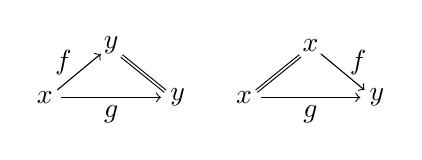
\begin{tikzpicture}[x=1.5em,y=1.5em]
  \node (x1) at (0,0) {$x$};
  \node (y1) at (1.6,1.25) {$y$};
  \node (y2) at (3.2,0) {$y$};
  \draw[->] (0.3,0.18) -- (1.35,1.05);
  \node at (0.45,0.85) {$f$};
  \draw[double] (1.85,1.0) -- (2.9,0.15);
  \draw[->] (0.4,0) -- (2.8,0);
  \node at (1.6,-0.4) {$g$};
  \node (x3) at (6.4,1.25) {$x$};
  \node (x4) at (4.8,0) {$x$};
  \node (y3) at (8.0,0) {$y$};
  \draw[double] (5.1,0.15) -- (6.15,1.0);
  \draw[->] (6.65,1.05) -- (7.7,0.18);
  \node at (7.55,0.85) {$f$};
  \draw[->] (5.2,0) -- (7.6,0);
  \node at (6.4,-0.4) {$g$};
\end{tikzpicture}}
\end{rveq}
或者 $f$ 与 $g$ 落在这一关系所生成的同一个\trEquivalence{}类里。
\end{definition}

在\trQuasiCategory{}中，由\eqref{eq:homotopic-forms}所展示的任一类型的 2-\trSimplex{}所
见证的关系都是\trEquivalence{}关系，而且这两种\trEquivalence{}关系重合。

\begin{lemma}[\trQuasiCategory{}中\trHomotopy{}的 1-\trSimplex]\label{lem:homotopic-quasi-category}
\trQuasiCategory{}中平行的 1-\trSimplex{} $f$ 与 $g$ 是\trHomotopy{}的，当且仅当存在一个
\eqref{eq:homotopic-forms}所示任一形状——\trEquivalence{}地，所有形状——的
2-\trSimplex{}。
\end{lemma}
\begin{proof}
见\cref{ex:homotopy-equivalence}。
\end{proof}

\begin{definition}[\trHomotopyCategory{}；\cite{bib44}~\S2.4]\label{def:homotopy-category}
经 1-截断，任何\trSimplicialSet $X$ 都带有底层的\textbf{\trReflexiveDirectedGraph}
（reflexive directed graph）：$X$ 的 0-\trSimplex{}定义对象，1-\trSimplex{}定义箭头：
\[
X_1\!
\begin{array}{@{}c@{}}
\xrightarrow{\;\cdot\delta^1\;}\\[-3pt]
\xleftarrow[\;\cdot\sigma^0\;]{}\\[-3pt]
\xrightarrow[\;\cdot\delta^0\;]{}
\end{array}
\!X_0,
\]
依约定，箭头 $f\in X_1$ 的来源是其第 0 个面 $f\cdot\delta^1$（顶点 1
对面的面），目标是其第 1 个面 $f\cdot\delta^0$（顶点 0 对面的面）。
这个\trReflexiveDirectedGraph{}上的\textbf{\trFreeCategory}（free category）以 $X_0$ 为对象集，
退化 1-\trSimplex{}充当恒等态射，而非恒等态射定义为非退化 1-\trSimplex{}的有限
有向路径。$X$ 的\textbf{\trHomotopyCategory}（homotopy category）$\mathrm{h}X$ 定义为：
底层\trReflexiveDirectedGraph{}上的\trFreeCategory{}对下述\trCongruence{}（congruence）\footnote{1-\trCategory{}的
平行箭头之间的二元关系 $\sim$ 称为\textbf{\trCongruence}，若它既是\trEquivalence{}关系又对
合成前与合成后封闭：若 $f\sim g$ 则 $hfk\sim hgk$。}取商所得者，
其中强加了由 2-单纯形见证的合成关系 $h=g\circ f$：
\begin{center}
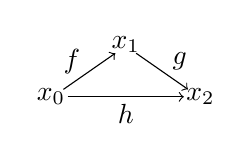
\begin{tikzpicture}[x=1.5em,y=1.5em]
  \node (x0) at (0,0) {$x_0$};
  \node (x1) at (1.8,1.25) {$x_1$};
  \node (x2) at (3.6,0) {$x_2$};
  \draw[->] (0.3,0.18) -- (1.55,1.05);
  \node at (0.5,0.85) {$f$};
  \draw[->] (2.05,1.05) -- (3.3,0.18);
  \node at (3.1,0.85) {$g$};
  \draw[->] (0.4,0) -- (3.2,0);
  \node at (1.8,-0.4) {$h$};
\end{tikzpicture}
\end{center}
这一关系特别地蕴含：\trHomotopy{}的 1-单纯形在\trHomotopyCategory{}中表示同一个箭头。
\end{definition}

1-\trCategory{}之\trNerve{}的\trHomotopyCategory\trIsomorphism{}于原来的\trCategory{}，因为\trNerve{}中的 2-\trSimplex{}见证了
底层\trReflexiveDirectedGraph{}的箭头所满足的全部合成关系。事实上，自然\trIsomorphism
$\mathrm{h}C\cong C$ 构成一个\trAdjunction{}的余单位（counit），
它把 $\mathcal{C}at$ 嵌入为 $s\mathcal{S}et$ 的反射子\trCategory
（reflective subcategory）。

\begin{proposition}\label{prop:nerve-left-adjoint}
\trNerve{}嵌入有左\trAdjunction{}，即把\trSimplicialSet{}送到其\trHomotopyCategory{}的\trFunctor{}：
\begin{center}
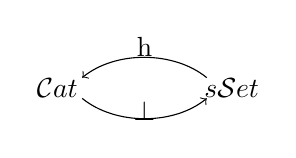
\begin{tikzpicture}[x=1.5em,y=1.5em]
  \node (cat) at (0,0) {$\mathcal{C}at$};
  \node (sset) at (4.2,0) {$s\mathcal{S}et$};
  \draw[->] (3.6,0.25) .. controls (2.8,0.9) and (1.4,0.9) .. (0.6,0.25);
  \node at (2.1,1.0) {$\mathrm{h}$};
  \draw[->] (0.6,-0.25) .. controls (1.4,-0.9) and (2.8,-0.9) .. (3.6,-0.25);
  \node at (2.1,-0.55) {$\perp$};
\end{tikzpicture}
\end{center}
\end{proposition}

\cref{prop:nerve-left-adjoint}的\trAdjunction{}对出于形式理由即可存在
（见\cref{ex:nerve-cosimplicial}），但直接的证明仍富有启发性。

\begin{proof}
对任何\trSimplicialSet $X$，都存在从 $X$ 到其\trHomotopyCategory{}之\trNerve $\mathrm{h}X$ 的自然
映射；由于\trNerve{}是\trTwoCoskeletal{}，只需定义 $\mathrm{sk}_2\,X\to\mathrm{h}X$，
而这由\cref{def:homotopy-category}的构造立即给出。注意：把\trHomotopyCategory\trFunctor
作用于商映射 $X\to\mathrm{h}X$ 后它变成\trIsomorphism{}，而且只要 $X$ 本是某个\trCategory{}的%
\trNerve{}，它就已经是\trIsomorphism{}。于是\trAdjunction{}性由引理 B.4.2 得出，%
也可直接验证三角形等式。
\end{proof}

\trQuasiCategory{}的\trHomotopyCategory{}容许一个简化了的描述。

\begin{lemma}[\trQuasiCategory{}的\trHomotopyCategory]\label{lem:homotopy-category-quasi-category}
若 $A$ 是\trQuasiCategory{}，则它的\textbf{\trHomotopyCategory} $\mathrm{h}A$ 具有：
\begin{itemize}
\item 对象：0-\trSimplex{}之集 $A_0$；
\item 箭头：1-\trSimplex{}之集 $A_1$ 的各\trHomotopy{}类；
\item 在 $a\in A_0$ 处的恒等箭头：由退化 1-\trSimplex{} $a\cdot\sigma^0\in A_1$
所表示；
\item $\mathrm{h}A$ 中的合成关系 $h=g\circ f$：对任意给定的 1-\trSimplex
$f$，$g$，$h\in A_1$ 所表示的箭头的\trHomotopy{}类而言，$h=g\circ f$ 成立当且仅当
存在一个边界为
\begin{center}
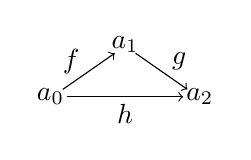
\begin{tikzpicture}[x=1.5em,y=1.5em]
  \node (a0) at (0,0) {$a_0$};
  \node (a1) at (1.8,1.25) {$a_1$};
  \node (a2) at (3.6,0) {$a_2$};
  \draw[->] (0.3,0.18) -- (1.55,1.05);
  \node at (0.5,0.85) {$f$};
  \draw[->] (2.05,1.05) -- (3.3,0.18);
  \node at (3.1,0.85) {$g$};
  \draw[->] (0.4,0) -- (3.2,0);
  \node at (1.8,-0.4) {$h$};
\end{tikzpicture}
\end{center}
的 2-\trSimplex{}。
\end{itemize}
\end{lemma}
\begin{proof}
见\cref{ex:homotopy-category-free-category}。
\end{proof}

\begin{definition}[\trQuasiCategory{}中的\trIsomorphism]\label{def:isomorphism-quasi-category}
\trQuasiCategory{}中的 1-\trSimplex{}是\textbf{\trIsomorphism}（isomorphism），\footnote{Joyal 称这些
映射为「\trIsomorphism」（isomorphism），而 Lurie 称之为「\trEquivalence」（equivalence）。
我们尽可能让\trInfinityCategory{}性概念与相应的 1-\trCategory{}性概念共用同一个称呼。}当且仅当
它在\trHomotopyCategory{}中表示一个\trIsomorphism{}。由\cref{lem:homotopy-category-quasi-category}，
这意味着：$f\colon a\to b$ 是\trIsomorphism{}，当且仅当存在 1-\trSimplex
$f^{-1}\colon b\to a$ 连同一对 2-\trSimplex
\begin{center}
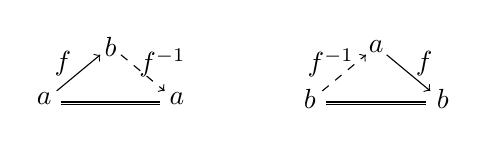
\begin{tikzpicture}[x=1.5em,y=1.5em]
  \node (a) at (0,0) {$a$};
  \node (b) at (1.6,1.25) {$b$};
  \node (a2) at (3.2,0) {$a$};
  \draw[->] (0.3,0.18) -- (1.35,1.05);
  \node at (0.45,0.85) {$f$};
  \draw[->,dashed] (1.85,1.05) -- (2.9,0.18);
  \node at (2.85,0.85) {$f^{-1}$};
  \draw[double] (0.4,-0.12) -- (2.8,-0.12);
  \node (b2) at (6.4,0) {$b$};
  \node (a3) at (8.0,1.25) {$a$};
  \node (b3) at (9.6,0) {$b$};
  \draw[->,dashed] (6.7,0.18) -- (7.75,1.05);
  \node at (6.9,0.85) {$f^{-1}$};
  \draw[->] (8.25,1.05) -- (9.3,0.18);
  \node at (9.15,0.85) {$f$};
  \draw[double] (6.8,-0.12) -- (9.2,-0.12);
\end{tikzpicture}
\end{center}
\end{definition}

\trQuasiCategory{}中\trIsomorphism{}的性质，最容易在一个密切相关的\trCategory{}中论证：那里的%
\trSimplicialSet{}带有额外的结构——在指定的 1-单纯形子集上做一个「标记」（marking）；
这些所谓的\textbf{\trMarkedSimplicialSet}（marked simplicial set）之间的
映射必须保持标记（见定义 D.1.1）。%
例如，每个\trQuasiCategory{}都有一个\emph{自然标记}（natural marking），其中带标记的
1-单纯形恰好是全部\trIsomorphism{}（见定义 D.4.5）。%
由于「\trQuasiCategory{}中是\trIsomorphism」这一性质由具有特定边界的 2-\trSimplex{}之存在所见证，
\trQuasiCategory{}之间的每个映射都保持\trIsomorphism{}，从而诱导出相应的自然带标记\trQuasiCategory{}之间的
映射。\trMarkedSimplicialSet{}很少出现在关于\trQuasiCategory{}中\trIsomorphism{}的某些组合引理的证明之外，
故细节留待附录 D。

现在来引出用标记技术证明的若干结果中的第一个。\trQuasiCategory $A$ 按定义沿一切
内\trHorn{}都有\trExtension{}。但当外\trHorn $\Lambda^0[2]\to A$ 或 $\Lambda^2[2]\to A$
的始边、终边（视情形而定）映成 $A$ 中的\trIsomorphism{}时，直觉上应当存在\trFiller

\begin{center}
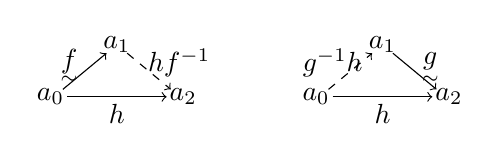
\begin{tikzpicture}[x=1.5em,y=1.5em]
  \node (a0) at (0,0) {$a_0$};
  \node (a1) at (1.6,1.25) {$a_1$};
  \node (a2) at (3.2,0) {$a_2$};
  \draw[->] (0.3,0.18) -- (1.35,1.05);
  \node at (0.45,0.85) {$f$};
  \node at (0.45,0.42) {$\scriptstyle\sim$};
  \draw[->,dashed] (1.85,1.05) -- (2.9,0.18);
  \node at (3.1,0.82) {$hf^{-1}$};
  \draw[->] (0.4,0) -- (2.8,0);
  \node at (1.6,-0.4) {$h$};
  \node (b0) at (6.4,0) {$a_0$};
  \node (b1) at (8.0,1.25) {$a_1$};
  \node (b2) at (9.6,0) {$a_2$};
  \draw[->,dashed] (6.7,0.18) -- (7.75,1.05);
  \node at (6.8,0.82) {$g^{-1}h$};
  \draw[->] (8.25,1.05) -- (9.3,0.18);
  \node at (9.15,0.85) {$g$};
  \node at (9.15,0.42) {$\scriptstyle\sim$};
  \draw[->] (6.8,0) -- (9.2,0);
  \node at (8.0,-0.4) {$h$};
\end{tikzpicture}
\end{center}
高维的「特殊外\trHorn」的表现类似：

\begin{proposition}[特殊外\trHorn{}填充]\label{prop:special-outer-horn-filling}
任何\trQuasiCategory $A$ 对下面这些外\trHorn
\begin{center}
\begin{tikzpicture}[x=1.4em,y=1.4em]
  \node (tl) at (0,1.2) {$\Lambda^0[n]$};
  \node (tr) at (3.0,1.2) {$A$};
  \node (bl) at (0,0) {$\Delta[n]$};
  \draw[->] (tl) -- (tr);
  \node at (1.5,1.52) {$g$};
  \draw[->] (0,0.85) -- (0,0.28);
  \draw (0,0.85) arc[start angle=180,end angle=0,radius=0.15];
  \draw[->,dashed] (0.5,0.22) -- (2.7,1.05);
  \node (tl2) at (6.6,1.2) {$\Lambda^n[n]$};
  \node (tr2) at (9.6,1.2) {$A$};
  \node (bl2) at (6.6,0) {$\Delta[n]$};
  \draw[->] (tl2) -- (tr2);
  \node at (8.1,1.52) {$h$};
  \draw[->] (6.6,0.85) -- (6.6,0.28);
  \draw (6.6,0.85) arc[start angle=180,end angle=0,radius=0.15];
  \draw[->,dashed] (7.1,0.22) -- (9.3,1.05);
  \node at (11.8,0.6) {对 $n\ge 1$};
\end{tikzpicture}
\end{center}
都有\trFiller{}，只要其中边 $g|_{\langle\,0,1\,\rangle}$ 与 $h|_{\langle\,n-1,n\,\rangle}$ 是\trIsomorphism{}。
\footnote{当 $n=1$ 时，对\trHorn{}无须任何条件；退化 1-\trSimplex{}给出所需的\trLifting{}。}
\end{proposition}

\cref{prop:special-outer-horn-filling}的证明需要归功于 Joyal 的巧妙组合
技术，我们将其推延到命题 D.4.6。%
这里且先坐享其众多推论。立即可得：

\begin{corollary}\label{cor:kan-groupoid}
\trQuasiCategory{}是\trKanComplex{}，当且仅当它的\trHomotopyCategory{}是\trGroupoid{}（groupoid）。
\end{corollary}
\begin{proof}
若\trQuasiCategory{}的\trHomotopyCategory{}是\trGroupoid{}，则它的全部 1-\trSimplex{}都是\trIsomorphism{}，于是
\cref{prop:special-outer-horn-filling}蕴含一切内、外\trHorn{}都有\trFiller{}，
因此该\trQuasiCategory{}是\trKanComplex{}。反之，在\trKanComplex{}中一切外\trHorn{}都可填充；
特别地，\cref{def:isomorphism-quasi-category}中所示的那些\trHorn{}的\trFiller
可用来为任何 1-\trSimplex{}构造左逆与右逆，再由
\cref{lem:homotopy-category-quasi-category}把它们矫正成单一的双侧逆。
\end{proof}

\trQuasiCategory $A$ 含有一个典范的\textbf{\trMaximalSubKanComplex}（maximal sub Kan
complex）$A^{\simeq}$，即由那些作为\trIsomorphism{}的 1-\trSimplex{}张成的单纯子集。
正如\trQuasiCategory $A$ 中的箭头由\trSimplicialSet{}映射 $\qcTwo\to A$ 表示——其定义域是
\emph{\trFreeLivingArrow}（free-living arrow）的\trNerve——\trQuasiCategory{}中的\trIsomorphism{}也可以由图形
$\qcInt\to A$ 表示，其定义域称作\textbf{\trHomotopyCoherentIsomorphism}（homotopy
coherent isomorphism），即\emph{\trFreeLivingIsomorphism}（free-living isomorphism）的\trNerve{}：

\begin{corollary}\label{cor:hc-isomorphism}
\trQuasiCategory $A$ 中的箭头 $f$ 是\trIsomorphism{}，当且仅当它可\trExtension{}成一个\trHomotopyCoherentIsomorphism
\begin{center}
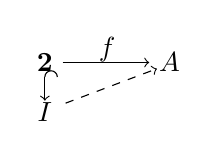
\begin{tikzpicture}[x=1.5em,y=1.5em]
  \node (tl) at (0,1.2) {$\qcTwo$};
  \node (tr) at (3.0,1.2) {$A$};
  \node (bl) at (0,0) {$\qcInt$};
  \draw[->] (tl) -- (tr);
  \node at (1.5,1.52) {$f$};
  \draw[->] (0,0.85) -- (0,0.28);
  \draw (0,0.85) arc[start angle=180,end angle=0,radius=0.15];
  \draw[->,dashed] (0.5,0.22) -- (2.7,1.05);
\end{tikzpicture}
\end{center}
\end{corollary}
\begin{proof}
若 $f$ 是\trIsomorphism{}，则映射 $f\colon\qcTwo\to A$ 落入含于 $A$ 中的极大子%
\trKanComplex{}：
\begin{center}
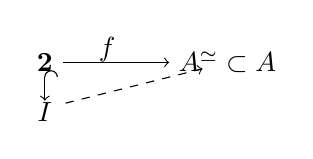
\begin{tikzpicture}[x=1.5em,y=1.5em]
  \node (tl) at (0,1.2) {$\qcTwo$};
  \node (tr) at (4.4,1.2) {$A^{\simeq}\subset A$};
  \node (bl) at (0,0) {$\qcInt$};
  \draw[->] (tl) -- (tr);
  \node at (1.5,1.52) {$f$};
  \draw[->] (0,0.85) -- (0,0.28);
  \draw (0,0.85) arc[start angle=180,end angle=0,radius=0.15];
  \draw[->,dashed] (0.5,0.22) -- (3.8,1.05);
\end{tikzpicture}
\end{center}
由\cref{ex:free-living-isomorphism}，包含 $\qcTwo\hookrightarrow\qcInt$
可以表示成外\trHorn{}包含之\trPushout{}（pushout）的序列复合。由于 $A^{\simeq}$ 是%
\trKanComplex{}，这表明所需的\trExtension{}存在，而且实际上落入 $A^{\simeq}\subset A$。
\end{proof}

\trSimplicialSet{}的\trCategory{}如同任何预层\trCategory{}一样是\trCartesianClosed{}。
由\trYonedaLemma{}与定义性\trAdjunction{}，指数 $Y^X$ 中的 $n$-\trSimplex{}对应于%
\trSimplicialSet{}映射 $X\times\Delta[n]\to Y$，它的面与退化通过在\trSimplex{}变量中预合成
来计算。我们的下一个目标是证明：\trQuasiCategory{}构成\trSimplicialSet{}这个\trSimpliciallyEnrichedCategory{}中的一个
\textbf{\trExponentialIdeal}（exponential ideal）：若 $X$ 是\trSimplicialSet{}而 $A$ 是\trQuasiCategory{}，
则 $A^X$ 是\trQuasiCategory{}。我们将把它当作该结果之「相对」版本的推论导出，后者涉及
一类叫做\trIsofibration{}的映射，现在就来引入。

\begin{definition}[\trIsofibration]\label{def:isofibration}
\trQuasiCategory{}之间的\trSimplicialSet{}映射 $f\colon A\to B$ 是一个\textbf{\trIsofibration}
（isofibration），若它对内\trHorn{}包含——如左下图所示——以及任一顶点向自由%
\trIsomorphism $\qcInt$ 的包含都能\trLifting{}：
\begin{center}
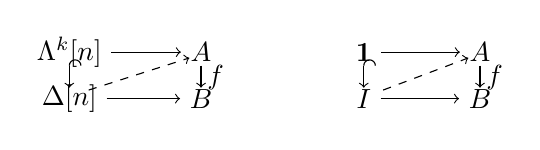
\begin{tikzpicture}[x=1.4em,y=1.4em]
  \node (tl) at (0,1.2) {$\Lambda^k[n]$};
  \node (tr) at (3.4,1.2) {$A$};
  \node (bl) at (0,0) {$\Delta[n]$};
  \node (br) at (3.4,0) {$B$};
  \draw[->] (tl) -- (tr);
  \draw[->] (0,0.85) -- (0,0.28);
  \draw (0,0.85) arc[start angle=180,end angle=0,radius=0.15];
  \draw[->,dashed] (0.5,0.22) -- (3.1,1.05);
  \draw[->] (3.4,0.85) -- (3.4,0.28);
  \node at (3.78,0.55) {$f$};
  \draw[->] (bl) -- (br);
  \node (tl2) at (7.6,1.2) {$\qcOne$};
  \node (tr2) at (10.6,1.2) {$A$};
  \node (bl2) at (7.6,0) {$\qcInt$};
  \node (br2) at (10.6,0) {$B$};
  \draw[->] (tl2) -- (tr2);
  \draw[->] (7.6,0.85) -- (7.6,0.28);
  \draw (7.6,0.85) arc[start angle=180,end angle=0,radius=0.15];
  \draw[->,dashed] (8.1,0.22) -- (10.3,1.05);
  \draw[->] (10.6,0.85) -- (10.6,0.28);
  \node at (10.98,0.55) {$f$};
  \draw[->] (bl2) -- (br2);
\end{tikzpicture}
\end{center}
为了在记号上区分\trIsofibration{}，我们把它们画成带两个头的箭头
「$\twoheadrightarrow$」。
\end{definition}

命题 1.1.14 被其相对化类比所吸收，后者证为定理 D.5.1：%

\begin{proposition}[特殊外\trHorn\trLifting]\label{prop:special-outer-horn-lifting}
\trQuasiCategory{}之间的任何\trIsofibration $f\colon A\twoheadrightarrow B$ 对下面这些
外\trHorn
\begin{center}
\begin{tikzpicture}[x=1.4em,y=1.4em]
  \node (tl) at (0,1.2) {$\Lambda^0[n]$};
  \node (tr) at (3.4,1.2) {$A$};
  \node (bl) at (0,0) {$\Delta[n]$};
  \node (br) at (3.4,0) {$B$};
  \draw[->] (tl) -- (tr);
  \node at (1.5,1.52) {$g$};
  \draw[->] (0,0.85) -- (0,0.28);
  \draw (0,0.85) arc[start angle=180,end angle=0,radius=0.15];
  \draw[->,dashed] (0.5,0.22) -- (3.1,1.05);
  \draw[->] (3.4,0.85) -- (3.4,0.28);
  \node at (3.78,0.55) {$f$};
  \draw[->] (bl) -- (br);
  \node at (1.7,-0.38) {$k$};
  \node (tl2) at (7.6,1.2) {$\Lambda^n[n]$};
  \node (tr2) at (11.0,1.2) {$A$};
  \node (bl2) at (7.6,0) {$\Delta[n]$};
  \node (br2) at (11.0,0) {$B$};
  \draw[->] (tl2) -- (tr2);
  \node at (9.3,1.52) {$h$};
  \draw[->] (7.6,0.85) -- (7.6,0.28);
  \draw (7.6,0.85) arc[start angle=180,end angle=0,radius=0.15];
  \draw[->,dashed] (8.1,0.22) -- (10.7,1.05);
  \draw[->] (11.0,0.85) -- (11.0,0.28);
  \node at (11.38,0.55) {$f$};
  \draw[->] (bl2) -- (br2);
  \node at (9.3,-0.38) {$\ell$};
  \node at (13.4,0.6) {对 $n\ge 1$};
\end{tikzpicture}
\end{center}
都有\trLifting{}，只要其中边 $g|_{\langle\,0,1\,\rangle}$、$h|_{\langle\,n-1,n\,\rangle}$、$k|_{\langle\,0,1\,\rangle}$ 与
$\ell|_{\langle\,n-1,n\,\rangle}$ 都是\trIsomorphism{}。
\end{proposition}

\begin{observation}\label{obs:isofibration-basics}
\begin{enumerate}[label=(\roman*)]
\item 对任何\trSimplicialSet $X$，以\trTerminal{}\trSimplicialSet 1 为陪域的唯一映射 $X\to 1$
是\trIsofibration{}，当且仅当 $X$ 是\trQuasiCategory{}。
\item 任何由右提升性质（right lifting property）刻画的映射类——例如\trIsofibration{}——
都自动对合成、乘积、\trPullback{}（pullback）、收缩（retract）以及塔的
（逆）\trLimit{}封闭（见引理 C.2.3）。%
\item 把 (i) 与 (ii) 结合起来：若 $A\twoheadrightarrow B$ 是\trIsofibration{}，而 $B$ 是%
\trQuasiCategory{}，则 $A$ 也是。
\item \trIsofibration{}推广了那个同名的范畴论概念。\trCategory{}之间任何%
\trFunctor{} $f\colon A\to B$ 的\trNerve{}定义了一个对内\trHorn{}包含可\trLifting{}的\trSimplicialSet
映射。这个映射定义\trIsofibration{}，当且仅当：对 $B$ 中的任何\trIsomorphism{}以及 $A$ 中%
\trLifting{}其定义域或陪域的指定对象，$A$ 中总存在具有该定义域或陪域、且\trLifting{}该%
\trIsomorphism{}的\trIsomorphism{}。
\end{enumerate}
\end{observation}

难以建立得多的是\trIsofibration{}在「Leibniz\footnote{这个名字暗指微分学中的
Leibniz 法则，更确切地，暗指把引理 D.3.1 的\trLeibnizProduct{}的定义域等同于
棱柱（prism）的边界（见定义 C.2.8 与注 D.3.2）。}%
指数」（Leibniz exponential）构造下的稳定性，如图
\eqref{eq:leibniz-exponential}所示。这将由命题 D.5.2 证明。

\begin{proposition}\label{prop:leibniz-exponential}
若 $i\colon X\hookrightarrow Y$ 是\trMonomorphism{}，而
$f\colon A\twoheadrightarrow B$ 是\trIsofibration{}，那么诱导的 Leibniz 指数
映射 $i\widehat{\pitchfork}f$
\begin{rveq}\label{eq:leibniz-exponential}
\mbox{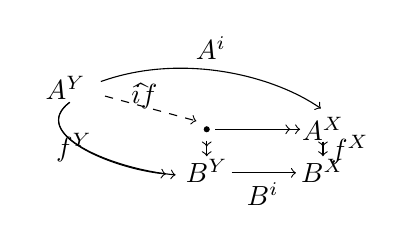
\begin{tikzpicture}[x=1.5em,y=1.5em]
  \node (AY) at (0,2.0) {$A^Y$};
  \fill (3.4,1.0) circle (1.1pt);
  \node (AX) at (6.2,1.0) {$A^X$};
  \node (BY) at (3.4,0) {$B^Y$};
  \node (BX) at (6.2,0) {$B^X$};
  \draw[->] (0.85,2.15) .. controls (2.8,2.85) and (5.0,2.3) .. (6.15,1.5);
  \node at (3.5,2.95) {$A^i$};
  \draw[->] (0.1,1.65) .. controls (-0.9,0.9) and (1.1,0.05) .. (2.65,-0.1);
  \draw[->,shorten >=0.35em] (0.1,1.65) .. controls (-0.9,0.9) and (1.1,0.05) .. (2.65,-0.1);
  \node at (0.2,0.55) {$f^Y$};
  \draw[->,dashed] (0.95,1.8) -- (3.15,1.2);
  \node at (1.9,1.8) {$i\widehat{\pitchfork}f$};
  \draw[->] (3.6,1.0) -- (5.65,1.0);
  \draw[->,shorten >=0.35em] (3.6,1.0) -- (5.65,1.0);
  \draw[->] (3.4,0.72) -- (3.4,0.35);
  \draw[->,shorten >=0.35em] (3.4,0.72) -- (3.4,0.35);
  \draw[->] (6.2,0.7) -- (6.2,0.35);
  \draw[->,shorten >=0.35em] (6.2,0.7) -- (6.2,0.35);
  \node at (6.85,0.5) {$f^X$};
  \draw[->] (4.0,-0.05) -- (5.55,-0.05);
  \node at (4.75,-0.55) {$B^i$};
  \node at (3.85,0.6) {$\lrcorner$};
\end{tikzpicture}}
\end{rveq}
仍是\trIsofibration{}。\footnote{这一结果的退化情形——取 $X=\varnothing$ 或
$B=1$——蕴含图中其余六个映射也都是\trIsofibration
（见\cref{ex:leibniz-specialization}）。}
\end{proposition}

\begin{corollary}\label{cor:exponential-ideal}
若 $X$ 是\trSimplicialSet{}而 $A$ 是\trQuasiCategory{}，则 $A^X$ 是\trQuasiCategory{}。此外，$A^X$ 中的
1-\trSimplex{}是\trIsomorphism{}，当且仅当它在 $X$ 的每个顶点处的分量都是 $A$ 中的\trIsomorphism{}。
\end{corollary}
\begin{proof}
第一句话是\cref{prop:leibniz-exponential}的特例
（见\cref{ex:leibniz-specialization}）；第二句话的证明类似，用带标记%
\trSimplicialSet{}来论证（见推论 D.4.19）。%
\end{proof}

\begin{definition}[\trQuasiCategory{}间的\trEquivalence]\label{def:equivalences-quasi-categories}
\trQuasiCategory{}之间的映射 $f\colon A\to B$ 是一个\textbf{\trEquivalence}
（equivalence），若它能\trExtension{}成一份以\trFreeLivingIsomorphism $\qcInt$ 充当区间
（interval）的「\trHomotopy\trEquivalence」数据；也就是说，若存在映射 $g\colon B\to A$，
\begin{center}
\begin{tikzpicture}[x=1.5em,y=1.5em]
  \node (Al) at (0,1.0) {$A$};
  \node (Ac) at (2.4,1.0) {$A^{\qcInt}$};
  \node (At) at (4.6,2.4) {$A$};
  \node (Ab) at (4.6,-0.4) {$A$};
  \draw[->] (0.4,1.0) -- (1.6,1.0);
  \node at (1.0,1.3) {$\alpha$};
  \draw[->] (2.7,1.3) -- (4.25,2.2);
  \node at (3.85,2.0) {$\mathrm{ev}_0$};
  \draw[->] (2.7,0.7) -- (4.25,-0.2);
  \node at (3.85,-0.1) {$\mathrm{ev}_1$};
  \draw[double] (0.35,1.4) -- (4.1,2.45);
  \draw[->] (0.4,0.6) -- (4.2,-0.28);
  \node at (1.7,0.02) {$gf$};
  \node at (7.4,1.0) {及};
  \node (Bl) at (10.0,1.0) {$B$};
  \node (Bc) at (12.4,1.0) {$B^{\qcInt}$};
  \node (Bt) at (14.6,2.4) {$B$};
  \node (Bb) at (14.6,-0.4) {$B$};
  \draw[->] (10.35,1.35) -- (14.1,2.45);
  \node at (11.3,2.15) {$fg$};
  \draw[->] (10.4,1.0) -- (11.6,1.0);
  \node at (11.0,1.3) {$\beta$};
  \draw[->] (12.7,1.3) -- (14.25,2.2);
  \node at (13.85,2.0) {$\mathrm{ev}_0$};
  \draw[->] (12.7,0.7) -- (14.25,-0.2);
  \node at (13.85,-0.1) {$\mathrm{ev}_1$};
  \draw[double] (10.35,0.6) -- (14.1,-0.35);
\end{tikzpicture}
\end{center}
我们写「$\qcEquiv$」来装饰\trEquivalence{}，并以 $A\simeq B$ 表示存在\trEquivalence
$A\qcEquiv B$。
\end{definition}

\begin{remark}\label{rem:hf-equivalence}
若 $f\colon A\to B$ 是\trQuasiCategory{}之间的\trEquivalence{}，则\trFunctor
$\mathrm{h}f\colon\mathrm{h}A\to\mathrm{h}B$ 是\trCategory{}的\trEquivalence{}；上面展示的
数据定义了\trEquivalence{}逆 $\mathrm{h}g\colon\mathrm{h}B\to\mathrm{h}A$ 以及由
复合\trFunctor\footnote{注意 $\mathrm{h}(A^{\qcInt})$ 与
$(\mathrm{h}A)^{\qcInt}$ 一般并不\trIsomorphism{}。后者中的对象是 $A$ 中\trIsomorphism{}的%
\trHomotopy{}类；前者中的对象则是\trHomotopyCoherentIsomorphism——由 $A$ 中一个指定的 1-单纯形、
一个指定的逆 1-单纯形，连同由 $\qcInt$ 的非退化单纯形标引的
相干性数据的无穷之塔给出。}编码而成的自然\trIsomorphism{}：
\[
\mathrm{h}A\xrightarrow{\;\mathrm{h}\alpha\;}\mathrm{h}(A^{\qcInt})
\longrightarrow(\mathrm{h}A)^{\qcInt}
\qquad\qquad
\mathrm{h}B\xrightarrow{\;\mathrm{h}\beta\;}\mathrm{h}(B^{\qcInt})
\longrightarrow(\mathrm{h}B)^{\qcInt}
\]
\end{remark}

\begin{definition}\label{def:trivial-fibration}
\trSimplicialSet{}之间的映射 $f\colon X\to Y$ 是一个\textbf{\trTrivialFibration}
（trivial fibration），若它对一切单纯形的边界包含都能\trLifting{}：
\begin{rveq}\label{eq:trivial-fibration}
\mbox{\begin{tikzpicture}[x=1.5em,y=1.5em]
  \node (tl) at (0,1.2) {$\partial\Delta[n]$};
  \node (tr) at (3.4,1.2) {$X$};
  \node (bl) at (0,0) {$\Delta[n]$};
  \node (br) at (3.4,0) {$Y$};
  \draw[->] (tl) -- (tr);
  \draw[->] (0,0.85) -- (0,0.28);
  \draw (0,0.85) arc[start angle=180,end angle=0,radius=0.15];
  \draw[->,dashed] (0.5,0.22) -- (3.1,1.05);
  \draw[->] (3.4,0.85) -- (3.4,0.28);
  \draw[->,shorten >=0.35em] (3.4,0.85) -- (3.4,0.28);
  \node at (3.0,0.55) {$\wr$};
  \node at (3.82,0.55) {$f$};
  \draw[->] (bl) -- (br);
  \node at (8.0,0.6) {对 $n\ge 0$};
\end{tikzpicture}}
\end{rveq}
我们写「$\qcTFib$」来装饰\trTrivialFibration{}。
\end{definition}

\begin{remark}\label{rem:trivial-fibration-notation}
\trSimplex{}边界包含 $\partial\Delta[n]\hookrightarrow\Delta[n]$
「\trCell{}式地生成」（cellularly generate）\trSimplicialSet{}的\trMonomorphism
（见定义 C.2.4 与引理 C.5.9）。%
于是引理 C.2.3 的对偶命题蕴含：\trTrivialFibration{}对\trSimplicialSet{}之间的任何\trMonomorphism{}都能%
\trLifting{}。特别地，由此可知任何\trTrivialFibration $X\qcTFib Y$ 都是\trSplitEpimorphism
（split epimorphism）。

记号「$\qcTFib$」是有暗示意味的：\trQuasiCategory{}之间的\trTrivialFibration{}恰好就是那些既是%
\trIsofibration{}又是\trEquivalence{}的映射。这一点可以用单纯\trHomotopy{}论中一个相当标准、只是
颇为技术性的论证来证明，见命题 D.5.6。%
\end{remark}

\begin{proposition}\label{prop:trivial-fibration-characterization}
对\trQuasiCategory{}之间的映射 $f\colon A\to B$，下列诸条件\trEquivalence{}：
\begin{enumerate}[label=(\roman*)]
\item $f$ 是\trTrivialFibration{}；
\item $f$ 既是\trIsofibration{}又是\trEquivalence{}；
\item $f$ 是\textbf{\trSplitFiberHomotopyEquivalence}（split fiber homotopy
equivalence）：一个\trIsofibration{}，它容许一个\trSection{}（section）$s$，这个截面
经由从 $\mathrm{id}_A$ 到 $sf$ 的\trHomotopy $\alpha$ 而成为\trEquivalence{}逆，且该\trHomotopy{}与
$f$ 复合后给出从 $f$ 到 $f$ 的常值\trHomotopy{}。
\begin{center}
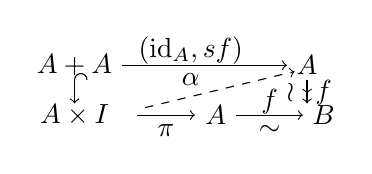
\begin{tikzpicture}[x=1.5em,y=1.5em]
  \node (tl) at (0,1.2) {$A+A$};
  \node (tr) at (5.6,1.2) {$A$};
  \node (bl) at (0,0) {$A\times\qcInt$};
  \node (bm) at (3.4,0) {$A$};
  \node (br) at (6.0,0) {$B$};
  \draw[->] (tl) -- (tr);
  \node at (2.8,1.55) {$(\mathrm{id}_A,sf)$};
  \draw[->] (0,0.85) -- (0,0.28);
  \draw (0,0.85) arc[start angle=180,end angle=0,radius=0.15];
  \draw[->,dashed] (1.7,0.18) -- (5.3,1.05);
  \node at (2.8,0.85) {$\alpha$};
  \draw[->] (5.6,0.85) -- (5.6,0.28);
  \draw[->,shorten >=0.35em] (5.6,0.85) -- (5.6,0.28);
  \node at (5.2,0.55) {$\wr$};
  \node at (6.0,0.55) {$f$};
  \draw[->] (1.5,0) -- (2.9,0);
  \node at (2.2,-0.38) {$\pi$};
  \draw[->] (3.9,0) -- (5.5,0);
  \node at (4.7,0.32) {$f$};
  \node at (4.7,-0.38) {$\sim$};
\end{tikzpicture}
\end{center}
\end{enumerate}
\end{proposition}

作为由右提升性质刻画的类，\trTrivialFibration{}还对合成、乘积、\trPullback{}与塔的%
\trLimit{}封闭，并且包含全部\trIsomorphism{}。这些映射在 Leibniz 指数化下的稳定性，
与\cref{prop:leibniz-exponential}一起在命题 D.5.2 中得到证明。

\begin{proposition}\label{prop:leibniz-exponential-trivial}
若 $i\colon X\hookrightarrow Y$ 是\trMonomorphism{}而 $f\colon A\twoheadrightarrow B$
是\trIsofibration{}，那么当 $f$ 是\trTrivialFibration{}，或者 $i$ 属于由内\trHorn{}包含与映射
$\qcOne\hookrightarrow\qcInt$ \trCell{}式生成的类时，诱导的 Leibniz 指数映射
\[
A^Y\xrightarrow{\;i\widehat{\pitchfork}f\;}B^Y\times_{B^X}A^X
\]
是\trTrivialFibration{}。
\end{proposition}

为展示这些 Leibniz 稳定性结果的效用，我们给出\trKanComplex{}的一个「内蕴的」
或「综合的」刻画。

\begin{lemma}\label{lem:kan-internal}
\trQuasiCategory $A$ 是\trKanComplex{}，当且仅当由包含 $\qcTwo\hookrightarrow\qcInt$
诱导的映射 $A^{\qcInt}\qcTFib A^{\qcTwo}$ 是\trTrivialFibration{}。
\end{lemma}

注意\cref{prop:leibniz-exponential}蕴含
$A^{\qcInt}\twoheadrightarrow A^{\qcTwo}$ 是\trIsofibration{}。
\begin{proof}
刻画\trTrivialFibration{}的那个提升性质可以转置成另一个提升性质，如右下图所示：
\begin{center}
\begin{tikzpicture}[x=1.4em,y=1.4em]
  \node (tl) at (0,1.2) {$\partial\Delta[n]$};
  \node (tr) at (3.4,1.2) {$A^{\qcInt}$};
  \node (bl) at (0,0) {$\Delta[n]$};
  \node (br) at (3.4,0) {$A^{\qcTwo}$};
  \draw[->] (tl) -- (tr);
  \draw[->] (0,0.85) -- (0,0.28);
  \draw (0,0.85) arc[start angle=180,end angle=0,radius=0.15];
  \draw[->,dashed] (0.5,0.22) -- (3.1,1.05);
  \draw[->] (3.4,0.85) -- (3.4,0.28);
  \draw[->] (bl) -- (br);
  \node at (6.6,0.6) {$\leftrightsquigarrow$};
  \node (TL) at (11.2,1.2)
    {$\partial\Delta[n]\times\qcInt\;\underset{\partial\Delta[n]\times\qcTwo}{\cup}\;\Delta[n]\times\qcTwo$};
  \node (TR) at (18.6,1.2) {$A$};
  \node (BL) at (11.2,0) {$\Delta[n]\times\qcInt$};
  \draw[->] (TL) -- (TR);
  \draw[->] (11.2,0.85) -- (11.2,0.28);
  \draw (11.2,0.85) arc[start angle=180,end angle=0,radius=0.15];
  \draw[->,dashed] (11.8,0.15) -- (18.3,1.05);
\end{tikzpicture}
\end{center}
它断言：$A$ 沿这样一些映射有\trExtension——它们由\trSimplex{}边界包含
$\partial\Delta[n]\hookrightarrow\Delta[n]$ 与包含
$\qcTwo\hookrightarrow\qcInt$ 作 \emph{\trLeibnizProduct}（Leibniz product，
又称\trPushout{}积（pushout product））而得。由\cref{ex:free-living-isomorphism}(ii)，
包含 $\qcTwo\hookrightarrow\qcInt$ 是左外\trHorn{}包含的\trPushout{}的序列复合。
由推论 D.3.11——它是通往\cref{prop:leibniz-exponential}与
\cref{prop:leibniz-exponential-trivial}之证明途中的关键一步——\trLeibnizProduct%
也是左外\trHorn{}包含与内\trHorn{}包含的\trPushout{}的序列复合。
若 $A$ 是\trKanComplex{}，则右上图所示的\trExtension{}存在，经转置便知
$A^{\qcInt}\qcTFib A^{\qcTwo}$ 是\trTrivialFibration{}。

反之，若 $A^{\qcInt}\qcTFib A^{\qcTwo}$ 是\trTrivialFibration{}，那么它特别地在
顶点上是满射。于是 $A$ 中的每个箭头都是\trIsomorphism{}，而\cref{cor:kan-groupoid}
告诉我们：$A$ 必定是\trKanComplex{}。
\end{proof}

\begin{digression}[Joyal \trModelStructure]\label{dig:joyal-model-structure}
\trSimplicialSet{}的\trCategory{}带有一个 Quillen 意义下（见定义 C.3.1）的
\textbf{\trModelStructure}（model structure），%
其\trFibrant{}对象（fibrant object）恰好是\trQuasiCategory{}，而且其中所有对象都是%
\trCofibrant{}的（cofibrant）。在\trFibrant{}对象之间，\trFibration{}、\trWeakEquivalence
（weak equivalence）与\trTrivialFibration{}恰是刚才引入的\trIsofibration{}、\trEquivalence{}与平凡%
\trFibration{}。\cref{prop:trivial-fibration-characterization}证明了\trTrivialFibration
是\trFibration{}与\trWeakEquivalence{}的交。\cref{prop:leibniz-exponential}与
\cref{prop:leibniz-exponential-trivial}则反映出：Joyal \trModelStructure{}是一个%
\trCartesianClosed\trModelCategory{}（cartesian closed model category），满足定义 C.3.10
的额外公理。%

我们不愿再进一步展开\trQuasiCategory{}上的 Joyal \trModelStructure{}，因为所需的全部特征都已
在此得到突出。这里列举的结果足以表明：\trQuasiCategory{}的\trCategory{}定义了一个%
\trInfinityCosmos——一个我们现在就要转入的概念。
\end{digression}

\subsection*{练习}

\begin{exercise}[\cite{bib103}~\S1.5]\label{ex:nerve-cosimplicial}
给定任意取值于任意\trCategory{} $\mathcal{E}$ 的\trCosimplicialObject
（cosimplicial object）$C\colon\Delta\to\mathcal{E}$，都有一个相伴的
\textbf{\trNerve{}函子} $N_C$，定义如下：
\[
\begin{array}{c}
\mathcal{E}\xrightarrow{\quad N_C\quad}s\mathcal{S}et\\[4pt]
E\longmapsto\mathrm{hom}(C^{-},E)
\end{array}
\qquad\qquad
\mbox{\begin{tikzpicture}[x=1.5em,y=1.5em]
  \node (D) at (2.4,2.1) {$\Delta$};
  \node (E) at (0,0) {$\mathcal{E}$};
  \node (S) at (4.8,0) {$s\mathcal{S}et$};
  \draw[->] (0.5,0.45) -- (1.95,1.8);
  \node at (0.65,1.35) {$C$};
  \draw[->] (2.85,1.8) -- (4.3,0.45);
  \node at (4.15,1.35) {よ};
  \draw[->] (4.25,0.2) .. controls (3.4,0.85) and (1.4,0.85) .. (0.55,0.2);
  \node at (2.4,0.98) {$\mathrm{lan}_{\text{よ}}C$};
  \node at (2.4,0.4) {$\perp$};
  \draw[->] (0.55,-0.2) .. controls (1.4,-0.75) and (3.4,-0.75) .. (4.25,-0.2);
  \node at (2.4,-1.05) {$N_C$};
\end{tikzpicture}}
\]
由构造，$N_CE$ 中的 $n$-\trSimplex{}对应 $\mathcal{E}$ 中的映射 $C^n\to E$。
证明：若 $\mathcal{E}$ \trCocomplete{}（cocomplete），则 $N_C$ 有左\trAdjunction{}，定义为%
\trFunctor{} $C$ 沿 \trYonedaEmbedding $\text{よ}\colon\Delta\hookrightarrow s\mathcal{S}et$ 的左\trKanExtension{}。这给出
\cref{prop:nerve-left-adjoint}的第二个证明。
\end{exercise}

\begin{exercise}[Boardman--Vogt；\cite{bib21}]\label{ex:homotopy-equivalence}
考虑\trQuasiCategory{}中以 $a$ 为\trInitial{}顶点、$b$ 为\trTerminal{}顶点的那些
1-单纯形之集。
\begin{enumerate}[label=(\roman*)]
\item 证明：由「$f\sim g$，当且仅当存在一个边界为
\tikz[baseline=-0.8ex]{\begin{scope}[x=1.3em,y=1.3em]
  \node (a) at (0,0) {$a$};
  \node (b) at (1.5,1.15) {$b$};
  \node (b2) at (3.0,0) {$b$};
  \draw[->] (0.28,0.16) -- (1.26,0.98);
  \node at (0.4,0.8) {$f$};
  \draw[double] (1.72,0.95) -- (2.72,0.14);
  \draw[->] (0.38,0) -- (2.62,0);
  \node at (1.5,-0.4) {$g$};
\end{scope}}
的 2-\trSimplex{}」所定义的关系是\trEquivalence{}关系。
\item 证明：由「$f\sim g$，当且仅当存在一个边界为
\tikz[baseline=-0.8ex]{\begin{scope}[x=1.3em,y=1.3em]
  \node (a) at (0,0) {$a$};
  \node (a2) at (1.5,1.15) {$a$};
  \node (b) at (3.0,0) {$b$};
  \draw[double] (0.28,0.14) -- (1.26,0.98);
  \draw[->] (1.74,0.98) -- (2.72,0.16);
  \node at (2.62,0.8) {$f$};
  \draw[->] (0.38,0) -- (2.62,0);
  \node at (1.5,-0.4) {$g$};
\end{scope}}
的 2-\trSimplex{}」所定义的关系是\trEquivalence{}关系。
\item 证明：(i) 与 (ii) 所定义的\trEquivalence{}关系是同一个。
\end{enumerate}
这就证明了\cref{lem:homotopic-quasi-category}。
\end{exercise}

\begin{exercise}\label{ex:homotopy-category-free-category}
考虑如下\trReflexiveDirectedGraph——它是一个\trQuasiCategory $A$ 的底层——上的\trFreeCategory{}：
\[
A_1\!
\begin{array}{@{}c@{}}
\xrightarrow{\;\cdot\delta^1\;}\\[-3pt]
\xleftarrow[\;\cdot\sigma^0\;]{}\\[-3pt]
\xrightarrow[\;\cdot\delta^0\;]{}
\end{array}
\!A_0,
\]
\begin{enumerate}[label=(\roman*)]
\item 考虑这样的二元关系：只要在 $A$ 的某个\trSimplex{}中，两列具有公共来源与
公共目标的可合成 1-\trSimplex{}给出从其\trInitial{}顶点到\trTerminal{}顶点的
两条路径，就把这两列等同起来。证明：这一关系对用 1-\trSimplex{}作合成前与
合成后是\trStable{}，并据此得出：它的\trTransitiveClosure{}是一个\textbf{\trCongruence}
（congruence）——即对合成前与合成后封闭的\trEquivalence{}关系。
\footnote{给定 1-\trCategory{}诸同态集上的一个\trCongruence{}关系，可以逐个同态集取商而
形成商范畴（见\cite{bib81}~\S II.8）。}
\item 考虑由强加合成关系 $h=g\circ f$ 所生成的\trCongruence{}关系——该关系由边界为
\tikz[baseline=-0.8ex]{\begin{scope}[x=1.3em,y=1.3em]
  \node (a0) at (0,0) {$a_0$};
  \node (a1) at (1.5,1.15) {$a_1$};
  \node (a2) at (3.0,0) {$a_2$};
  \draw[->] (0.28,0.16) -- (1.26,0.98);
  \node at (0.4,0.8) {$f$};
  \draw[->] (1.74,0.98) -- (2.72,0.16);
  \node at (2.62,0.8) {$g$};
  \draw[->] (0.38,0) -- (2.62,0);
  \node at (1.5,-0.4) {$h$};
\end{scope}}
的 2-\trSimplex{}见证——并证明它与 (i) 中所考虑的关系重合。
\item 在 (i) 与 (ii) 的\trCongruence{}关系中，证明：$A$ 中任何可合成 1-\trSimplex{}序列都\trEquivalence{}于单个
1-\trSimplex{}。据此得出：该\trFreeCategory{}对这个\trCongruence{}关系所取的商中的每个态射，都由
$A$ 中的一个 1-单纯形表示。
\item 证明：对 $A$ 中任意三个 1-\trSimplex{} $f$，$g$，$h$，在
\cref{def:homotopy-category}的\trHomotopyCategory $\mathrm{h}A$ 中 $h=g\circ f$
成立，当且仅当存在边界为
\tikz[baseline=-0.8ex]{\begin{scope}[x=1.3em,y=1.3em]
  \node (a0) at (0,0) {$a_0$};
  \node (a1) at (1.5,1.15) {$a_1$};
  \node (a2) at (3.0,0) {$a_2$};
  \draw[->] (0.28,0.16) -- (1.26,0.98);
  \node at (0.4,0.8) {$f$};
  \draw[->] (1.74,0.98) -- (2.72,0.16);
  \node at (2.62,0.8) {$g$};
  \draw[->] (0.38,0) -- (2.62,0);
  \node at (1.5,-0.4) {$h$};
\end{scope}}
的 2-\trSimplex{}。
\end{enumerate}
这就证明了\cref{lem:homotopy-category-quasi-category}。
\end{exercise}

\begin{exercise}\label{ex:unique-fillers}
证明：任何内\trHorn{}都有唯一\trFiller{}的\trQuasiCategory{}，\trIsomorphism{}于其\trHomotopyCategory{}的\trNerve{}。
\end{exercise}

\begin{exercise}\label{ex:free-living-isomorphism}
设 $\qcInt$ 是\trFreeLivingIsomorphism{}的\trNerve{}。
\begin{enumerate}[label=(\roman*)]
\item 证明：$\qcInt$ 在每个维数都恰有两个非退化\trSimplex{}。
\item 归纳地从 $\qcTwo$ 构筑出 $\qcInt$：把包含
$\qcTwo\hookrightarrow\qcInt$ 表示成左外\trHorn{}包含\footnote{按定义 1.2.25
所描述的对偶性，也可以换用右外\trHorn{}包含 $\Lambda^n[n]\hookrightarrow\Delta[n]$。}
$\Lambda^0[n]\hookrightarrow\Delta[n]$ 的\trPushout{}的序列复合，从 $n=2$ 开始
每维一个。\footnote{$\qcTwo\hookrightarrow\qcInt$ 的这一分解揭示了哪些
数据能\trHomotopy{}唯一地\trExtension{}成一个\trHomotopyCoherentIsomorphism{}。例如，\cref{def:isomorphism-quasi-category}
中的那些 1-\trSimplex{}与 2-\trSimplex{}，连同以它们为外表面而内表面皆退化的单个
3-\trSimplex{}。\trHomotopy{}类型论者把这份数据称作半\trAdjunction\trEquivalence{}（half adjoint
equivalence）\cite{bib125}~\S4.2。}
\end{enumerate}
\end{exercise}

\begin{exercise}\label{ex:relative-hc-isomorphism}
证明\cref{cor:hc-isomorphism}的相对版本：对\trQuasiCategory{}之间的任何\trIsofibration
$p\colon A\twoheadrightarrow B$ 与任何在 $A$ 中定义\trIsomorphism{}的
$f\colon\qcTwo\to A$，$B$ 中\trExtension{} $pf$ 的任何\trHomotopyCoherentIsomorphism{}都可\trLifting{}为 $A$
中\trExtension{} $f$ 的\trHomotopyCoherentIsomorphism{}：
\begin{center}
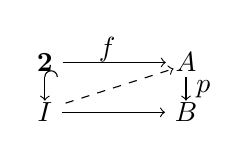
\begin{tikzpicture}[x=1.5em,y=1.5em]
  \node (tl) at (0,1.2) {$\qcTwo$};
  \node (tr) at (3.4,1.2) {$A$};
  \node (bl) at (0,0) {$\qcInt$};
  \node (br) at (3.4,0) {$B$};
  \draw[->] (tl) -- (tr);
  \node at (1.5,1.52) {$f$};
  \draw[->] (0,0.85) -- (0,0.28);
  \draw (0,0.85) arc[start angle=180,end angle=0,radius=0.15];
  \draw[->,dashed] (0.5,0.22) -- (3.1,1.05);
  \draw[->] (3.4,0.85) -- (3.4,0.28);
  \node at (3.82,0.55) {$p$};
  \draw[->] (bl) -- (br);
\end{tikzpicture}
\end{center}
\end{exercise}

\begin{exercise}\label{ex:leibniz-specialization}
将\cref{prop:leibniz-exponential}特化，以证明下列诸结论：
\begin{enumerate}[label=(\roman*)]
\item 若 $A$ 是\trQuasiCategory{}而 $X$ 是\trSimplicialSet{}，则 $A^X$ 是\trQuasiCategory{}。
\item 若 $A$ 是\trQuasiCategory{}而 $X\hookrightarrow Y$ 是\trMonomorphism{}，则
$A^Y\twoheadrightarrow A^X$ 是\trIsofibration{}。
\item 若 $A\twoheadrightarrow B$ 是\trIsofibration{}而 $X$ 是\trSimplicialSet{}，则
$A^X\twoheadrightarrow B^X$ 是\trIsofibration{}。
\end{enumerate}
\end{exercise}

\begin{exercise}\label{ex:equivalences-calculus}
预演引理 1.2.17：
\begin{enumerate}[label=(\roman*)]
\item 证明：\cref{def:equivalences-quasi-categories}所定义的\trEquivalence{}对收缩
封闭。
\item 证明：\cref{def:equivalences-quasi-categories}所定义的\trEquivalence{}满足%
\trTwoOfThreeProperty{}（2-of-3 property）。
\end{enumerate}
\end{exercise}

\begin{exercise}\label{ex:hf-surjective-equivalence}
证明：若 $f\colon X\qcTFib Y$ 是\trQuasiCategory{}之间的\trTrivialFibration{}，则\trFunctor
$\mathrm{h}f\colon\mathrm{h}X\qcEquiv\mathrm{h}Y$ 是\trCategory{}的\trSurjectiveEquivalence
（surjective equivalence）。
\end{exercise}
   %
\providecommand{\Fun}{\operatorname{Fun}}
\providecommand{\Cat}{\mathcal{C}at}
\providecommand{\sSet}{s\mathcal{S}et}
\providecommand{\QCat}{\mathcal{Q}\mathcal{C}at}
\providecommand{\CSS}{\mathcal{CSS}}
\providecommand{\rvEqArrow}{\mathrel{\stackrel{\sim}{\Rightarrow}}}
\providecommand{\rvTfibArrow}{\mathrel{\stackrel{\sim}{\twoheadrightarrow}}}
\section{\trInfinityCosmos}\label{sec:infinity-cosmos}

在 1.1 节中，我们给出了关于\trQuasiCategory{}若干基本事实的「分析的」证明。
\trQuasiCategory{}的范畴论固然可以按类似的风格发展，
但我们的目标毋宁是发展无穷维\trCategory{}的「综合的」理论，
使我们的结果能够同时适用于许多模型。为达此目的，
我们的策略不是去公理化无穷维\trCategory{}\emph{究竟是什么}，
而是去公理化它们所\emph{栖居}的范畴的「宇宙」。

\trInfinityCosmos{}的定义汲取了 1.1 节中引进的\trQuasiCategory{}\trCategory{}连同%
\trIsofibration{}、\trEquivalence{}与\trTrivialFibration{}的种种性质。%
\footnote{撇开隐喻性的典故不谈，我们的\trInfinityCosmos{}与
Street 的\trFibration{}式宇宙 \cite{bib117} 相类似。}
首先，\trQuasiCategory{}的\trCategory{}\emph{富集}于\trSimplicialSet{}的\trCategory{}之上——
从 $A$ 到 $B$ 的态射之集与\trSimplicialSet $B^A$ 的顶点之集相重合——
而且这些 hom 空间都是\trQuasiCategory{}。
其次，某些可以在\trQuasiCategory{}的非富集底范畴中定义的\trLimit{}构造
相对这种单纯富集满足泛性质，而且通常的集合\trIsomorphism{}可以扩充为\trSimplicialSet{}的\trIsomorphism{}。
最后，\trIsofibration{}、\trEquivalence{}与\trTrivialFibration{}满足一些
从抽象\trHomotopy{}论看来颇为熟悉的性质，
从而构成 Brown \cite{bib23} 意义下的\emph{\trFibration{}对象\trCategory}（见附录 C.1）。
特别地，在图表中使用\trIsofibration{}保证了它们的严格\trLimit{}是\trEquivalence{}不变的，
因此我们既能利用「到\trIsomorphism{}为止」的泛性质与这些构造的严格\trFunctor{}性，
又仍然在「\trHomotopy{}式地」工作。

正如\cref{dig:source-cosmoi-nature}中所解释的，有许多无穷维\trCategory{}的模型：
对其中的每一者，「\trInfinityCategory」（我们如此称呼它们）连同其间的「∞-\trFunctor」
所构成的\trCategory{}富集于\trQuasiCategory{}之上，
并且容许满足类似性质的\trIsofibration{}、\trEquivalence{}与\trTrivialFibration{}类。
这促成了如下的公理化。

\begin{definition}[\trInfinityCosmos]\label{def:infinity-cosmos}
一个\textbf{\trInfinityCosmos} $\mathcal{K}$
是一个富集于\trQuasiCategory{}之上的\trCategory{}，%
\footnote{这即是说 $\mathcal{K}$ 是一个\trSimpliciallyEnrichedCategory{}（见\cref{dig:simplicial-categories}），
其 hom 空间都是\trQuasiCategory{}。}
特别地，这意味着
\begin{itemize}
\item 它的态射 $f\colon A\to B$ 定义了某个\trQuasiCategory{}的顶点，
  该\trQuasiCategory{}记作 $\Fun(A,B)$，
  称为一个\textbf{\trFunctorSpace}（functor space），
\end{itemize}
而 $\mathcal{K}$ 还配备有指定的一类映射，
我们称之为\textbf{\trIsofibration{}}并记作「$\twoheadrightarrow$」，
满足以下两条公理：
\begin{enumerate}[label=(\roman*)]
\item （完备性）这个\trQuasiCategory\trEnrichedCategory $\mathcal{K}$ 拥有\trTerminal{}、小积、
  \trIsofibration{}的\trPullback{}、\trIsofibration{}的可数塔的\trLimit{}、
  以及与\trSimplicialSet{}的\trCotensor{}，
  这些\trLimit{}概念中的每一个都满足相对\trSimplicialSet{}富集的泛性质。%
  \footnote{我们在\cref{dig:simplicially-enriched-limits}中详述这些单纯富集的\trLimit{}。}
\item （\trIsofibration）\trIsofibration{}包含所有\trIsomorphism
  以及余域为\trTerminal{}的任何映射；
  在复合、积、\trPullback{}、取塔的逆\trLimit{}、
  以及与\trSimplicialSet{}的\trMonomorphism{}作 Leibniz \trCotensor{}下封闭；
  并且具有如下性质：若 $f\colon A\twoheadrightarrow B$
  是\trIsofibration{}且 $X$ 是任意对象，
  则 $\Fun(X,A)\twoheadrightarrow\Fun(X,B)$
  是\trQuasiCategory{}的\trIsofibration{}。
\end{enumerate}
\end{definition}

为便于引用，我们把 (i) 中列举的那些\trIsofibration{}图表的
单纯富集\trLimit{}统称为\textbf{\trCosmologicalLimitNotions}
（cosmological limit notions）。

\begin{definition}\label{def:equivalence-trivial-fibration}
在一个\trInfinityCosmos{}$\mathcal{K}$ 中，态射 $f\colon A\to B$ 是
\begin{itemize}
\item 一个\textbf{\trEquivalence}，当且仅当诱导映射
  $f_\ast\colon\Fun(X,A)\rvEqArrow\Fun(X,B)$
  在\trFunctorSpace{}上对一切 $X\in\mathcal{K}$
  是\trQuasiCategory{}的\trEquivalence{}，
\item 一个\textbf{\trTrivialFibration}，当且仅当 $f$
  既是\trIsofibration{}又是\trEquivalence{}。
\end{itemize}
这两个类分别记作「$\rvEqArrow$」与「$\rvTfibArrow$」。
\end{definition}

简而言之，或许可以说一个\trInfinityCosmos{}%
是一个「\trQuasiCategory{}富集的\trFibration{}对象\trCategory」
（见定义 C.1.1 与例 C.1.3）。

\begin{convention}[\trInfinityCategory{}，作为技术术语]\label{conv:infinity-category}
从此以后，我们重新把\textbf{\trInfinityCategory{}}设定为一个技术性术语，
指称任意周围\trInfinityCosmos{}中的对象。
类似地，我们用术语\textbf{∞-\trFunctor}——或者更常见地，其省略形式「\textbf{\trFunctor{}}」——
来指称\trInfinityCosmos{}中的态射 $f\colon A\to B$。
这也解释了为什么我们把\trInfinityCosmos{}中
两个\trInfinityCategory{}之间的\trQuasiCategory{} $\Fun(A,B)$
称为「\trFunctorSpace」：它的顶点正是从 $A$ 到 $B$ 的（∞-）\trFunctor{}。
\end{convention}

\begin{digression}[\trSimplicialCategory{}，附录 A.2]\label{dig:simplicial-categories}
一个\textbf{\trSimplicialCategory}（simplicial category）$\mathcal{A}$
由一些\trCategory{} $\mathcal{A}_n$ 给出：
它们带有共同的对象集，其箭头称为 $n$\textbf{-箭头}（$n$-arrows），
并且装配成一个由对象上恒等的\trFunctor{}构成的图表
$\boldsymbol{\Delta}^{op}\to\Cat$
\begin{rveq}\label{eq:simplicial-category-diagram}
\begin{tikzpicture}[xscale=0.95,yscale=1]
\node (A3) at (0,0) {$\cdots\,\mathcal{A}_3$};
\node (A2) at (4.1,0) {$\mathcal{A}_2$};
\node (A1) at (8.2,0) {$\mathcal{A}_1$};
\node (A0) at (11.9,0) {$\mathcal{A}_0$};
\node at (13.6,0) {$\coloneqq\mathcal{A}$};
\draw[->] (1.1,1.5) -- (3.1,1.5) node[midway,above]{$\scriptstyle\delta^3$};
\draw[->] (3.1,1.0) -- (1.1,1.0) node[midway,above]{$\scriptstyle\sigma^2$};
\draw[->] (1.1,0.5) -- (3.1,0.5) node[midway,above]{$\scriptstyle\delta^2$};
\draw[->] (3.1,0) -- (1.1,0) node[midway,above]{$\scriptstyle\sigma^1$};
\draw[->] (1.1,-0.5) -- (3.1,-0.5) node[midway,above]{$\scriptstyle\delta^1$};
\draw[->] (3.1,-1.0) -- (1.1,-1.0) node[midway,above]{$\scriptstyle\sigma^0$};
\draw[->] (1.1,-1.5) -- (3.1,-1.5) node[midway,above]{$\scriptstyle\delta^0$};
\draw[->] (5.2,1.0) -- (7.2,1.0) node[midway,above]{$\scriptstyle\delta^2$};
\draw[->] (7.2,0.5) -- (5.2,0.5) node[midway,above]{$\scriptstyle\sigma^1$};
\draw[->] (5.2,0) -- (7.2,0) node[midway,above]{$\scriptstyle\delta^1$};
\draw[->] (7.2,-0.5) -- (5.2,-0.5) node[midway,above]{$\scriptstyle\sigma^0$};
\draw[->] (5.2,-1.0) -- (7.2,-1.0) node[midway,above]{$\scriptstyle\delta^0$};
\draw[->] (9.3,0.5) -- (11.3,0.5) node[midway,above]{$\scriptstyle\delta^1$};
\draw[->] (11.3,0) -- (9.3,0) node[midway,above]{$\scriptstyle\sigma^0$};
\draw[->] (9.3,-0.5) -- (11.3,-0.5) node[midway,above]{$\scriptstyle\delta^0$};
\end{tikzpicture}
\end{rveq}
$0$-箭头的\trCategory{} $\mathcal{A}_0$ 是\trSimplicialCategory $\mathcal{A}$ 的
\textbf{底范畴}（underlying category），
它遗忘掉高维的单纯结构。

\trSimplicialCategory{}的数据也可以\trEquivalence{}地用一个\textbf{\trSimpliciallyEnrichedCategory}
（simplicially enriched category）来编码：
它有一个对象集，并对每一对有序对象配有态射的\trSimplicialSet $\mathcal{A}(x,y)$：
$\mathcal{A}_n$ 中从 $x$ 到 $y$ 的 $n$-箭头对应于
$\mathcal{A}(x,y)$ 中的一个 $n$-单纯形（见\cref{ex:simplicial-versus-enriched}）。
每个自同态 hom 空间都含有一个特别的恒等 $0$-箭头
（其退化像定义相应的恒等 $n$-箭头），
并且要求复合定义一个\trSimplicialMap
\begin{equation*}
\mathcal{A}(y,z)\times\mathcal{A}(x,y)
\xrightarrow{\ \circ\ }\mathcal{A}(x,z)
\end{equation*}
这一单独的映射同时编码了每个\trCategory{} $\mathcal{A}_n$ 中的复合
以及图表 \eqref{eq:simplicial-category-diagram} 的\trFunctor{}性。
复合被要求是结合且幺一的，
其含义由\trSimplicialSet{}的如下交换图表表达
\begin{equation*}
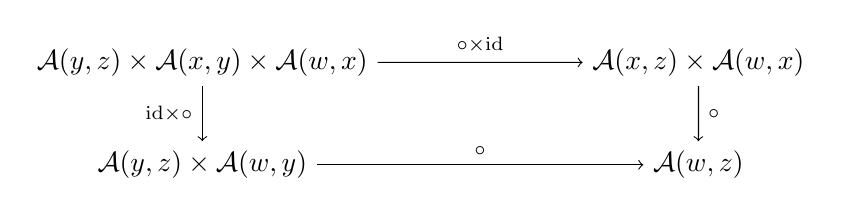
\begin{tikzpicture}[xscale=1.5,yscale=1.3]
\node (TL) at (0,1) {$\mathcal{A}(y,z)\times\mathcal{A}(x,y)\times\mathcal{A}(w,x)$};
\node (TR) at (4.2,1) {$\mathcal{A}(x,z)\times\mathcal{A}(w,x)$};
\node (BL) at (0,0) {$\mathcal{A}(y,z)\times\mathcal{A}(w,y)$};
\node (BR) at (4.2,0) {$\mathcal{A}(w,z)$};
\draw[->] (TL) -- (TR) node[midway,above]{$\scriptstyle\circ\times\mathrm{id}$};
\draw[->] (TL) -- (BL) node[midway,left]{$\scriptstyle\mathrm{id}\times\circ$};
\draw[->] (TR) -- (BR) node[midway,right]{$\scriptstyle\circ$};
\draw[->] (BL) -- (BR) node[midway,above]{$\scriptstyle\circ$};
\end{tikzpicture}
\end{equation*}
\begin{equation*}
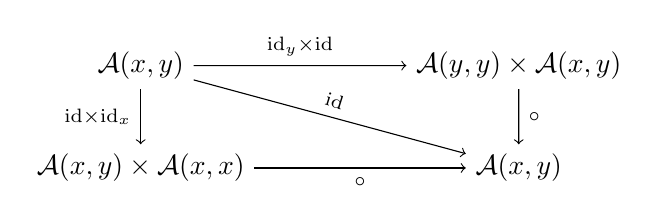
\begin{tikzpicture}[xscale=1.5,yscale=1.3]
\node (TL) at (0,1) {$\mathcal{A}(x,y)$};
\node (TR) at (3.2,1) {$\mathcal{A}(y,y)\times\mathcal{A}(x,y)$};
\node (BL) at (0,0) {$\mathcal{A}(x,y)\times\mathcal{A}(x,x)$};
\node (BR) at (3.2,0) {$\mathcal{A}(x,y)$};
\draw[->] (TL) -- (TR) node[midway,above]{$\scriptstyle\mathrm{id}_y\times\mathrm{id}$};
\draw[->] (TL) -- (BL) node[midway,left]{$\scriptstyle\mathrm{id}\times\mathrm{id}_x$};
\draw[->] (TL) -- (BR) node[midway,above,sloped]{$\scriptstyle\mathrm{id}$};
\draw[->] (TR) -- (BR) node[midway,right]{$\scriptstyle\circ$};
\draw[->] (BL) -- (BR) node[midway,below]{$\scriptstyle\circ$};
\end{tikzpicture}
\end{equation*}
由于这两种表述之间的\trEquivalence{}，
「\trSimplicialCategory」与「\trSimpliciallyEnrichedCategory」这两个术语通常被视为同义词。
\footnote{「$\Cat$ 中的单纯对象」一语保留给更一般却不那么常见的概念：
不必然由对象上恒等的\trFunctor{}构成的图表
$\boldsymbol{\Delta}^{op}\to\Cat$。}

特别地，\trInfinityCosmos{} $\mathcal{K}$ 的底范畴 $\mathcal{K}_0$
是这样的\trCategory{}：其对象是 $\mathcal{K}$ 中的\trInfinityCategory{}，
其态射是 $0$-箭头，即\trFunctorSpace{}中的顶点。
在下文将要出现的所有例子中，
这都复原出特定模型下\trInfinityCategory{}及其间\trFunctor{}的
所期望的\trCategory{}。
\end{digression}

\begin{digression}[\trSimpliciallyEnrichedLimit{}，附录 A.4–A.5]\label{dig:simplicially-enriched-limits}
设 $\mathcal{A}$ 为\trSimplicialCategory{}。对象 $A\in\mathcal{A}$
由\trSimplicialSet $U$ 作出的\textbf{\trCotensor}（cotensor）
由\trSimplicialSet{}的自然\trIsomorphism{}刻画
\begin{rveq}\label{eq:cotensor-universal}
\mathcal{A}(X,A^U)\cong\mathcal{A}(X,A)^U
\end{rveq}
假定这样的对象存在，
单纯\trCotensor{}便以唯一的方式定义一个双\trFunctor
\begin{equation*}
\begin{gathered}
\sSet^{op}\times\mathcal{A}\longrightarrow\mathcal{A}\\
(U,A)\longmapsto A^U
\end{gathered}
\end{equation*}
使得\trIsomorphism \eqref{eq:cotensor-universal} 在 $U$ 与 $A$ 上也自然。
\cref{def:infinity-cosmos}(i) 所假定的其余单纯\trLimit{}概念是\textbf{\trCone{}形的}（conical）——
这一术语用于通常的 1-范畴论\trLimit{}形状，
它们满足通常泛性质的一个富集类比（见定义 A.5.2）。
这样的\trLimit{}也定义底范畴中的\trLimit{}，但通常的泛性质被加强了。
把协变\trRepresentable{}\trFunctor
$\mathcal{A}(X,-)\colon\mathcal{A}_0\to\sSet$
用于 $\mathcal{A}_0$ 中的\trLimit{}\trCone
$(\lim_{j\in J}A_j\to A_j)_{j\in J}$，
我们得到一个自然比较映射
\begin{rveq}\label{eq:conical-comparison}
\mathcal{A}\Bigl(X,\lim_{j\in J}A_j\Bigr)
\longrightarrow\lim_{j\in J}\mathcal{A}(X,A_j).
\end{rveq}
我们说 $\lim_{j\in J}A_j$ 定义了一个\textbf{\trSimpliciallyEnrichedLimit}
（simplicially enriched limit），
当且仅当 \eqref{eq:conical-comparison}
对一切 $X\in\mathcal{A}$ 是\trSimplicialSet{}的\trIsomorphism{}。
\end{digression}

\trEnrichedCategory{}的一般理论在附录 A 中综述。

\begin{preview}[\trInfinityCosmos{}中的柔性加权\trLimit]\label{pv:flexible-weighted-limits}
\cref{def:infinity-cosmos}(i) 蕴含：任何\trInfinityCosmos{} $\mathcal{K}$
都容许所有\emph{柔性极限}（flexible limits）——
远更大的一类单纯富集的「加权」\trLimit
（见定义 6.2.1 与命题 6.2.8）。
\end{preview}

我们快速介绍三个最容易被吸收的\trInfinityCosmos{}例子，
把更精致的例子推迟到本节末尾。
其中第一个是原型性的\trInfinityCosmos{}。

\begin{proposition}[\trQuasiCategory{}的\trInfinityCosmos]\label{prop:cosmos-quasi-categories}
\trQuasiCategory{}的满子\trCategory $\QCat\subset\sSet$
定义一个\trInfinityCosmos{}，其中\trIsofibration{}、\trEquivalence{}与\trTrivialFibration{}%
恰与已具有这些名称的诸类相重合。
\end{proposition}
\begin{proof}
子\trCategory $\QCat\subset\sSet$ 的单纯富集继承自\trSimplicialSet{}的笛卡尔封闭\trCategory{}：
由命题 1.1.20，每当 $A$ 与 $B$ 是\trQuasiCategory{}， %
$\Fun(A,B):=B^A$ 仍是\trQuasiCategory{}。
\cref{def:infinity-cosmos}(i) 中假定的宇宙论\trLimit{}存在于周围的\trSimplicialSet\trCategory{}中。%
\footnote{任何预层\trCategory{}都是笛卡尔封闭、完备且余完备的——
Bénabou 意义下的一个「宇宙」。}
例如，单纯\trCotensor \eqref{eq:cotensor-universal} 的定义性泛性质
由\trSimplicialSet{}的指数满足。此外，由于\trSimplicialSet{}的\trCategory{}是\trCartesianClosed{}，
每个\trCone{}形\trLimit{}都在\cref{dig:simplicially-enriched-limits}所讨论的意义下单纯富集
（见\cref{ex:conical-products-qcat}与命题 A.5.4）。

我们现在论证\trQuasiCategory{}的满子\trCategory{}继承所有这些\trLimit{}概念，
同时建立\trIsofibration{}在这些\trLimit{}的构造下的稳定性。
事实上，后一性质有助于证明前一性质。
为看到这一点，注意\trSimplicialSet{}是\trQuasiCategory{}，当且仅当
从它到点的映射是\trIsofibration{}。
更一般地，若任何\trIsofibration{}的余域是\trQuasiCategory{}，
则其定义域也必是。
于是，若\trQuasiCategory{}图表上的\trLimit{}\trCone{}中只要有映射是\trIsofibration{}，
便可推出该\trLimit{}本身是\trQuasiCategory{}。

由于\trIsofibration{}由右提升性质刻画，
引理 C.2.3 蕴含\trIsofibration{}包含所有\trIsomorphism{}，
并且在复合、积、\trPullback{}与取塔的逆\trLimit{}下封闭。
特别地，\trQuasiCategory{}的满子\trCategory{}拥有这些\trLimit{}。
这就验证了 \cref{def:infinity-cosmos}(i) 与 (ii) 的全部公理，
除了最后两条：Leibniz 封闭性与对取指数 $(-)^X$ 的封闭性。
这最后的封闭性质已在命题 1.1.20 中建立， %
而且事实上由练习 1.1.vii，前者涵盖后者。
这就完成了对\trInfinityCosmos{}公理的验证。

剩下要检查的是\trEquivalence{}与\trTrivialFibration
恰与 1.1.23 及 1.1.25 所定义的映射重合。 %
由命题 1.1.28，后一重合由前一重合推出， %
故只剩下证明 1.1.23 的\trEquivalence{}与 %
\textbf{可表示地定义的\trEquivalence}（representably defined equivalences）
重合：即那些使 $A^X\to B^X$ 成为定义 1.1.23 意义下\trQuasiCategory{}的%
\trEquivalence{}的%
\trQuasiCategory{}映射 $f\colon A\to B$。
取 $X=\Delta[0]$，立即可见可表示地定义的\trEquivalence{}是\trEquivalence{}，
而逆命题成立，因为指数 $(-)^X$
保持定义单纯\trHomotopy{}的数据。
\end{proof}

另外两个例子符合同一范式：
二者都作为\trQuasiCategory{}的\trInfinityCosmos{}的满子\trCategory{}出现，
并从这个包含继承其\trInfinityCosmos{}结构（见引理 6.1.4）。
但描述所得到的\trInfinityCosmos{}结构本身也富有教益，
而且归根结底工作量更小。

\begin{proposition}[\trCategory{}的\trInfinityCosmos]\label{prop:cosmos-categories}
1-\trCategory{}的\trCategory{} $\Cat$
定义一个\trInfinityCosmos{}，其\trIsofibration{}恰是
\textbf{\trIsofibration}：即满足下图所示右提升性质的\trFunctor
\begin{center}
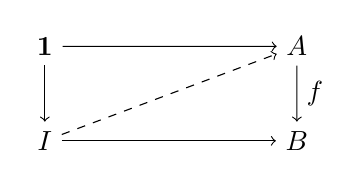
\begin{tikzpicture}[xscale=1.6,yscale=1.2]
\node (TL) at (0,1) {$\mathbf{1}$};
\node (TR) at (2,1) {$A$};
\node (BL) at (0,0) {$\mathbb{I}$};
\node (BR) at (2,0) {$B$};
\draw[->] (TL) -- (TR);
\draw[->] (TL) -- (BL);
\draw[->] (BL) -- (BR);
\draw[->] (TR) -- (BR) node[midway,right]{$f$};
\draw[dashed,->] (BL) -- (TR);
\end{tikzpicture}
\end{center}
\trEquivalence{}恰是\trCategory{}的\trEquivalence{}，而\trTrivialFibration{}恰是
\textbf{满射\trEquivalence}（surjective equivalences）：
在对象上也为满射的\trCategory\trEquivalence{}。
\end{proposition}
\begin{proof}
众所周知，\trCategory{}的 2-\trCategory{}作为 $\Cat$-富集的\trCategory{}是完备的
（其实也余完备）（见定义 A.6.17 或文献 \cite{bib67}）。
把\trNerve\trFunctor{}用于 hom-\trCategory{}，
\trCategory{}的这个\trEnrichedCategory{}便成为\trQuasiCategory\trEnrichedCategory{}（见附录 A.7）。
由于\trNerve\trFunctor{}是右\trAdjunction{}，
这些 2-范畴论的\trLimit{}在形式上变成单纯富集\trLimit{}。
特别地，如命题 A.7.8 所规定的，
\trCategory{} $A$ 由\trSimplicialSet $U$ 作出的\trCotensor
定义为\trFunctor{}\trCategory $A^{hU}$。
这就完成了公理 (i) 的验证。

由于\trIsofibration{}的类由右提升性质刻画，
引理 C.2.3 蕴含\trIsofibration{}对 \cref{def:infinity-cosmos}(ii)
除最后两条之外的所有\trLimit{}构造封闭；
而由练习 1.1.vii，Leibniz 封闭性涵盖对取指数的封闭性。

要验证\trCategory{}的\trIsofibration{} $f\colon A\twoheadrightarrow B$
在与\trSimplicialSet{}的\trMonomorphism $i\colon U\hookrightarrow V$
作 Leibniz \trCotensor{}下的稳定性，
我们必须求解左下的\trLifting{}问题
\begin{equation*}
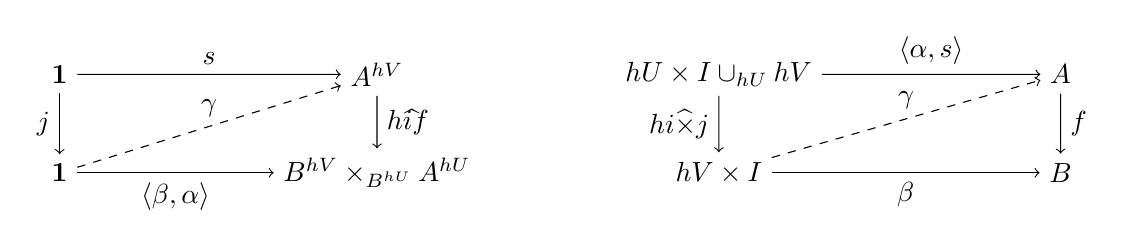
\begin{tikzpicture}[xscale=1.55,yscale=1.25]
\node (TL) at (0,1) {$\mathbf{1}$};
\node (TR) at (2.6,1) {$A^{hV}$};
\node (BL) at (0,0) {$\mathbf{1}$};
\node (BR) at (2.6,0) {$B^{hV}\times_{B^{hU}}A^{hU}$};
\draw[->] (TL) -- (TR) node[midway,above]{$s$};
\draw[->] (TL) -- (BL) node[midway,left]{$j$};
\draw[->] (BL) -- (BR) node[midway,below]{$\langle\beta,\alpha\rangle$};
\draw[->] (TR) -- (BR) node[midway,right]{$hi\widehat{\pitchfork}f$};
\draw[dashed,->] (BL) -- (TR) node[midway,above]{$\gamma$};
\node at (4.15,0.5) {$\leftrightsquigarrow$};
\node (rTL) at (5.4,1) {$hU\times\mathbb{I}\cup_{hU}hV$};
\node (rTR) at (8.2,1) {$A$};
\node (rBL) at (5.4,0) {$hV\times\mathbb{I}$};
\node (rBR) at (8.2,0) {$B$};
\draw[->] (rTL) -- (rTR) node[midway,above]{$\langle\alpha,s\rangle$};
\draw[->] (rTL) -- (rBL) node[midway,left]{$hi\widehat{\times}j$};
\draw[->] (rBL) -- (rBR) node[midway,below]{$\beta$};
\draw[->] (rTR) -- (rBR) node[midway,right]{$f$};
\draw[dashed,->] (rBL) -- (rTR) node[midway,above]{$\gamma$};
\end{tikzpicture}
\end{equation*}
它转置为右上的\trLifting{}问题，而后者可以手工求解。
这里映射 $\beta$ 定义了 $fs\colon hV\to B$
与另一个\trFunctor{}之间的自然\trIsomorphism{}。
我们的任务是把它\trLifting{}为从 $s$ 到另一\trFunctor{}的自然\trIsomorphism $\gamma$，
使 $\gamma$ 沿 $hi\colon hU\to hV$ 延拓自然\trIsomorphism $\alpha$。
注意\trFunctor{} $hi$ 未必是包含，
但它在对象上单射，这就够了。

我们分情形定义 $\gamma$ 的分量。
若对象 $v\in hV$ 等于某个 $u\in hU$ 的像 $i(u)$，
则定义 $\gamma_{i(u)}:=\alpha_u$；
否则，利用 $f$ 是\trIsofibration{}这一事实，
把\trIsomorphism $\beta_v$ \trLifting{}为 $A$ 中以 $s(v)$ 为定义域的\trIsomorphism{}，从而定义 $\gamma_v$。
映射 $\gamma\colon hV\times\mathbb{I}\to A$ 的数据
还蕴含指定作为自然\trIsomorphism $\gamma$ 之余域的\trFunctor{} $hV\to A$。
在对象上，该\trFunctor{}由 $v\mapsto\mathrm{cod}(\gamma_v)$ 给出；
在态射上，它以唯一的方式定义，使得 $\gamma$ 成为\trNaturalTransformation
\begin{equation*}
(k\colon v\to v^{\prime})\mapsto
\gamma_{v^{\prime}}\circ s(k)\circ\gamma_v^{-1}.
\end{equation*}
这就完成了 $\Cat$ 定义一个\trInfinityCosmos{}的证明。
由于\trFunctor{}\trCategory{}（如 $A^{\mathbb{I}}$）的\trNerve
\trIsomorphism{}于其\trNerve{}之间的指数，
\trCategory{}的\trEquivalence{}恰与定义 1.1.23 的\trEquivalence{}重合。 %
于是\trCategory{}的\trInfinityCosmos{}中的\trEquivalence{}%
恰与\trCategory{}的\trEquivalence{}重合，
而由于满射\trEquivalence{}是\trEquivalence{}与\trIsofibration{}之交，
证明完毕。
\end{proof}

\begin{proposition}[\trKanComplex{}的\trInfinityCosmos]\label{prop:cosmos-kan-complexes}
\trKanComplex{}的\trCategory{} $\mathcal{K}an$
定义一个\trInfinityCosmos{}，其\trIsofibration{}恰是
\textbf{\trKanFibration}（Kan fibrations）：
即对所有 $n\geq 1$ 与 $0\leq k\leq n$
对一切\trHorn{}包含 $\Lambda^k[n]\hookrightarrow\Delta[n]$ 可\trLifting{}的映射。
\end{proposition}
其证明沿引理 6.1.4 的路线进行。
我们证明\trKanComplex{}的子\trCategory
通过从\trQuasiCategory{}的\trInfinityCosmos{}限制结构
而继承一个\trInfinityCosmos{}结构。
\begin{proof}
由命题 1.1.18，\trKanComplex{}之间的\trIsofibration{}是\trKanFibration{}。 %
反之，由于\trHomotopyCoherentIsomorphism $\mathbb{I}$
可以从点 $\mathbf{1}$ 出发、通过对外\trHorn{}逐个贴上填充物而构造出来，
所有\trKanFibration{}都定义\trIsofibration{}。
这表明\trKanComplex{}之间\trIsofibration{}与\trKanFibration{}重合。
于是，为证明\trKanComplex{}的\trCategory{}通过从\trQuasiCategory{}的%
\trInfinityCosmos{}限制而继承\trInfinityCosmos{}结构，
我们只需验证满子\trCategory $\mathcal{K}an\hookrightarrow\QCat$
对 \cref{def:infinity-cosmos}(i) 的所有\trLimit{}构造封闭。
对\trCone{}形\trLimit{}，论证与\cref{prop:cosmos-quasi-categories}之证明所给的论证互为镜像；
而对\trCotensor{}的封闭性则是推论 D.3.11 的推论， %
后者蕴含\trKanComplex{}在\trSimplicialSet{}的\trCategory{}中也定义一个\trExponentialIdeal{}。
其余公理，即 \cref{def:infinity-cosmos}(ii)，则从\cref{prop:cosmos-quasi-categories}中
对\trQuasiCategory{}建立的类似性质继承而来。
\end{proof}

我们对熟悉 Quillen \trModelCategory——抽象\trHomotopy{}论的一个流行框架——的读者，
提及一个自然界中\trInfinityCosmos{}的共同来源以建立直观；
同时也让新来者放心：在证明这些结果的附录 E 之外，
并不需要\trModelCategory{}。

\begin{digression}[自然界中\trInfinityCosmos{}的一个来源]\label{dig:source-cosmoi-nature}
如附录 E.1 中所解释的，
\trModelCategory{}的某些易于描述的性质蕴含：
\trFibration{}对象的满子\trCategory{}定义一个\trInfinityCosmos{}，
其\trIsofibration{}、\trEquivalence{}与\trTrivialFibration
恰是\trFibration{}对象之间的\trFibration{}、弱\trEquivalence{}与\trTrivialFibration{}。
也就是说，任何\trModelCategory{}，
只要它如此富集于\trSimplicialSet{}的 Joyal \trModelStructure{}之上、
且其中所有\trFibration{}对象都是余\trFibration{}的，
就呈现一个\trInfinityCosmos{}（见命题 E.1.1）。
这种对\trQuasiCategory{}的模型范畴论式富集
可以在\trModelCategory{}为笛卡尔封闭、
且配备有到\trSimplicialSet{}的 Joyal \trModelStructure{}的右 Quillen \trAdjunction{}、
其左\trAdjunction{}保持有限积时定义（见推论 E.1.4）。
此时，右\trAdjunction{}成为底\trQuasiCategory\trFunctor
（见命题 1.3.4(ii)）， %
而且如此产生的诸\trInfinityCosmos{}是\trCartesianClosed
（见\cref{def:cartesian-closed-cosmoi}）。
\cref{exa:cosmoi-models}中列出的诸\trInfinityCosmos{}全都以这种方式产生。
\end{digression}

下列结果是定义 1.2.1 的公理的推论。
首先，观察到\trTrivialFibration
享有与\trIsofibration{}相同的稳定性性质。

\begin{lemma}[\trTrivialFibration{}的稳定性]\label{lem:trivial-fibration-stability}
\trInfinityCosmos{}中的\trTrivialFibration{}定义一个包含所有\trIsomorphism{}的子\trCategory{}，
并且在积、\trPullback{}与取塔的逆\trLimit{}下稳定。
此外，任何\trTrivialFibration{}与\trSimplicialSet{}\trMonomorphism{}的 Leibniz \trCotensor{}是\trTrivialFibration{}， %
\trIsofibration{}与由内\trHorn{}包含及映射
$\mathbf{1}\hookrightarrow\mathbb{I}$
\trCell{}式生成的类中映射的 Leibniz \trCotensor{}亦然；
且若 $E\rvTfibArrow B$ 是\trTrivialFibration{}，
则 $\Fun(X,E)\rvTfibArrow\Fun(X,B)$ 亦然。
\end{lemma}
\begin{proof}
我们按相反的顺序证明这些陈述。
由 \cref{def:infinity-cosmos}(ii) 及\trInfinityCosmos{}中\trTrivialFibration{}的定义，我们知道：
若 $E\rvTfibArrow B$ 是\trTrivialFibration{}，
则 $\Fun(X,E)\rvTfibArrow\Fun(X,B)$
既是\trIsofibration{}又是\trEquivalence{}，
从而由命题 1.1.28 是\trTrivialFibration{}。 %
对其余构造的稳定性，
我们在每种情形都知道所涉映射是\trInfinityCosmos{}中的\trIsofibration{}；
剩下的只是证明这些映射也是\trEquivalence{}。
\trInfinityCosmos{}中的\trEquivalence{}%
被定义为被 $\Fun(X,-)$ 载为\trQuasiCategory{}之\trEquivalence{}的那些映射，
故只需验证\trQuasiCategory{}的\trTrivialFibration{}满足相应的稳定性性质。
对 Leibniz 稳定性性质，这已在命题 1.1.29 中建立，
而其余性质由引理 C.2.3 覆盖。
\end{proof}

由一个 Yoneda 式的论证，
定义 1.1.23 中\trQuasiCategory{}的\trInfinityCosmos{}的%
\trEquivalence{}的「\trHomotopyEquivalence」刻画，
可以扩充为任何\trInfinityCosmos{}中\trEquivalence{}的类似刻画：

\begin{lemma}[\trEquivalence{}是\trHomotopyEquivalence]\label{lem:equiv-homotopy-equivalences}
\trInfinityCosmos{} $\mathcal{K}$ 中\trInfinityCategory{}之间的
映射 $f\colon A\to B$ 是\trEquivalence{}，当且仅当
它扩充为「\trHomotopyEquivalence」的数据，
并以\trFreeLivingIsomorphism $\mathbb{I}$ 作为区间：
也就是说，若存在映射 $g\colon B\to A$
\begin{rveq}\label{eq:homotopy-equivalence-data}
\begin{tikzpicture}[xscale=1.35,yscale=1.05]
\node (lA) at (0,0) {$A$};
\node (tA) at (2.2,1.3) {$A$};
\node (Ai) at (2.2,0) {$A^{\mathbb{I}}$};
\node (bA) at (2.2,-1.3) {$A$};
\draw[double] (lA) -- (tA);
\draw[->] (Ai) -- (tA) node[midway,right]{$\mathrm{ev}_0$};
\draw[->] (lA) -- (Ai) node[midway,above]{$\alpha$};
\draw[->] (lA) -- (bA) node[midway,below]{$gf$};
\draw[->] (Ai) -- (bA) node[midway,right]{$\mathrm{ev}_1$};
\node at (4.1,0) {及};
\node (lB) at (6,0) {$B$};
\node (tB) at (8.2,1.3) {$B$};
\node (Bi) at (8.2,0) {$B^{\mathbb{I}}$};
\node (bB) at (8.2,-1.3) {$B$};
\draw[->] (lB) -- (tB) node[midway,above]{$fg$};
\draw[->] (Bi) -- (tB) node[midway,right]{$\mathrm{ev}_0$};
\draw[->] (lB) -- (Bi) node[midway,above]{$\beta$};
\draw[double] (lB) -- (bB);
\draw[->] (Bi) -- (bB) node[midway,right]{$\mathrm{ev}_1$};
\end{tikzpicture}
\end{rveq}
在\trInfinityCosmos{}之中。
\end{lemma}
\begin{proof}
按假设，若 $f\colon A\to B$ 定义\trInfinityCosmos{} $\mathcal{K}$
中的\trEquivalence{}，
则复合后诱导的映射 $f_\ast\colon\Fun(B,A)\rvEqArrow\Fun(B,B)$
是定义 1.1.23 意义下\trQuasiCategory{}的\trEquivalence{}。 %
在 $0$-箭头 $\mathrm{id}_B\in\Fun(B,B)$ 处
取值于逆\trEquivalence{} $\tilde{g}\colon\Fun(B,B)\rvEqArrow\Fun(B,A)$
与\trHomotopy $\tilde{\beta}\colon\Fun(B,B)\to\Fun(B,B)^{\mathbb{I}}$，
我们得到 $0$-箭头 $g\colon B\to A$，
连同从复合 $fg$ 到 $\mathrm{id}_B$
的\trIsomorphism $\beta\colon\mathbb{I}\to\Fun(B,B)$。
由\trCotensor \eqref{eq:cotensor-universal} 的定义性泛性质，
这一\trIsomorphism{}内部化而定义 $\mathcal{K}$ 中的映射
$\beta\colon B\to B^{\mathbb{I}}$，
即 \eqref{eq:homotopy-equivalence-data} 右侧所示者。

现在，$f$ 是\trEquivalence{}这一假设还提供%
\trQuasiCategory{}的\trEquivalence{} $f_\ast\colon\Fun(A,A)\rvEqArrow\Fun(A,B)$，
而映射 $\beta f\colon A\to B^{\mathbb{I}}$
表示 $\Fun(A,B)$ 中从 $fgf$ 到 $f$ 的\trIsomorphism{}。
由于 $f_\ast$ 是\trEquivalence{}，
我们从注 1.1.24 得出 $\mathrm{id}_A$ 与 $gf$
在\trQuasiCategory $\Fun(A,A)$ 中\trIsomorphism{}：
显式地，这样的\trIsomorphism{}可以这样定义——
取逆\trEquivalence{} $\tilde{h}\colon\Fun(A,B)\to\Fun(A,A)$，
并与从 $\mathrm{id}_{\Fun(A,A)}$ 到 $\tilde{h}f_\ast$
的\trIsomorphism $\tilde{\alpha}\colon\Fun(A,A)\to\Fun(A,A)^{\mathbb{I}}$
在 $\mathrm{id}_A$ 与 $gf\in\Fun(A,A)$ 处的分量作复合。
现在由推论 1.1.16，
这一\trIsomorphism{}由从 $\mathrm{id}_A$ 到 $gf$ 的映射
$\mathbb{I}\to\Fun(A,A)$ 表示，
后者内部化为 $\mathcal{K}$ 中的映射 $\alpha\colon A\to A^{\mathbb{I}}$，
即 \eqref{eq:homotopy-equivalence-data} 左侧所示者。

逆命题容易：
单纯\trCotensor{}构造与 $\Fun(X,-)$ 交换，
故\trHomotopyEquivalence \eqref{eq:homotopy-equivalence-data} 诱导
定义 1.1.23 意义下\trQuasiCategory{}的\trHomotopyEquivalence{}。 %
\end{proof}

\begin{lemma}\label{lem:equivalence-retracts-2-of-3}
\trInfinityCosmos{}中的\trEquivalence{}对收缩封闭，
并满足\textbf{\trTwoOfThreeProperty}（2-of-3 property）：
给定可复合的一对\trFunctor{}及其复合，
若其中任何两个是\trEquivalence{}，则第三个亦然。
\end{lemma}
由\trEquivalence{}的可表示定义与\trFunctor{}性，
\cref{lem:equivalence-retracts-2-of-3} 从\trQuasiCategory{}之间%
\trEquivalence{}的相应结果
（见练习 1.1.viii）容易推出。
但为完备起见，
我们不依赖这一基础情形而证明一般的宇宙论结果，
从而涵盖练习 1.1.viii。
\begin{proof}
设 $f\colon A\rvEqArrow B$ 是配有
\eqref{eq:homotopy-equivalence-data} 之数据的\trEquivalence{}，
并考虑收缩图表
\begin{center}
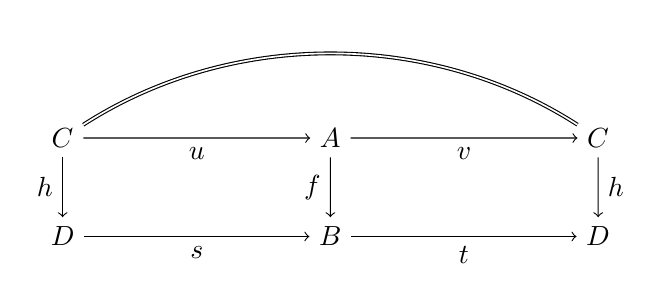
\begin{tikzpicture}[xscale=1.7,yscale=1.25]
\node (CL) at (0,1) {$C$};
\node (A) at (2,1) {$A$};
\node (CR) at (4,1) {$C$};
\node (DL) at (0,0) {$D$};
\node (B) at (2,0) {$B$};
\node (DR) at (4,0) {$D$};
\draw[double] (CL) to[out=40,in=140] (CR);
\draw[->] (CL) -- (A) node[midway,below]{$u$};
\draw[->] (A) -- (CR) node[midway,below]{$v$};
\draw[->] (CL) -- (DL) node[midway,left]{$h$};
\draw[->] (A) -- (B) node[midway,left]{$f$};
\draw[->] (CR) -- (DR) node[midway,right]{$h$};
\draw[->] (DL) -- (B) node[midway,below]{$s$};
\draw[->] (B) -- (DR) node[midway,below]{$t$};
\end{tikzpicture}
\end{center}
由\cref{lem:equiv-homotopy-equivalences}，要证 $h\colon C\to D$ 是\trEquivalence{}，
只需构造逆\trHomotopyEquivalence{}的数据。
为此定义 $k\colon D\to C$ 为复合 $vgs$，
然后从交换图表
\begin{center}
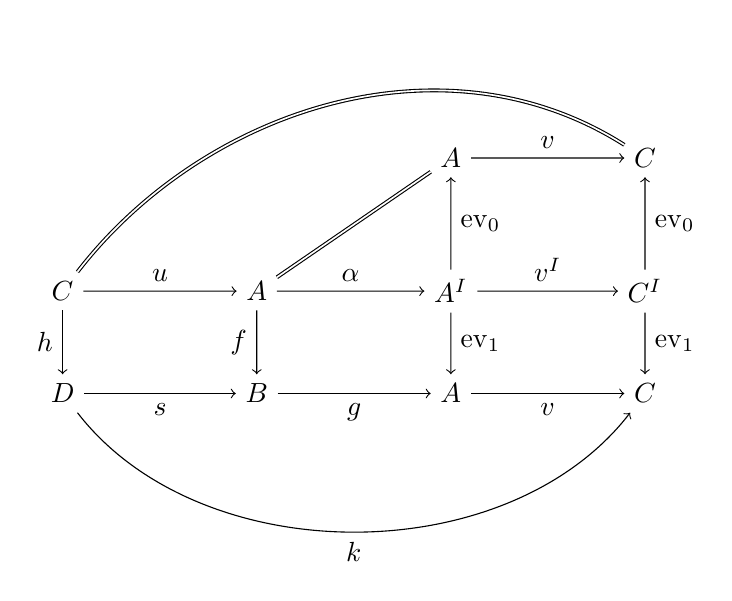
\begin{tikzpicture}[xscale=1.45,yscale=1.3]
\node (Cm) at (0,1) {$C$};
\node (A2) at (1.7,1) {$A$};
\node (Ai) at (3.4,1) {$A^{\mathbb{I}}$};
\node (Ci) at (5.1,1) {$C^{\mathbb{I}}$};
\node (At) at (3.4,2.3) {$A$};
\node (Ct) at (5.1,2.3) {$C$};
\node (D) at (0,0) {$D$};
\node (B) at (1.7,0) {$B$};
\node (Ab) at (3.4,0) {$A$};
\node (Cb) at (5.1,0) {$C$};
\draw[double] (Cm) to[out=55,in=145] (Ct);
\draw[->] (At) -- (Ct) node[midway,above]{$v$};
\draw[double] (A2) -- (At);
\draw[->] (Cm) -- (A2) node[midway,above]{$u$};
\draw[->] (A2) -- (Ai) node[midway,above]{$\alpha$};
\draw[->] (Ai) -- (Ci) node[midway,above]{$v^{\mathbb{I}}$};
\draw[->] (Ai) -- (At) node[midway,right]{$\mathrm{ev}_0$};
\draw[->] (Ci) -- (Ct) node[midway,right]{$\mathrm{ev}_0$};
\draw[->] (Ai) -- (Ab) node[midway,right]{$\mathrm{ev}_1$};
\draw[->] (Ci) -- (Cb) node[midway,right]{$\mathrm{ev}_1$};
\draw[->] (Cm) -- (D) node[midway,left]{$h$};
\draw[->] (A2) -- (B) node[midway,left]{$f$};
\draw[->] (D) -- (B) node[midway,below]{$s$};
\draw[->] (B) -- (Ab) node[midway,below]{$g$};
\draw[->] (Ab) -- (Cb) node[midway,below]{$v$};
\draw[->] (D) to[out=-55,in=-125] node[midway,below]{$k$} (Cb);
\end{tikzpicture}
\end{center}
\begin{center}
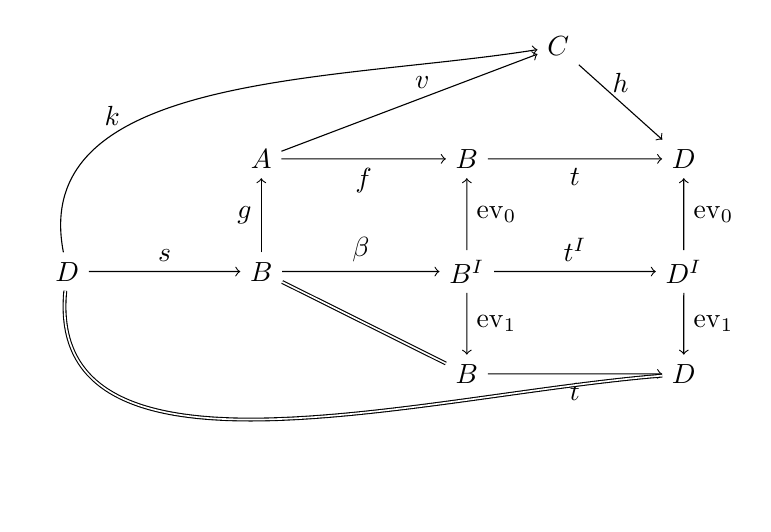
\begin{tikzpicture}[xscale=1.45,yscale=1.3]
\node (C) at (2.6,2.7) {$C$};
\node (A) at (0,1.6) {$A$};
\node (B) at (1.8,1.6) {$B$};
\node (D) at (3.7,1.6) {$D$};
\node (Dr) at (-1.7,0.5) {$D$};
\node (B3) at (0,0.5) {$B$};
\node (Bi) at (1.8,0.5) {$B^{\mathbb{I}}$};
\node (Di) at (3.7,0.5) {$D^{\mathbb{I}}$};
\node (Bb) at (1.8,-0.5) {$B$};
\node (Db) at (3.7,-0.5) {$D$};
\draw[->] (Dr) to[out=100,in=190] node[pos=0.3,above]{$k$} (C);
\draw[->] (A) -- (C) node[pos=0.55,above]{$v$};
\draw[->] (C) -- (D) node[midway,above]{$h$};
\draw[->] (A) -- (B) node[midway,below]{$f$};
\draw[->] (B) -- (D) node[midway,below]{$t$};
\draw[->] (B3) -- (A) node[midway,left]{$g$};
\draw[->] (Bi) -- (B) node[midway,right]{$\mathrm{ev}_0$};
\draw[->] (Di) -- (D) node[midway,right]{$\mathrm{ev}_0$};
\draw[->] (Dr) -- (B3) node[midway,above]{$s$};
\draw[->] (B3) -- (Bi) node[midway,above]{$\beta$};
\draw[->] (Bi) -- (Di) node[midway,above]{$t^{\mathbb{I}}$};
\draw[->] (Bi) -- (Bb) node[midway,right]{$\mathrm{ev}_1$};
\draw[->] (Di) -- (Db) node[midway,right]{$\mathrm{ev}_1$};
\draw[->] (Bb) -- (Db) node[midway,below]{$t$};
\draw[double] (B3) -- (Bb);
\draw[double] (Dr) to[out=-95,in=185] (Db);
\end{tikzpicture}
\end{center}
观察到 $v^{\mathbb{I}}\alpha u\colon C\to C^{\mathbb{I}}$
与 $t^{\mathbb{I}}\beta s\colon D\to D^{\mathbb{I}}$
定义了所需的\trHomotopyCoherentIsomorphism{}。

经由\cref{lem:equiv-homotopy-equivalences}，
\trEquivalence{}的\trTwoOfThreeProperty{}从%
\trQuasiCategory{}中\trIsomorphism{}之集对复合封闭这一事实推出。
\trQuasiCategory{}中的\trHomotopyCoherentIsomorphism{}表示\trHomotopyCategory{}中的\trIsomorphism{}，
其在\trHomotopyCategory{}中的复合是\trIsomorphism{}，
而由推论 1.1.16，
它可以被\trLifting{}为表示它的\trHomotopyCoherentIsomorphism{}。%
\footnote{事实上，由例 D.5.5，
\trHomotopyCoherentIsomorphism{}可以直接复合，但这里不需要这一点。}
现在我们把它用于\trInfinityCosmos{}的\trFunctorSpace{}中、
构成\trInfinityCategory{}之\trEquivalence{}数据一部分的
那些\trHomotopyCoherentIsomorphism{}。

要证\trEquivalence{}对复合封闭，
考虑一对可复合的\trEquivalence{}及其逆\trEquivalence
\begin{center}
\begin{tikzpicture}[xscale=1.7,yscale=1.1]
\node (A) at (0,0.6) {$A$};
\node (B) at (2,0.6) {$B$};
\node (C) at (4,0.6) {$C$};
\node (A2) at (0,-0.6) {$A$};
\node (B2) at (2,-0.6) {$B$};
\node (C2) at (4,-0.6) {$C$};
\draw[->] (A) -- (B) node[above]{$\overset{\simeq}{f}$};
\draw[->] (B) -- (C) node[above]{$\overset{\simeq}{g}$};
\draw[->] (B2) -- (A2) node[above]{$\overset{\simeq}{k}$};
\draw[->] (C2) -- (B2) node[above]{$\overset{\simeq}{h}$};
\end{tikzpicture}
\end{center}
\cref{lem:equiv-homotopy-equivalences} 的\trEquivalence{}数据定义\trIsomorphism
$\alpha\colon\mathrm{id}_A\cong kf\in\Fun(A,A)$
与 $\gamma\colon\mathrm{id}_B\cong hg\in\Fun(B,B)$，
后者经须状复合定义
$k\gamma f\colon kf\cong khgf\in\Fun(A,A)$。%
\yizhu{原书印作「$\Fun(B,B)$」，疑为「$\Fun(A,A)$」之误，此处径改。}
复合这两者，我们得到\trIsomorphism
$\mathrm{id}_A\cong khgf\in\Fun(A,A)$，
见证 $kh$ 定义 $gf$ 的左\trEquivalence{}逆。
另一\trIsomorphism{}类似地构造。

要证\trEquivalence{}对右消去封闭，考虑图表
\begin{center}
\begin{tikzpicture}[xscale=1.7,yscale=1.1]
\node (A) at (0,0) {$A$};
\node (B) at (2,0) {$B$};
\node (C) at (4,0) {$C$};
\draw[->] (C) to[out=140,in=40] node[above]{$\overset{\simeq}{\ell}$} (A);
\draw[->] (A) -- (B) node[above]{$\overset{\simeq}{f}$};
\draw[->] (B) -- (C) node[above]{$g$};
\draw[->] (B) -- (A) node[below]{$\overset{\simeq}{k}$};
\end{tikzpicture}
\end{center}
其中 $k$ 是 $f$ 的逆\trEquivalence{}，
而 $\ell$ 是 $gf$ 的逆\trEquivalence{}。
我们断言 $f\ell$ 定义 $g$ 的逆\trEquivalence{}。
所需的\trIsomorphism $\mathrm{id}_C\cong gf\ell$ 之一已经给出；
另一个通过复合 $\Fun(B,B)$ 中的三个\trIsomorphism{}得到
\begin{equation*}
\mathrm{id}_B
\xrightarrow[\ \beta^{-1}\ ]{\ \simeq\ }fk
\xrightarrow[\ f\delta k\ ]{\ \simeq\ }f\ell gfk
\xrightarrow[\ f\ell g\beta\ ]{\ \simeq\ }f\ell g.
\end{equation*}
\trEquivalence{}对左消去的稳定性之证明是对偶的。
\end{proof}

\trTrivialFibration{}容许一个类似的刻画，即作为\trSplitFiberHomotopyEquivalence{}。

\begin{lemma}[\trTrivialFibration{}分裂]\label{lem:trivial-fibrations-split}
每个\trTrivialFibration{}容许一个截面
\begin{center}
\begin{tikzpicture}[xscale=1.5,yscale=1.2]
\node (E) at (1.5,1.1) {$E$};
\node (BL) at (0,0) {$B$};
\node (BR) at (3,0) {$B$};
\draw[dashed,->] (BL) -- (E) node[pos=0.35,above,sloped]{$s$};
\draw[->] (E) -- (BR) node[midway,right]{$\overset{\simeq}{p}$};
\draw[double] (BL) -- (BR);
\end{tikzpicture}
\end{center}
该截面定义一个\trSplitFiberHomotopyEquivalence
\begin{center}
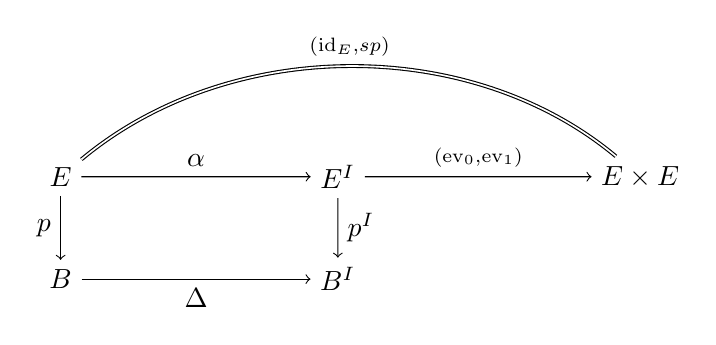
\begin{tikzpicture}[xscale=1.6,yscale=1.3]
\node (E) at (0,1) {$E$};
\node (Ei) at (2.2,1) {$E^{\mathbb{I}}$};
\node (EE) at (4.6,1) {$E\times E$};
\node (B) at (0,0) {$B$};
\node (Bi) at (2.2,0) {$B^{\mathbb{I}}$};
\draw[->] (E) -- (Ei) node[midway,above]{$\alpha$};
\draw[double] (E) to[out=45,in=135] node[midway,above]{$\scriptstyle(\mathrm{id}_E,sp)$} (EE);
\draw[->] (Ei) -- (EE) node[midway,above]{$\scriptstyle(\mathrm{ev}_0,\mathrm{ev}_1)$};
\draw[->] (E) -- (B) node[midway,left]{$p$};
\draw[->] (Ei) -- (Bi) node[midway,right]{$p^{\mathbb{I}}$};
\draw[->] (B) -- (Bi) node[midway,below]{$\Delta$};
\end{tikzpicture}
\end{center}
反之，任何定义\trSplitFiberHomotopyEquivalence{}的\trIsofibration{}%
是\trTrivialFibration{}。
\end{lemma}
\begin{proof}
若 $p\colon E\rvTfibArrow B$ 是\trTrivialFibration{}，
则由\cref{lem:trivial-fibration-stability}的末条稳定性性质，
对任意\trInfinityCategory{} $X$，
$p_\ast\colon\Fun(X,E)\rvTfibArrow\Fun(X,B)$ 亦然。
由定义 1.1.25，我们可以求解左下的\trLifting{}问题 %
\begin{equation*}
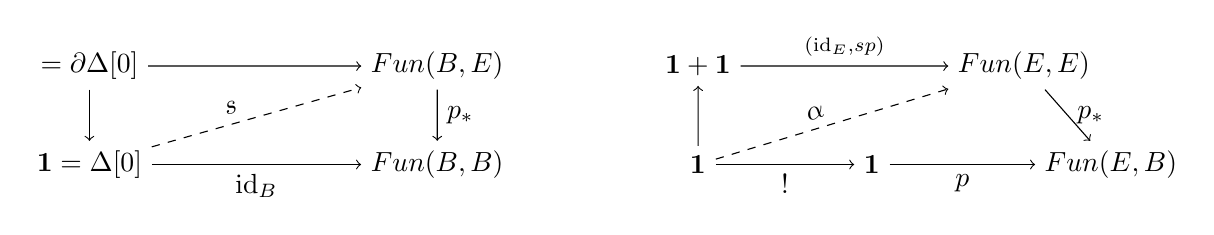
\begin{tikzpicture}[xscale=1.38,yscale=1.25]
\node (TL) at (0,1) {$\varnothing=\partial\Delta[0]$};
\node (TR) at (3.2,1) {$\Fun(B,E)$};
\node (BL) at (0,0) {$\mathbf{1}=\Delta[0]$};
\node (BR) at (3.2,0) {$\Fun(B,B)$};
\draw[->] (TL) -- (TR);
\draw[->] (TL) -- (BL);
\draw[->] (BL) -- (BR) node[midway,below]{$\mathrm{id}_B$};
\draw[->] (TR) -- (BR) node[midway,right]{$p_\ast$};
\draw[dashed,->] (BL) -- (TR) node[pos=0.4,above,sloped]{$s$};
\node at (4.5,0.5) {$\leftrightsquigarrow$};
\node (rTL) at (5.6,1) {$\mathbf{1}+\mathbf{1}$};
\node (rTR) at (8.6,1) {$\Fun(E,E)$};
\node (rBL) at (5.6,0) {$\mathbf{1}$};
\node (rBM) at (7.2,0) {$\mathbf{1}$};
\node (rBR) at (9.4,0) {$\Fun(E,B)$};
\draw[->] (rTL) -- (rTR) node[midway,above]{$\scriptstyle(\mathrm{id}_E,sp)$};
\draw[->] (rBL) -- (rTL);
\draw[->] (rBL) -- (rBM) node[midway,below]{$!$};
\draw[->] (rBM) -- (rBR) node[midway,below]{$p$};
\draw[->] (rTR) -- (rBR) node[midway,right]{$p_\ast$};
\draw[dashed,->] (rBL) -- (rTR) node[pos=0.45,above,sloped]{$\alpha$};
\end{tikzpicture}
\end{equation*}
求得映射 $s\colon B\to E$ 使得 $ps=\mathrm{id}_B$，
然后再求解右上的\trLifting{}问题，
以构造所需的\trFibration{}\trHomotopy{}。
逆命题由\cref{lem:equiv-homotopy-equivalences}立即得到。
\end{proof}

抽象\trHomotopy{}论中的一个经典构造证明了下面这条引理。

\begin{lemma}[Brown 分解引理]\label{lem:brown-factorization}
\trInfinityCosmos{}中的任何\trFunctor{} $f\colon A\to B$
都可以分解为一个\trEquivalence{}后接一个\trIsofibration{}，
其中该\trEquivalence{}被构造为某个\trTrivialFibration{}的截面。
\begin{rveq}\label{eq:brown-factorization}
\begin{tikzpicture}[xscale=1.5,yscale=1.2]
\node (Pf) at (0,1.3) {$Pf$};
\node (A) at (-2.2,0) {$A$};
\node (B) at (2.2,0) {$B$};
\draw[->] (A) -- (Pf) node[pos=0.55,above,sloped]{$\overset{\simeq}{q}$};
\draw[dashed,->] (-1.95,0.12) -- (-0.3,1.17) node[pos=0.35,below,sloped]{$s$};
\draw[->] (Pf) -- (B) node[pos=0.45,above,sloped]{$p$};
\draw[->] (A) -- (B) node[midway,below]{$f$};
\end{tikzpicture}
\end{rveq}
此外，$f$ 是\trEquivalence{}当且仅当%
\trIsofibration{} $p$ 是\trTrivialFibration{}。
\end{lemma}
\begin{proof}
图中所示的分解由一个\trIsofibration{}的\trPullback{}构造，
而该\trIsofibration{}由包含 $\mathbf{1}+\mathbf{1}\hookrightarrow\mathbb{I}$
到\trInfinityCategory{} $B$ 中的单纯\trCotensor{}形成。
\begin{center}
\begin{tikzpicture}[xscale=1.6,yscale=1.3]
\node (Ai) at (0,2) {$A^{\mathbb{I}}$};
\node (Bi) at (3,2) {$B^{\mathbb{I}}$};
\node (A) at (-2,1) {$A$};
\node (Pf) at (0.4,1) {$Pf$};
\node (AB) at (1.4,0) {$A\times B$};
\node (BB) at (3.6,0) {$B\times B$};
\draw[->] (A) -- (Ai) node[midway,above]{$\Delta$};
\draw[->] (Ai) -- (Bi) node[midway,above]{$f^{\mathbb{I}}$};
\draw[dashed,->] (A) -- (Pf) node[midway,above]{$\overset{\simeq}{s}$};
\draw[->] (Pf) -- (AB) node[midway,right]{$(q,p)$};
\draw[->] (A) -- (AB) node[pos=0.4,left]{$(A,f)$};
\draw[->] (AB) -- (BB) node[midway,below]{$f\times_B$};
\draw[->] (Bi) -- (BB) node[midway,right]{$\scriptstyle(\mathrm{ev}_0,\mathrm{ev}_1)$};
\node at (1.0,0.55) {$\scriptstyle\lrcorner$};
\end{tikzpicture}
\end{center}
注意映射 $q$ 是\trTrivialFibration
$\mathrm{ev}_0\colon B^{\mathbb{I}}\rvTfibArrow B$ 的\trPullback{}，
因而也是\trTrivialFibration{}。
它的截面 $s$ 通过把\trPullback{}的泛性质
用于所示的以 $A$ 为顶点的\trCone{}而构造，
于是由\trTwoOfThreeProperty{}它是\trEquivalence{}。
再由\trTwoOfThreeProperty{}，
$f$ 是\trEquivalence{}当且仅当 $p$ 是。
\end{proof}

\begin{remark}[\trEquivalence{}满足\trTwoOfSixProperty]\label{rem:equivalence-2-of-6}
事实上，任何\trInfinityCosmos{}中的\trEquivalence{}%
满足更强的\textbf{\trTwoOfSixProperty}（2-of-6 property）：
对任何可复合的\trFunctor{}三元组
\begin{center}
\begin{tikzpicture}[xscale=1.5,yscale=1.15]
\node (B) at (0,1.2) {$B$};
\node (A) at (-2.2,0) {$A$};
\node (D) at (2.2,0) {$D$};
\node (C) at (0,-1.2) {$C$};
\draw[->] (A) -- (B) node[pos=0.45,above,sloped]{$f$};
\draw[->] (B) -- (D) node[pos=0.45,above,sloped]{$\overset{\simeq}{hg}$};
\draw[->] (A) -- (D) node[pos=0.35,above]{$hgf$};
\draw[->] (B) -- (C) node[pos=0.68,right]{$g$};
\draw[->] (A) -- (C) node[pos=0.6,below,sloped]{$\overset{\simeq}{gf}$};
\draw[->] (C) -- (D) node[pos=0.5,below,sloped]{$h$};
\end{tikzpicture}
\end{center}
若 $gf$ 与 $hg$ 是\trEquivalence{}，
则 $f$、$g$、$h$ 与 $hgf$ 亦然。
Blumberg 与 Mandell 的一个论证 \cite[6.4]{bib20}
（在命题 C.1.8 中转述） %
利用 \cref{lem:equivalence-retracts-2-of-3}、\cref{lem:trivial-fibrations-split}
与 \cref{lem:brown-factorization}
证明\trEquivalence{}具有\trTwoOfSixProperty{}（见推论 C.1.9）。 %
\end{remark}

\trInfinityCosmos{}论进路之于抽象范畴论的一个关键优势在于：
从给定的\trInfinityCosmos{}出发，
可以构造出形形色色「\trFibration{}的」\trInfinityCosmos{}，
这意味着在这一公理框架中证明的任何定理
都可以特化并推广到那些情形。
这些导出的\trInfinityCosmos{}中最基本的，
是固定底对象之上的\trIsofibration{}的\trInfinityCosmos{}，
我们现在就引进它。
其他\trInfinityCosmos{}的例子将在第 6 章中发展，
那时我们对 \cref{def:infinity-cosmos}(i) 的宇宙论\trLimit{}会有更深入的理解。

\begin{proposition}[切片\trInfinityCosmos]\label{prop:sliced-cosmoi}
对任何\trInfinityCosmos{} $\mathcal{K}$
与任何\trInfinityCategory{} $B\in\mathcal{K}$，
存在一个由 $B$ 之上\trIsofibration{}组成的\trInfinityCosmos{} $\mathcal{K}_{/B}$，其
\begin{enumerate}[label=(\roman*)]
\item 对象是余域为 $B$ 的\trIsofibration{}
  $p\colon E\twoheadrightarrow B$
  \item \trFunctorSpace——比如说从 $p\colon E\twoheadrightarrow B$
  到 $q\colon F\twoheadrightarrow B$ 的——由\trPullback{}定义
\begin{center}
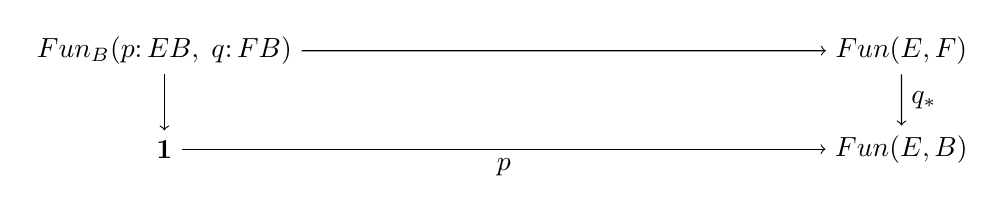
\begin{tikzpicture}[xscale=1.8,yscale=1.25]
\node (TL) at (0,1)
  {$\Fun_B(p\colon E\twoheadrightarrow B,\;q\colon F\twoheadrightarrow B)$};
\node (TR) at (5.2,1) {$\Fun(E,F)$};
\node (BL) at (0,0) {$\mathbf{1}$};
\node (BR) at (5.2,0) {$\Fun(E,B)$};
\draw[->] (TL) -- (TR);
\draw[->] (TL) -- (BL);
\draw[->] (TR) -- (BR) node[midway,right]{$q_\ast$};
\draw[->] (BL) -- (BR) node[midway,below]{$p$};
\node at (0.42,0.62) {$\scriptstyle\lrcorner$};
\end{tikzpicture}
\end{center}
且当指定的\trIsofibration{}在上下文中清楚时，
  缩记为 $\Fun_B(E,F)$
\item \trIsofibration{}是 $B$ 之上\trIsofibration{}的交换三角形
\begin{center}
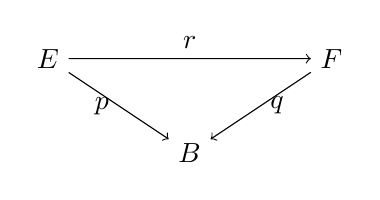
\begin{tikzpicture}[xscale=1.5,yscale=1.2]
\node (E) at (0,1) {$E$};
\node (F) at (2.4,1) {$F$};
\node (B) at (1.2,0) {$B$};
\draw[->] (E) -- (F) node[midway,above]{$r$};
\draw[->] (E) -- (B) node[pos=0.5,left]{$p$};
\draw[->] (F) -- (B) node[pos=0.5,right]{$q$};
\end{tikzpicture}
\end{center}
\item \trTerminal{}是 $\mathrm{id}\colon B\twoheadrightarrow B$，
  而积由沿对角的\trPullback{}定义
\begin{center}
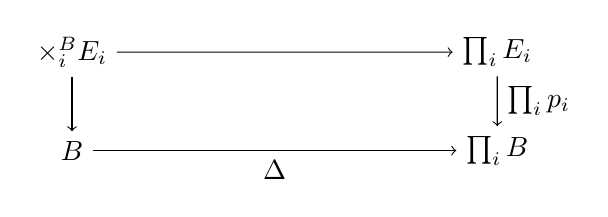
\begin{tikzpicture}[xscale=1.8,yscale=1.25]
\node (TL) at (0,1) {$\times_i^B E_i$};
\node (TR) at (3,1) {$\prod_i E_i$};
\node (BL) at (0,0) {$B$};
\node (BR) at (3,0) {$\prod_i B$};
\draw[->] (TL) -- (TR);
\draw[->] (TL) -- (BL);
\draw[->] (TR) -- (BR) node[midway,right]{$\prod_i p_i$};
\draw[->] (BL) -- (BR) node[midway,below]{$\Delta$};
\node at (0.42,0.62) {$\scriptstyle\lrcorner$};
\end{tikzpicture}
\end{center}
\item \trPullback{}与\trIsofibration{}之塔的\trLimit{}%
  由遗忘\trFunctor{} $\mathcal{K}_{/B}\to\mathcal{K}$ 造出
\item $p\colon E\twoheadrightarrow B$ 与 $U\in\sSet$
  的单纯\trCotensor{}由\trPullback{}构造
\begin{center}
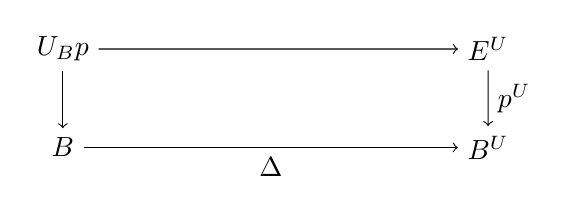
\begin{tikzpicture}[xscale=1.8,yscale=1.25]
\node (TL) at (0,1) {$U\pitchfork_B p$};
\node (TR) at (3,1) {$E^U$};
\node (BL) at (0,0) {$B$};
\node (BR) at (3,0) {$B^U$};
\draw[->] (TL) -- (TR);
\draw[->] (TL) -- (BL);
\draw[->] (TR) -- (BR) node[midway,right]{$p^U$};
\draw[->] (BL) -- (BR) node[midway,below]{$\Delta$};
\node at (0.42,0.62) {$\scriptstyle\lrcorner$};
\end{tikzpicture}
\end{center}
\item 并且其中 $B$ 之上的映射
\begin{center}
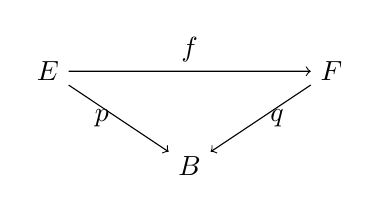
\begin{tikzpicture}[xscale=1.5,yscale=1.2]
\node (E) at (0,1) {$E$};
\node (F) at (2.4,1) {$F$};
\node (B) at (1.2,0) {$B$};
\draw[->] (E) -- (F) node[midway,above]{$f$};
\draw[->] (E) -- (B) node[pos=0.5,left]{$p$};
\draw[->] (F) -- (B) node[pos=0.5,right]{$q$};
\end{tikzpicture}
\end{center}
是\trInfinityCosmos{} $\mathcal{K}_{/B}$ 中的\trEquivalence{}，
  当且仅当 $f$ 是 $\mathcal{K}$ 中的\trEquivalence{}。
\end{enumerate}
\end{proposition}
\begin{proof}
\trFunctorSpace{}是\trQuasiCategory{}，
因为 \cref{def:infinity-cosmos}(ii) 断言：
对 $\mathcal{K}$ 中任何\trIsofibration{} $q\colon F\twoheadrightarrow B$，
映射 $q_\ast\colon\Fun(E,F)\twoheadrightarrow\Fun(E,B)$
是\trQuasiCategory{}的\trIsofibration{}。
该公理的其他部分蕴含：
每个\trLimit{}构造——如在 (iv) 与 (vi) 中构造的积与\trCotensor——
都定义 $B$ 之上的\trIsofibration{}。
$\mathcal{K}_{/B}$ 中\trIsofibration{}的诸封闭性质
从 $\mathcal{K}$ 中相应的封闭性质推出。
其中最复杂的是 $\mathcal{K}_{/B}$ 中\trIsofibration{}的
Leibniz \trCotensor{}稳定性，
它从 $\mathcal{K}$ 中相应的性质推出：
因为对\trSimplicialSet{}的\trMonomorphism $i\colon X\hookrightarrow Y$
与如上面 (iii) 中 $B$ 之上的\trIsofibration{} $r$，
映射 $i\widehat{\pitchfork}_B r$
由沿 $\Delta\colon B\to B^Y$ \trPullback $i\widehat{\pitchfork} r$ 而构造。

上述构造在一个单纯富集切片\trCategory{}中
定义单纯富集\trLimit{}这一事实，
是富集范畴论的标准结果。

只剩下验证\trIsofibration{}的\trInfinityCosmos{}中的%
\trEquivalence{}由遗忘\trFunctor{} $\mathcal{K}_{/B}\to\mathcal{K}$ 造出。
先设 (vii) 中所示的映射 $f$ 定义 $\mathcal{K}$ 中的\trEquivalence{}。
那么对任何\trIsofibration{} $s\colon A\twoheadrightarrow B$，
$\mathcal{K}_{/B}$ 中\trFunctorSpace{}上诱导的映射由\trPullback{}定义
\begin{equation*}
\begin{tikzpicture}[xscale=1.75,yscale=1.3]
\node (TL) at (0,2) {$\Fun_B(A,E)$};
\node (TR) at (4,2) {$\Fun(A,E)$};
\node (ML) at (1.7,1) {$\Fun_B(A,F)$};
\node (MR) at (5.6,1) {$\Fun(A,F)$};
\node (BL) at (0,0) {$\mathbf{1}$};
\node (BR) at (4,0) {$\Fun(A,B)$};
\draw[->] (TL) -- (TR) node[midway,above]{$f_\ast$};
\draw[->] (TL) -- (BL);
\draw[dashed,->] (TL) -- (ML) node[pos=0.5,above,sloped]{$\overset{\simeq}{f_\ast}$};
\draw[->] (ML) -- (MR) node[midway,above]{$p_\ast$};
\draw[->] (ML) -- (BL);
\draw[->] (TR) -- (MR) node[pos=0.45,above,sloped]{$\overset{\simeq}{f_\ast}$};
\draw[->] (TR) -- (BR) node[midway,right]{$p_\ast$};
\draw[->] (MR) -- (BR) node[pos=0.45,right]{$q_\ast$};
\draw[->] (BL) -- (BR) node[midway,below]{$s$};
\node at (0.42,1.62) {$\scriptstyle\lrcorner$};
\node at (2.12,0.62) {$\scriptstyle\lrcorner$};
\end{tikzpicture}
\end{equation*}
由于 $f$ 是 $\mathcal{K}$ 中的\trEquivalence{}，
映射 $f_\ast\colon\Fun(A,E)\to\Fun(A,F)$ 是\trEquivalence{}，
于是在 $s$ 之上的纤维上诱导的映射也是\trEquivalence{}。%
\footnote{\trIsofibration{}之间的\trEquivalence{}在\trPullback{}下的稳定性，
既可以作为\cref{lem:trivial-fibration-stability}与 \cref{lem:brown-factorization}的推论、
用单纯\trHomotopy{}论的标准技术来证明（见引理 C.1.11），
也可以按 2-\trCategory{}的方式论证（见命题 3.3.4）。}

对于逆蕴涵，我们求助于\cref{lem:equiv-homotopy-equivalences}。
若 $f\colon E\to F$ 是 $\mathcal{K}_{/B}$ 中的\trEquivalence{}，
则它在 $\mathcal{K}_{/B}$ 中容许\trHomotopy{}逆。
逆\trEquivalence{} $g\colon F\to E$ 也定义 $\mathcal{K}$ 中的逆\trEquivalence{}，
而 $\mathcal{K}$ 中所需的单纯\trHomotopy
\begin{equation*}
E\xrightarrow{\ \alpha\ }\mathbb{I}\pitchfork_B p\longrightarrow E^{\mathbb{I}}
\qquad\qquad
F\xrightarrow{\ \beta\ }\mathbb{I}\pitchfork_B q\longrightarrow F^{\mathbb{I}}
\end{equation*}
通过沿定义 $\mathcal{K}_{/B}$ 中\trCotensor{}的\trPullback{}之顶边作复合而定义。
\end{proof}

如\cref{dig:source-cosmoi-nature}中所提到的，
我们遇到的许多「野外」\trInfinityCosmos{}%
满足一条附加公理。
然而注意，这条公理不被\cref{prop:sliced-cosmoi}的切片\trInfinityCosmos{}继承，
这是它未被纳入\cref{def:infinity-cosmos}的原因之一。

\begin{definition}[\trCartesianClosed\trInfinityCosmos]\label{def:cartesian-closed-cosmoi}
一个\trInfinityCosmos{} $\mathcal{K}$ 是\textbf{\trCartesianClosed}
（cartesian closed），
如果积双\trFunctor{} $-\times-\colon\mathcal{K}\times\mathcal{K}\to\mathcal{K}$
扩充为一个单纯富集的双变量\trAdjunction
\begin{equation*}
\Fun(A\times B,C)\cong\Fun(A,C^B)\cong\Fun(B,C^A)
\end{equation*}
其中右\trAdjunction{} $(-)^A\colon\mathcal{K}\to\mathcal{K}$
对一切 $A\in\mathcal{K}$ 保持\trIsofibration{}。
\end{definition}
例如，\trQuasiCategory{}的\trInfinityCosmos{}是\trCartesianClosed{}，
其指数被定义为单纯\trCotensor{}的（特例）。
这正是我们对\trCotensor{}与指数使用同一记号的原因之一。
\footnote{这一方便的记号混用的其他优点
在 2.3 节与命题 10.3.5 中讨论。}

注意此时\trFunctorSpace{}与指数相重合。
\trCategory{}与\trKanComplex{}的笛卡尔封闭\trInfinityCosmos{}也是如此。
一般地，从 $A$ 到 $B$ 的\trFunctorSpace
是指数 $B^A$ 的「底\trQuasiCategory」——只要后者存在（见注 1.3.11）。

\begin{example}[$(\infty,1)$-\trCategory{}的\trInfinityCosmos{}；附录 E.2]\label{exa:cosmoi-models}
下列 $(\infty,1)$-\trCategory{}的模型定义\trCartesianClosed\trInfinityCosmos{}：
\begin{enumerate}[label=(\roman*)]
  \item Rezk 的\textbf{\trCompleteSegalSpaces}（complete Segal spaces）
  定义一个\trInfinityCosmos{} $\CSS$ 的对象，
  其中\trIsofibration{}、\trEquivalence{}与\trTrivialFibration
  是文献 \cite{bib100} 的\trModelStructure{}的相应类。%
  \footnote{警告：\trCompleteSegalSpaces{}的\trModelCategory
  在两个不同的「方向」上富集于\trSimplicialSet——
  一种富集使两个\trCompleteSegalSpaces{}之间的映射\trSimplicialSet
  成为\trKanComplex{}，探测「空间的」结构；
  另一种富集使映射\trSimplicialSet{}成为\trQuasiCategory{}，
  探测「\trCategory{}的」结构 \cite{bib64}。
  我们要的是后一种富集。}
\item 由 Dwyer、Kan 与 Smith \cite{bib38} 定义、
  并由 Hirschowitz 与 Simpson \cite{bib56} 发展的
  \textbf{\trSegalCategories}（Segal categories）
  定义一个\trInfinityCosmos{} $\mathcal{S}egal$ 的对象，
  其中\trIsofibration{}、\trEquivalence{}与\trTrivialFibration
  是文献 \cite{bib13,bib90} 的\trModelStructure{}的相应类。%
  \footnote{这里我们把术语「\trSegalCategories{}」保留给
  那些带有离散对象集、Reedy \trFibration{}且满足 Segal 条件的单纯对象。
  传统定义不包含 Reedy \trFibration{}条件，
  因为由\trKanComplex\trEnrichedCategory{}的\trNerve{}定义的单纯对象不满足它。
  由于\trKanComplex\trEnrichedCategory
  不在我们偏好的 $(\infty,1)$-\trCategory{}模型之列，
  这一点并不困扰我们。}
\item 文献 \cite{bib129} 的\textbf{\trOneComplicialSets}（1-complicial sets），
  \trEquivalence{}地，文献 \cite{bib78} 的「自然带标记\trQuasiCategory」，
  定义一个\trInfinityCosmos{} $1\text{-}\mathcal{C}omp$ 的对象，
  其中\trIsofibration{}、\trEquivalence{}与\trTrivialFibration
  是这两个来源中任一者的\trModelStructure{}的相应类。
\end{enumerate}
\end{example}

在附录 E.3 中，我们将证明
$(\infty,n)$-\trCategory{}乃至 $(\infty,\infty)$-\trCategory{}的某些模型
定义\trInfinityCosmos{}：
$n$-\trQuasiCategory{}、$\Theta_n$-空间、
迭代\trCompleteSegalSpaces{}以及 $n$-复状单纯集。

\begin{definition}[\trCodualInfinityCosmos]\label{def:co-dual-cosmoi}
存在一个对象上恒等的对合\trFunctor{}
$(-)^\circ\colon\boldsymbol{\Delta}\to\boldsymbol{\Delta}$，
它反转每个序数 $[n]\in\boldsymbol{\Delta}$ 中元素的顺序。
在 1.1.1 的记号下，\trFunctor $(-)^\circ$
把面映射 $\delta^i\colon[n-1]\rightarrowtail[n]$
送到面映射 $\delta^{n-i}\colon[n-1]\rightarrowtail[n]$，
并把退化映射 $\sigma^i\colon[n+1]\twoheadrightarrow[n]$
送到退化映射 $\sigma^{n-i}\colon[n+1]\twoheadrightarrow[n]$。
与这一对合自\trIsomorphism{}作\trPreComposition{}诱导一个对合
$(-)^{op}\colon\sSet\to\sSet$，
它把\trSimplicialSet $X$ 送到其\textbf{\trOppositeSimplicialSet}
（opposite simplicial set）$X^{op}$，
每个单纯形中顶点的定向被反转。
这一构造保持所有\trCone{}形\trLimit{}与\trColimit{}，
并在指数上诱导\trIsomorphism
$(Y^X)^{op}\cong(Y^{op})^{X^{op}}$。
\end{definition}

对任何\trInfinityCosmos{} $\mathcal{K}$，
存在一个\textbf{\trDualInfinityCosmos}
（dual ∞-cosmos）$\mathcal{K}^{co}$：
对象与 $\mathcal{K}$ 相同，但\trFunctorSpace{}定义为 %
\begin{equation*}
\Fun_{\mathcal{K}^{co}}(A,B):=\Fun_{\mathcal{K}}(A,B)^{op}.
\end{equation*}
$\mathcal{K}^{co}$ 中的\trIsofibration{}、\trEquivalence{}%
与\trTrivialFibration
与 $\mathcal{K}$ 中的相重合。

$\mathcal{K}^{co}$ 中的\trCone{}形\trLimit{}与 $\mathcal{K}$ 中的相重合，
而 $A\in\mathcal{K}$ 与 $U\in\sSet$ 的\trCotensor %
则定义为 $A^{U^{op}}$。

这一记号的一个 2-范畴论辩护见练习 1.4.ii。

\begin{definition}[离散\trInfinityCategory]\label{def:discrete-infinity-categories}
\trInfinityCosmos{} $\mathcal{K}$ 中的\trInfinityCategory{} $E$
是\textbf{\trDiscrete}（discrete），
如果对一切 $X\in\mathcal{K}$，
\trFunctorSpace $\Fun(X,E)$ 是\trKanComplex{}。
\end{definition}
在\trQuasiCategory{}的\trInfinityCosmos{}中，
离散\trInfinityCategory{}恰是\trKanComplex{}。
类似地，在\cref{exa:cosmoi-models}的那些\trInfinityCosmos{}中——
其\trInfinityCategory{}是某种模型下的 $(\infty,1)$-\trCategory——
离散\trInfinityCategory{}是\trInfinityGroupoid{}。
对下文重要的是，
离散\trInfinityCategory{}可以在\trInfinityCosmos{}之内
如下「内在地」刻画：

\begin{lemma}\label{lem:discrete-trivial-fibration}
\trInfinityCategory{} $E$ 是\trDiscrete{}，当且仅当
$E^{\mathbb{I}}\rvTfibArrow E^{\mathbf{2}}$ 是\trTrivialFibration{}。
\end{lemma}
\begin{proof}
由\cref{def:equivalence-trivial-fibration}，
\trIsofibration $E^{\mathbb{I}}\twoheadrightarrow E^{\mathbf{2}}$
是\trTrivialFibration{}，当且仅当对一切\trInfinityCategory{} $X$，
\trFunctorSpace{}上诱导的映射 %
\begin{equation*}
\begin{array}{ccc}
\Fun(X,E^{\mathbb{I}}) & \longrightarrow & \Fun(X,E^{\mathbf{2}})\\[0.4ex]
{\scriptstyle\cong}\downarrow & & \downarrow{\scriptstyle\cong}\\[0.4ex]
\Fun(X,E)^{\mathbb{I}} & \longrightarrow & \Fun(X,E)^{\mathbf{2}}
\end{array}
\end{equation*}
是\trQuasiCategory{}的\trTrivialFibration{}。
经由单纯\trCotensor{}的泛性质，
引理 1.1.30 告诉我们：
该映射是\trTrivialFibration{}，当且仅当 $\Fun(X,E)$ 是\trKanComplex{}。
\end{proof}
读者可以验证：
任何\trInfinityCosmos{}中的离散\trInfinityCategory{}%
装配成一个\trInfinityCosmos{} $\mathcal{K}^{\simeq}$。
证明见命题 6.1.6，
那里发展了从给定者产生新的\trInfinityCosmos{}的一般技术。

\subsection*{练习}

\begin{exercise}\label{ex:simplicial-versus-enriched}
在下列二\trCategory{}之间定义\trEquivalence{}：
\begin{enumerate}[label=(\roman*)]
  \item \trSimplicialCategory{}，如 \eqref{eq:simplicial-category-diagram} 中者，与
\item 富集于\trSimplicialSet{}的\trCategory{}。
\end{enumerate}
\end{exercise}

\begin{exercise}\label{ex:conical-products-qcat}
详细展开\cref{prop:cosmos-quasi-categories}的证明：
证明\trSimpliciallyEnrichedCategory $\QCat$
容许满足\cref{dig:simplicially-enriched-limits}之泛性质的\trCone{}形积。即：
\begin{enumerate}[label=(\roman*)]
\item 定义一对\trQuasiCategory $A$ 与 $B$ 的笛卡尔积 $A\times B$
  及投影映射 $\pi_A\colon A\times B\to A$
  与 $\pi_B\colon A\times B\to B$，
  并证明这组数据满足通常的（非富集的）泛性质。
\item 给定另一个\trQuasiCategory $X$，
  用 (i) 与\trYonedaLemma{}证明投影映射诱导\trQuasiCategory{}的\trIsomorphism
  \begin{equation*}
  (A\times B)^X\xrightarrow{\ \simeq\ }A^X\times B^X.
  \end{equation*}
\item 解释这与\cref{dig:simplicially-enriched-limits}的泛性质有何关系。
\item 把 (i) 的通常 1-范畴论泛性质
  表述为 (ii) 之泛性质的「$0$ 维面向」。
\end{enumerate}
\end{exercise}

\begin{exercise}\label{ex:path-object}
证明\trInfinityCosmos{}中的任何对象都有\textbf{\trPathObject}
（path object）
\begin{center}
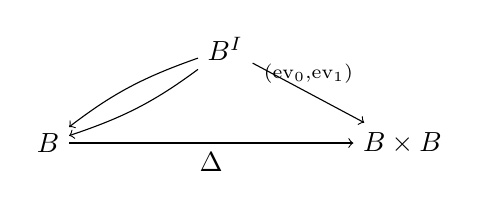
\begin{tikzpicture}[xscale=1.5,yscale=1.2]
\node (Bi) at (1.5,1) {$B^{\mathbb{I}}$};
\node (B) at (0,0) {$B$};
\node (BB) at (3,0) {$B\times B$};
\draw[->] (Bi) to[bend right=10] (B);
\draw[->] (Bi) to[bend left=10] (B);
\draw[->] (Bi) -- (BB) node[midway,above]{$\scriptstyle(\mathrm{ev}_0,\mathrm{ev}_1)$};
\draw[->] (B) -- (BB) node[midway,below]{$\Delta$};
\end{tikzpicture}
\end{center}
它由与\trFreeLivingIsomorphism{}作\trCotensor{}而构造。
\end{exercise}

\begin{exercise}\label{ex:dual-cartesian-closed}
证明：若 $\mathcal{K}$ 是\trCartesianClosed\trInfinityCosmos{}，
则 $\mathcal{K}^{co}$ 亦然。
\end{exercise}

\begin{exercise}[6.1.6]\label{ex:discrete-cosmos}
用\cref{prop:cosmos-kan-complexes}证明：
任何\trInfinityCosmos{}中的离散\trInfinityCategory{}%
定义一个\trInfinityCosmos{}，
其\trFunctorSpace{}皆为\trKanComplex{}。
\end{exercise}
   %
\providecommand{\Fun}{\operatorname{Fun}}
\providecommand{\QCat}{\mathcal{Q}\mathcal{C}at}
\providecommand{\CSS}{\mathcal{CSS}}
\providecommand{\Cat}{\mathcal{C}at}
\providecommand{\rvTfibArrow}{\mathrel{\stackrel{\sim}{\twoheadrightarrow}}}
\providecommand{\rvEqArrow}{\mathrel{\stackrel{\sim}{\Rightarrow}}} %
\section{\trCosmologicalFunctor}\label{sec:cosmological-functors}

某些「右\trAdjunction{}型」的构造定义了\trInfinityCosmos{}之间的映射，
这些映射保持定义 1.2.1 中公理化的全部结构。%
这类构造定义\trInfinityCosmos{}之间的\emph{\trCosmologicalFunctor}
（cosmological functor）——这一简单的观察使许多证明变得精简。

\begin{definition}[\trCosmologicalFunctor]\label{def:cosmological-functor}
\textbf{\trCosmologicalFunctor}是一个\trInfinityCosmos{}之间的
\textbf{\trSimplicialFunctor}（simplicial functor；见定义 A.2.6），%
它保持指定的\trIsofibration{}与全部宇宙论\trLimit{}。
\end{definition}

一般地，\trCosmologicalFunctor{}保持任何能在\trInfinityCosmos{}\emph{内部}刻画的
∞-范畴论概念——例如，作为配有附加结构的映射——与之相对的是
\emph{外部}刻画的概念——例如，由一条涉及全称量词或存在量词的
陈述所作的刻画。例如，\trInfinityCosmos{}中的\trEquivalence{}%
在定义 1.2.2 中是外部刻画的，%
这可能让人怀疑，一个非满射的\trCosmologicalFunctor{}或许无法保持它们。
然而，引理 1.2.15 把\trEquivalence{}刻画为\trInfinityCosmos{}内部
定义的诸结构之存在性，%
于是作为结论：

\begin{lemma}\label{lem:cosmological-preserves-equivalences}
任何\trCosmologicalFunctor{}还保持\trEquivalence{}与\trTrivialFibration{}。
\end{lemma}
\begin{proof}
由引理 1.2.15，%
\trInfinityCosmos{}中的\trEquivalence{}与「\trHomotopy\trEquivalence」重合，
后者由与\trFreeLivingIsomorphism{}作\trCotensor{}来定义。由于\trCosmologicalFunctor{}保持单纯\trCotensor{}，
它保持 (1.2.16) 中所示的数据，%
从而把\trEquivalence{}送到\trEquivalence{}。\trTrivialFibration{}的保持随之而得。
\end{proof}

\begin{remark}\label{rem:cosmological-discrete-categories}
类似地，单从定义 1.2.26 出发论证，%
并不清楚\trCosmologicalFunctor{}是否保持离散\trInfinityCategory{}；
但利用引理 1.2.27 的内部刻画——%
\trInfinityCategory{} $A$ 是\trDiscrete{}，当且仅当
$A^{\mathbb{I}}\rvTfibArrow A^{\mathbf{2}}$ 是\trTrivialFibration——
这一点便由\trCosmologicalFunctor{}保持单纯\trCotensor{}与\trTrivialFibration{}的事实得出。
\end{remark}

我们现在证明\trCosmologicalFunctor{}是大量存在的：

\begin{proposition}\label{prop:cosmological-functor-constructions}
下列构造对任何\trInfinityCosmos{} $\mathcal{K}$ 都定义\trCosmologicalFunctor{}：
\begin{enumerate}[label=(\roman*)]
\item \trFunctorSpace $\Fun(X,-)\colon\mathcal{K}\to\QCat$，
  对任何\trInfinityCategory{} $X$。
\item \textbf{底\trQuasiCategory}（underlying quasi-category）\trFunctor
  \[
  (-)_0\coloneqq\Fun(1,-)\colon\mathcal{K}\to\QCat,
  \]
  即把 (i) 特化到\trTerminal{}\trInfinityCategory{} $1$。
\item 单纯\trCotensor $(-)^U\colon\mathcal{K}\to\mathcal{K}$，
  对任何\trSimplicialSet $U$。
\item 指数 $(-)^A\colon\mathcal{K}\to\mathcal{K}$，对\trCartesianClosed
  \trInfinityCosmos{} $\mathcal{K}$ 中任何\trInfinityCategory{} $A$。
\item 沿\trInfinityCosmos{} $\mathcal{K}$ 中任何\trFunctor{}
  $f\colon A\to B$ 取\trIsofibration{}的\trPullback
  $f^\ast\colon\mathcal{K}_{/B}\to\mathcal{K}_{/A}$。
\item 而且，对任何\trCosmologicalFunctor $F\colon\mathcal{K}\to\mathcal{L}$
  与任何\trInfinityCategory{} $A\in\mathcal{K}$，
  切片上诱导的映射 $F\colon\mathcal{K}_{/A}\to\mathcal{L}_{/FA}$
  定义一个\trCosmologicalFunctor{}。
\end{enumerate}
\end{proposition}

\begin{proof}
这前四条陈述几乎是立即可得的：\trIsofibration{}的保持在其中每个情形
都被显式断言为一条假设，而\trLimit{}的保持则来自熟悉的论证。

对 (v)，\trInfinityCosmos{} $\mathcal{K}$ 中的\trPullback{}是一个单纯富集的%
\trLimit{}构造；它的一个后果是%
$f^\ast\colon\mathcal{K}_{/B}\to\mathcal{K}_{/A}$
定义一个\trSimplicialFunctor{}。\trFunctor{} $f^\ast$ 在 $\mathcal{K}_{/B}$ 中
0-箭头 $g$ 上的作用同样由一个\trPullback{}方块定义：由于所示图表的前、后
两个方块都是\trPullback{}，顶上的方块亦然
\begin{equation*}
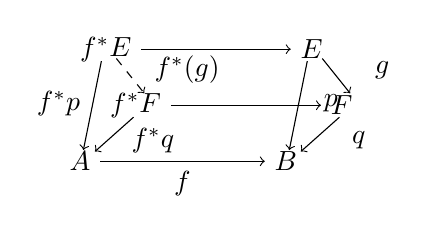
\begin{tikzpicture}[x=1.55em,y=1.35em]
  \node (fsE) at (0.6,3)   {$f^\ast E$};
  \node (E)   at (5.4,3)   {$E$};
  \node (fsF) at (1.3,1.5) {$f^\ast F$};
  \node (F)   at (6.1,1.5) {$F$};
  \node (A)   at (0,0)     {$A$};
  \node (B)   at (4.8,0)   {$B$};
  \draw[->] (fsE) -- (E);
  \draw[->] (fsF) -- (F);
  \draw[->] (A) -- (B) node[midway,below]{$f$};
  \draw[->] (0.5,2.68) -- (0.08,0.3);
  \node at (-0.5,1.55) {$f^\ast p$};
  \draw[->,dashed] (0.85,2.75) -- (1.5,1.82);
  \node at (2.5,2.45) {$f^{\ast}(g)$};
  \draw[->] (1.25,1.18) -- (0.35,0.26);
  \node at (1.7,0.55) {$f^\ast q$};
  \draw[->] (5.3,2.68) -- (4.88,0.3);
  \node at (5.85,1.55) {$p$};
  \draw[->] (5.65,2.75) -- (6.3,1.82);
  \node at (7.05,2.45) {$g$};
  \draw[->] (6.05,1.18) -- (5.15,0.26);
  \node at (6.5,0.55) {$q$};
  \node at (1.05,2.6) {$\scriptstyle\lrcorner$};
  \node at (1.75,1.32) {$\scriptstyle\lrcorner$};
\end{tikzpicture}
\end{equation*}
由于\trIsofibration{}在\trPullback{}下稳定，可知
$f^\ast\colon\mathcal{K}_{/B}\to\mathcal{K}_{/A}$
保持\trIsofibration{}。剩下要证这个\trFunctor{}保持
命题 1.2.22 中构造的那些单纯\trLimit{}，%
而这根本上是\trLimit{}构造之交换性的一个后果。
每种情形都可以显式验证。我们以构造交换立方体为例，
演示单纯\trCotensor{}情形的这一计算：
\begin{equation*}
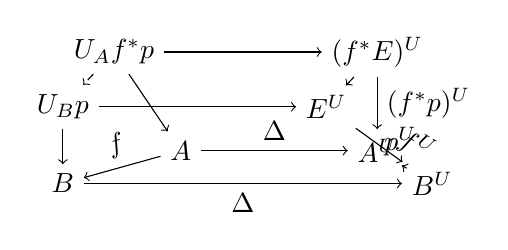
\begin{tikzpicture}[x=1.42em,y=1.32em]
  \node (tfl) at (1.3,3.6) {$U\pitchfork_A f^\ast p$};
  \node (tfr) at (8.0,3.6) {$(f^\ast E)^U$};
  \node (tbl) at (0,2.1)   {$U\pitchfork_B p$};
  \node (tbr) at (6.7,2.1) {$E^U$};
  \node (bfl) at (3.0,0.9) {$A$};
  \node (bfr) at (8.0,0.9) {$A^U$};
  \node (bbl) at (0,0)     {$B$};
  \node (bbr) at (9.4,0)   {$B^U$};
  \draw[->] (tfl) -- (tfr);
  \draw[->,dashed] (tfl) -- (tbl);
  \draw[->] (tbl) -- (tbr);
  \draw[->] (tfr) -- (tbr);
  \draw[->] (tfl) -- (bfl);
  \draw[->] (tbl) -- (bbl);
  \draw[->] (tfr) -- (bfr) node[midway,right]{$(f^\ast p)^U$};
  \draw[->] (tbr) -- (bbr) node[pos=0.4,right]{$p^U$};
  \draw[->] (bfl) -- (bfr) node[midway,above]{$\Delta$};
  \draw[->] (bbl) -- (bbr) node[midway,below]{$\Delta$};
  \draw[->] (bfl) -- (bbl) node[pos=0.5,above,sloped]{$f$};
  \draw[->] (bfr) -- (bbr) node[pos=0.5,above,sloped]{$f^U$};
  \node at (2.5,3.32) {$\scriptstyle\lrcorner$};
  \node at (0.42,1.82) {$\scriptstyle\lrcorner$};
  \node at (7.7,3.3) {$\scriptstyle\lrcorner$};
\end{tikzpicture}
\end{equation*}
由于前、后、右三个面都是\trPullback{}，左面亦然。
最后一条陈述 (vi) 留作\cref{ex:slice-induced-cosmological}。
\end{proof}

\begin{example}\label{exa:cat-kan-cosmological-embeddings}
由命题 1.2.11 与 1.2.12，%
满子\trCategory{}包含 $\Cat\hookrightarrow\QCat$ 与
$\mathcal{K}an\hookrightarrow\QCat$ 都定义\trCosmologicalFunctor
（另见引理 6.1.4）。%
这些\trCosmologicalEmbedding{}阐明了如下直觉：1-\trCategory{}或\trInfinityGroupoid{}的形式范畴论
可以作为 $(\infty,1)$-\trCategory{}的形式范畴论之特例而恢复。
\end{example}

\trCosmologicalFunctor{}的非例同样富有教益： %

\begin{nonexample}\label{exa:forgetful-not-cosmological}
遗忘\trFunctor{} $\mathcal{K}_{/B}\to\mathcal{K}$ 是单纯的
且保持\trIsofibration{}，却并\emph{不}定义\trCosmologicalFunctor{}：
它不保持\trCotensor{}与积。然而，
由\cref{prop:cosmological-functor-constructions}(v)，
其右\trAdjunction{} $-\times B\colon\mathcal{K}\to\mathcal{K}_{/B}$
确实定义一个\trCosmologicalFunctor{}。
\end{nonexample}

\begin{nonexample}\label{exa:core-not-cosmological}
\trCosmologicalEmbedding $\mathcal{K}an\hookrightarrow\QCat$ 有一个右\trAdjunction{}
$(-)^{\simeq}\colon\QCat\to\mathcal{K}an$，它把每个\trQuasiCategory{}%
送到其「\trInfinityGroupoidCore」——即\trMaximalSubKanComplex{}，%
由那些所有边皆为\trIsomorphism{}的 $n$-单纯形组成的单纯子集。
这一核\trFunctor{}保持\trIsofibration{}与 1-范畴论的\trLimit{}，
却不是\trCosmologicalFunctor{}，因为它不是单纯富集的：
任何定义域为\trKanComplex{}而陪域为\trQuasiCategory{}的\trFunctor{}
$K\to Q$ 都经由一个唯一的映射 $K\to Q^{\simeq}$
分解而穿过包含 $Q^{\simeq}\hookrightarrow Q$，
但一般地 $\Fun(K,Q)\ncong\Fun(K,Q^{\simeq})$，
因为\trNaturalTransformation $K\times\Delta[1]\to Q$
只有在其各分量都可逆时才穿过 $Q^{\simeq}\hookrightarrow Q$ 分解
（不过见引理 12.1.12）。%
\end{nonexample}

某些\trCosmologicalFunctor{}的表现格外良好：

\begin{definition}[宇宙论\trBiequivalence{}]\label{def:cosmological-biequivalence}
一个\trCosmologicalFunctor{}定义一个\textbf{宇宙论\trBiequivalence}
（cosmological biequivalence）
$F\colon\mathcal{K}\Rightarrow\mathcal{L}$，如果它还
\begin{enumerate}[label=(\roman*)]
\item 是\textbf{对象在\trEquivalence{}意义下本质满射的}
  （essentially surjective on objects up to equivalence）：
  对一切 $C\in\mathcal{L}$，存在 $A\in\mathcal{K}$
  使得 $FA\simeq C$，并且
\item 定义一个\textbf{局部\trEquivalence}（local equivalence）：
  对一切 $A,B\in\mathcal{K}$，$F$ 在\trFunctorSpace{}上的作用定义%
  \trQuasiCategory{}的\trEquivalence
  \[
  \Fun(A,B)\xrightarrow{\ \sim\ }\Fun(FA,FB).
  \]
\end{enumerate}
\end{definition}

宇宙论\trBiequivalence{}在第 10 章中得到更系统的研究，
在那里我们把它们设想为「\trChangeOfModel{}」\trFunctor{}。
对我们在第 11 章中证明 $(\infty,1)$-范畴论的
「\trModelIndependence{}」而言至关重要的是，
在 $(\infty,1)$-\trCategory{}的诸\trInfinityCosmos{}之间
存在着多种多样的宇宙论\trBiequivalence{}：

\begin{example}[附录 E.2]\label{exa:biequivalences-models}
\begin{enumerate}[label=(\roman*)]
\item 定义在\trCompleteSegalSpaces{}、\trSegalCategories{}与\trOneComplicialSets{}的
  诸\trInfinityCosmos{}上的底\trQuasiCategory\trFunctor
  \[
  \CSS\xrightarrow{\;(-)_0\;}\QCat\qquad
  \mathcal{S}egal\xrightarrow{\;(-)_0\;}\QCat\qquad
  1\text{-}\mathcal{C}omp\xrightarrow{\;(-)_0\;}\QCat
  \]
  都是\trBiequivalence{}。前两种情形由「在第 0 行取值」定义，
  最后一种情形则由「遗忘标记」定义。
\item 还有由 Joyal 与 Tierney \cite{bib64} 定义的宇宙论\trBiequivalence{}
  $\mathrm{nerve}\colon\QCat\Rightarrow\CSS$
  与 $\mathrm{nerve}\colon\QCat\Rightarrow\mathcal{S}egal$。
\item 由 Bergner \cite{bib14} 定义、把\trCompleteSegalSpaces
  「离散化」的\trFunctor{}
  $\mathrm{disc}\colon\CSS\Rightarrow\mathcal{S}egal$
  也定义一个宇宙论\trBiequivalence{}。
\item 另一个宇宙论\trBiequivalence{}
  $(-)^{\flat}\colon\QCat\Rightarrow 1\text{-}\mathcal{C}omp$
  给每个\trQuasiCategory{}配上其「自然标记」。
\end{enumerate}
\end{example}

用命题 10.2.1 所证成的术语来说： %

\begin{definition}\label{def:cosmos-of-infinity-one-categories}
一个\trInfinityCosmos{} $\mathcal{K}$ 是
\textbf{$(\infty,1)$-\trCategory{}的\trInfinityCosmos}
（$\infty$-cosmos of ($\infty$,1)-categories），
当且仅当底\trQuasiCategory\trFunctor $(-)_0\colon\mathcal{K}\to\QCat$
是一个宇宙论\trBiequivalence{}。
\end{definition}

\begin{remark}\label{rem:underlying-qcat-internal-homs}
底\trQuasiCategory\trFunctor $(-)_0\colon\mathcal{K}\to\QCat$
把笛卡尔封闭\trInfinityCosmos{} $\mathcal{K}$ 的\trInternalHom
送到相应的\trFunctorSpace{}：对 $\mathcal{K}$ 中任何\trInfinityCategory{}
$A$ 与 $B$，我们有
\[
(B^A)_0\coloneqq\Fun(1,B^A)\cong\Fun(A,B).
\]
\end{remark}
在\trInfinityCosmos{} $\mathcal{K}$ 与 $\QCat$
\trBiequivalence{}的情形，
我们在第 10 章与第 11 章中将会看到，
这不造成范畴论信息的本质损失。

宇宙论\trBiequivalence{}不仅保持\trEquivalence{}，还会反映并创造它们。

\begin{lemma}\label{lem:biequivalence-reflect-create}
设 $F\colon\mathcal{K}\Rightarrow\mathcal{L}$
是一个宇宙论\trBiequivalence{}。那么：
\begin{enumerate}[label=(\roman*)]
\item $\mathcal{K}$ 中\trInfinityCategory{}之间的\trFunctor{}
  $f\colon A\to B$ 是\trEquivalence{}，当且仅当
  $Ff\colon FA\rvEqArrow FB$ 是 $\mathcal{L}$ 中的\trEquivalence{}。
\item $\mathcal{K}$ 中的一对\trInfinityCategory{}是\trEquivalence{}的，
  当且仅当它们在 $\mathcal{L}$ 中的像是\trEquivalence{}的。
\end{enumerate}
\end{lemma}
\begin{proof}
\cref{lem:cosmological-preserves-equivalences} 蕴含：
\trCosmologicalFunctor{}保持\trEquivalence{}，因而也保持 $\mathcal{K}$ 中
一对\trInfinityCategory{}之间\trEquivalence{}的存在性。
为见\trEquivalence{}也被反映，设 $f\colon A\to B$
是 $\mathcal{K}$ 中一个\trFunctor{}，具有如下性质：
$Ff\colon FA\rvEqArrow FB$ 是 $\mathcal{L}$ 中的\trEquivalence{}。
现在对任何\trInfinityCategory{} $X$，
\trSimplicialFunctor{}性给出交换方块
\begin{equation*}
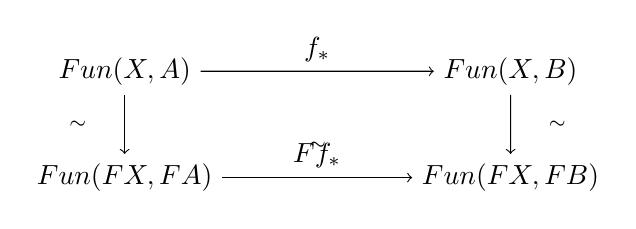
\begin{tikzpicture}[xscale=1.75,yscale=1.35]
\node (TL) at (0,1) {$\Fun(X,A)$};
\node (TR) at (2.8,1) {$\Fun(X,B)$};
\node (BL) at (0,0) {$\Fun(FX,FA)$};
\node (BR) at (2.8,0) {$\Fun(FX,FB)$};
\draw[->] (TL) -- (TR) node[midway,above]{$f_\ast$};
\draw[->] (TL) -- (BL);
\node at (-0.34,0.5) {$\scriptstyle\sim$};
\draw[->] (TR) -- (BR);
\node at (3.14,0.5) {$\scriptstyle\sim$};
\draw[->] (BL) -- (BR) node[midway,above]{$Ff_\ast$};
\node at (1.4,0.3) {$\scriptstyle\sim$};
\end{tikzpicture}
\end{equation*}

于是由\trTwoOfThreeProperty{}可得
$f_\ast\colon\Fun(X,A)\rvEqArrow\Fun(X,B)$ 是\trEquivalence{}，
这就证明了 $f$ 是 $\mathcal{K}$ 中的\trEquivalence{}。

为见\trEquivalence{}也会被创造，现在设 $A$ 与 $B$
是 $\mathcal{K}$ 中配有\trEquivalence{}的\trInfinityCategory
\begin{equation*}
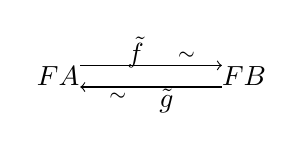
\begin{tikzpicture}[x=1.6em,y=1.3em]
  \node (FA) at (0,0) {$FA$};
  \node (FB) at (4.2,0) {$FB$};
  \draw[->] (0.5,0.3) -- (3.7,0.3);
  \node at (1.75,0.66) {$\tilde{f}$};
  \node at (2.9,0.56) {$\scriptstyle\sim$};
  \draw[->] (3.7,-0.3) -- (0.5,-0.3);
  \node at (2.45,-0.68) {$\tilde{g}$};
  \node at (1.35,-0.58) {$\scriptstyle\sim$};
\end{tikzpicture}
\end{equation*}
\begin{equation*}
\begin{tikzpicture}[xscale=1.35,yscale=1.05]
\node (lA) at (0,0) {$FA$};
\node (tA) at (2.2,1.3) {$FA$};
\node (Ai) at (2.2,0) {$FA^{\mathbb{I}}$};
\node (bA) at (2.2,-1.3) {$FA$};
\draw[double] (lA) -- (tA);
\draw[->] (Ai) -- (tA) node[midway,right]{$\mathrm{ev}_0$};
\draw[->] (lA) -- (Ai) node[midway,above]{$\alpha$};
\draw[->] (lA) -- (bA) node[midway,below]{$\tilde{g}\tilde{f}$};
\draw[->] (Ai) -- (bA) node[midway,right]{$\mathrm{ev}_1$};
\node (lB) at (7,0) {$FB$};
\node (tB) at (9.2,1.3) {$FB$};
\node (Bi) at (9.2,0) {$FB^{\mathbb{I}}$};
\node (bB) at (9.2,-1.3) {$FB$};
\draw[->] (lB) -- (tB) node[midway,above]{$\tilde{f}\tilde{g}$};
\draw[->] (Bi) -- (tB) node[midway,right]{$\mathrm{ev}_0$};
\draw[->] (lB) -- (Bi) node[midway,above]{$\beta$};
\draw[double] (lB) -- (bB);
\draw[->] (Bi) -- (bB) node[midway,right]{$\mathrm{ev}_1$};
\end{tikzpicture}
\end{equation*}
（在 $\mathcal{L}$ 中）。由于
$\Fun(A,B)\rvEqArrow\Fun(FA,FB)$ 与
$\Fun(B,A)\rvEqArrow\Fun(FB,FA)$ 是\trQuasiCategory{}的\trEquivalence{}，
由注 1.1.24，%
其诱导的\trHomotopyCategory\trFunctor{}
$\mathrm{h}(\Fun(A,B))\rvEqArrow\mathrm{h}(\Fun(FA,FB))$
与 $\mathrm{h}(\Fun(B,A))\rvEqArrow\mathrm{h}(\Fun(FB,FA))$
是\trCategory{}的\trEquivalence{}，从而特别地本质满射。
于是我们可以把 $\tilde{f}$ 与 $\tilde{g}$ 分别\trLifting{}为
$\mathrm{h}(\Fun(A,B))$ 与 $\mathrm{h}(\Fun(B,A))$
中的\trFunctor{} $f\colon A\to B$ 与 $g\colon B\to A$，
使得 $Ff\cong\tilde{f}$ 且 $Fg\cong\tilde{g}$。
\trQuasiCategory{}的交换方块
\begin{equation*}
\begin{tikzpicture}[xscale=2.0,yscale=1.4]
\node (TL) at (0,1) {$\Fun(B,A)\times\Fun(A,B)$};
\node (TR) at (4.4,1) {$\Fun(A,A)$};
\node (BL) at (0,0) {$\Fun(FB,FA)\times\Fun(FA,FB)$};
\node (BR) at (4.4,0) {$\Fun(FA,FA)$};
\draw[->] (TL) -- (TR) node[midway,above]{$\circ$};
\draw[->] (TL) -- (BL);
\node at (-0.55,0.5) {$\scriptstyle\sim$};
\draw[->] (TR) -- (BR);
\node at (4.95,0.5) {$\scriptstyle\sim$};
\draw[->] (BL) -- (BR) node[midway,above]{$\circ$};
\end{tikzpicture}
\end{equation*}
在其\trHomotopyCategory{}之间诱导一个交换方块。特别地，
把复合双\trFunctor{}用于\trIsomorphism $Ff\cong\tilde{f}$ 与 $Fg\cong\tilde{g}$，
我们看到在 $\mathrm{h}(\Fun(A,A))$ 中
\[
F(\mathrm{id}_A)=\mathrm{id}_{FA}
\cong\tilde{g}\circ\tilde{f}
\cong Fg\circ Ff=F(g\circ f)
\]
由 $\mathrm{h}(\Fun(A,A))\rvEqArrow\mathrm{h}(\Fun(FA,FA))$
的全忠实性，这一\trIsomorphism\trLifting{}为 $\mathrm{h}(\Fun(A,A))$
中的\trIsomorphism $\mathrm{id}_A\cong g\circ f$。
由推论 1.1.16，%
这一\trIsomorphism{}可以由一个\trHomotopyCoherentIsomorphism $\mathbb{I}\to\Fun(A,A)$
表示，后者内部化而定义所需的映射
$\alpha\colon A\to A^{\mathbb{I}}$。
从 $f\circ g$ 到 $\mathrm{id}_B$ 的\trHomotopyCoherentIsomorphism
$\beta\colon B\to B^{\mathbb{I}}$ 之构造与此类似。
\end{proof}

\cref{lem:biequivalence-reflect-create} 中\trEquivalence{}之创造的证明出人意料地精细：
它转入\trFunctorSpace{}的\trHomotopyCategory{}，以避免\trLifting{}并复合\trHomotopyCoherentIsomorphism{}；
循此路线的论证也是可能的，
留作\cref{ex:biequivalence-creation-sketch}由读者完成。
下一节将通过引入\trInfinityCosmos{}的\trHomotopyTwoCategory{}%
为刚才给出的论证提供语境。随后请读者在练习 1.4.vi 中
重温\trEquivalence{}的创造。%

\subsection*{练习}

\begin{exercise}\label{ex:slice-induced-cosmological}
证明：对任何\trCosmologicalFunctor $F\colon\mathcal{K}\to\mathcal{L}$
与任何 $A\in\mathcal{K}$，
切片上诱导的映射 $F\colon\mathcal{K}_{/A}\to\mathcal{L}_{/FA}$
定义一个\trCosmologicalFunctor{}。
\end{exercise}

\begin{exercise}\label{ex:biequivalence-creation-sketch}
概述一个证明：宇宙论\trBiequivalence{}创造\trInfinityCategory{}之间的%
\trEquivalence{}而无须转入\trHomotopyCategory——办法是把作为所设%
\trEquivalence{}数据之一部分给出的那些\trHomotopyCoherentIsomorphism%
\trLifting{}并复合起来。
\end{exercise}

\begin{exercise}\label{ex:biequivalence-cancellation}
设 $F\colon\mathcal{K}\to\mathcal{L}$、
$G\colon\mathcal{L}\to\mathcal{M}$
与 $H\colon\mathcal{M}\to\mathcal{N}$
都是\trCosmologicalFunctor{}，并设 $GF$ 与 $HG$ 是宇宙论\trBiequivalence{}。
证明：$F$、$G$、$H$ 与 $HGF$ 都是宇宙论\trBiequivalence{}。
\end{exercise}
   %
\providecommand{\Fun}{\operatorname{Fun}}
\providecommand{\Cat}{\mathcal{C}at}
\providecommand{\sSet}{s\mathcal{S}et}
\providecommand{\QCat}{\mathcal{Q}\mathcal{C}at}
\providecommand{\qcOne}{\mathbf{1}}  %
\providecommand{\qcTwo}{\mathbf{2}}  %
\providecommand{\qcInt}{\mathbb{I}}  %
\providecommand{\rvEqArrow}{\mathrel{\stackrel{\sim}{\Rightarrow}}} %
\providecommand{\rvTfibArrow}{\mathrel{\stackrel{\sim}{\twoheadrightarrow}}} %
\providecommand{\hcat}[1]{\hbar #1}  %
\providecommand{\rvCorner}[1]{\ulcorner #1\urcorner} %
\providecommand{\hTwoCell}[5]{\tikz[baseline=-0.8ex]{%
  \node (rvl) at (0,0) {$#1$};
  \node (rvr) at (2.9,0) {$#2$};
  \draw[->] (rvl) to[bend left=28] node[above]{$\scriptstyle #3$} (rvr);
  \draw[->] (rvl) to[bend right=28] node[below]{$\scriptstyle #5$} (rvr);
  \node at (1.45,0) {$\scriptstyle #4$};}}

\section{\trHomotopyTwoCategory}\label{sec:homotopy-2-category}

小 1-\trCategory{}作为对象构成一个由\trCategory{}、\trFunctor{}与\trNaturalTransformation{}组成的%
严格的\textbf{2-\trCategory}（2-category）\footnote{附录 B 介绍 2-\trCategory{}与 2-\trFunctor{}，
综述此处所需的 2-范畴论。简言之，与题外话 1.2.4 相平行地，%
2-\trCategory{}（见附录 B 中的\cref{def:two-category}）
可以同等地理解为：「二维」的\trCategory——有对象；1-\trCell{}，其边缘由一对对象给出；
以及 2-\trCell{}，其边缘由一对对象之间的一对平行 1-\trCell{}给出——连同由这份边缘数据
支配的、部分定义的复合操作；或者理解为富集于 $\Cat$ 之上的\trCategory{}。} $\Cat$。
许多基本的范畴论概念——即那些借助\trCategory{}、\trFunctor{}与\trNaturalTransformation{}%
定义的概念——都可以在 2-\trCategory $\Cat$ 内部定义。这暗示出一条自然的推广途径：
在一般的 2-\trCategory{}中重新解释这些同样的定义——用其对象代替小\trCategory{}，
用其\textbf{1-\trCell}（1-cell）代替\trFunctor{}，
用其\textbf{2-\trCell}（2-cell）代替\trNaturalTransformation{}。

在第 2 章中，我们将完全按照这一提纲，在任意取定的一个\trInfinityCosmos{}内部
发展\trInfinityCategory{}理论的相当大一部分：我们将在一座 2-\trCategory{}之中工作，
这座 2-\trCategory{}就是我们配属于任何\trInfinityCosmos{}的\emph{\trHomotopyTwoCategory}。
\trInfinityCosmos{}的\trHomotopyTwoCategory{}是整个\trInfinityCosmos{}的一个商：
把每个\trQuasiCategory{}性的\trFunctorSpace{}换成它的\trHomotopyCategory{}。令人惊讶的是，
这一颇具破坏性的取商操作竟保住了相当多的信息。事实上，
第一部分中\trInfinityCategory{}理论的几乎全部发展都发生于某个\trInfinityCosmos{}的%
\trHomotopyTwoCategory{}之中。话虽如此，我们还是要告诫读者切勿过度迷恋\trHomotopyTwoCategory{}：
与其说它是\trInfinityCategory{}理论的一个基础性概念，
不如说它是降低论证复杂度的一种技术性便利。

\trQuasiCategory{}之\trInfinityCosmos{}的\trHomotopyTwoCategory{}由 Joyal 在其关于\trQuasiCategory{}理论基础的
著作中率先引入\cite{bib63}。

\begin{definition}[\trHomotopyTwoCategory]\label{def:homotopy-2-category}
设 $\mathcal{K}$ 为一个\trInfinityCosmos{}。它的%
\textbf{\trHomotopyTwoCategory}（homotopy 2-category）是如下的 2-\trCategory
$\hcat{\mathcal{K}}$：
\begin{itemize}
\item 对象是 $\mathcal{K}$ 的对象 $A$，$B$，亦即诸\trInfinityCategory{}；
\item 1-\trCell $f\colon A\to B$ 是\trFunctorSpace $\Fun(A,B)$ 中的 0-箭头，
  即诸∞-\trFunctor{}；
\item 2-\trCell \hTwoCell{A}{B}{f}{\Downarrow\alpha}{g}
  是 $\Fun(A,B)$ 中 1-单纯形的\trHomotopy{}类，
  我们称之为\textbf{∞-\trNaturalTransformation}（∞-natural transformation）。
\end{itemize}
\end{definition}

换一种说法：$\hcat{\mathcal{K}}$ 是与 $\mathcal{K}$ 具有相同对象的 2-\trCategory{}，
其 hom-\trCategory{}定义为
\begin{equation*}
\mathrm{h}\Fun(A,B)\coloneqq\mathrm{h}(\Fun(A,B)),
\end{equation*}
也就是说，$\mathrm{h}\Fun(A,B)$ 就是\trQuasiCategory $\Fun(A,B)$ 的\trHomotopyCategory{}。

一个 2-\trCategory{}的\textbf{底范畴}（underlying category）由简单地遗忘其 2-\trCell{}而定义。
注意\trInfinityCosmos{} $\mathcal{K}$ 与其\trHomotopyTwoCategory $\hcat{\mathcal{K}}$
共享同一个由 $\mathcal{K}$ 中的\trInfinityCategory{}与∞-\trFunctor{}构成的底范畴 $\mathcal{K}_0$。

\begin{digression}[\trChangeOfBase{}，附录 A.7]\label{dig:change-of-base}
\trHomotopyCategory\trFunctor{}保持有限积，其右\trAdjunction{}当然亦然。
于是，命题 1.1.11 的\trAdjunction{}诱导出一个\trChangeOfBase\trAdjunction
\begin{center}
\begin{tikzpicture}[x=1.5em,y=1.4em]
  \node (l) at (0,0) {$2$-$\Cat$};
  \node (r) at (5.6,0) {$\sSet$-$\Cat$};
  \draw[->] (4.2,0.35) .. controls (3.2,1.0) and (1.6,1.0) .. (0.7,0.35);
  \node at (2.45,1.05) {$\mathrm{h}_*$};
  \draw[->] (0.7,-0.35) .. controls (1.6,-1.0) and (3.2,-1.0) .. (4.2,-0.35);
  \node at (2.45,-0.72) {$\perp$};
\end{tikzpicture}
\end{center}
其左、右\trAdjunction{}通过把\trHomotopyCategory\trFunctor{}或\trNerve\trFunctor{}应用于%
\trEnrichedCategory{}的 hom 对象来变更富集。这里 $2$-$\Cat$ 与 $\sSet$-$\Cat$
各自都可以理解为 2-\trCategory——由\trEnrichedCategory{}、富集\trFunctor{}与富集%
\trNaturalTransformation{}构成——并且这两个\trChangeOfBase{}构造都定义 2-\trFunctor
（见命题 A.7.3 与 A.7.5）。%
由于\trNerve{}嵌入是\trFullyFaithful，2-\trCategory{}可以等同于一个满子\trCategory{}，
由那些 hom 空间皆为\trCategory{}之\trNerve{}的\trSimplicialCategory{}组成。
\end{digression}

引理 1.3.12 的证明用到了一个值得单独点出的观察：%
\begin{lemma}\label{lem:represent-2-cells}
(i) \trInfinityCosmos{}的\trHomotopyTwoCategory{}中的每个 2-\trCell
\hTwoCell{A}{B}{f}{\Downarrow\alpha}{g}
都由一个如下左图所示的\trQuasiCategory{}映射表示，或\trEquivalence{}地，由一个如下右图所示的%
\trFunctor{}表示
\begin{center}
\begin{tikzpicture}[x=1.5em,y=1.35em]
  \node (fg) at (1.3,1.35) {$\qcOne+\qcOne$};
  \node (two) at (0,0) {$\qcTwo$};
  \node (fun) at (3.4,0) {$\Fun(A,B)$};
  \draw[->] (1.0,1.15) -- (0.35,0.4);
  \draw (1.0,1.15) arc[start angle=180,end angle=0,radius=0.15];
  \draw[->] (1.75,1.15) -- (2.75,0.35);
  \node at (3.05,0.78) {$(f,g)$};
  \draw[->] (0.35,0) -- (2.15,0);
  \node at (1.25,0.32) {$\alpha$};
  \node at (5.1,0.5) {$\stackrel{\sim}{\leftrightharpoons}$};
  \begin{scope}[shift={(6.4,0)}]
    \node (A) at (0,1.1) {$A$};
    \node (B2) at (3.2,1.1) {$B^{\qcTwo}$};
    \node (BB) at (2.6,-0.4) {$B\times B$};
    \draw[->] (0.4,1.1) -- (2.3,1.1);
    \node at (1.35,1.42) {$\rvCorner{\alpha}$};
    \draw[->] (0.3,0.85) -- (1.75,-0.15);
    \node at (0.55,0.1) {$(g,f)$};
    \draw[->] (3.5,0.85) -- (2.95,-0.3);
    \node at (4.35,0.3) {$(p_1,p_0)$};
  \end{scope}
\end{tikzpicture}
\end{center}
并且两个这样的映射表示同一个 2-\trCell{}，当且仅当它们作为 $\Fun(A,B)$ 中的
1-单纯形是\trHomotopy{}的。
(ii) \trInfinityCosmos{}的\trHomotopyTwoCategory{}中的每个可逆 2-\trCell
\hTwoCell{A}{B}{f}{\cong\;\Downarrow\alpha}{g}
都由一个如下左图所示的\trQuasiCategory{}映射表示，或\trEquivalence{}地，由一个如下右图所示的%
\trFunctor{}表示
\begin{center}
\begin{tikzpicture}[x=1.5em,y=1.35em]
  \node (fg) at (1.3,1.35) {$\qcOne+\qcOne$};
  \node (two) at (0,0) {$\qcInt$};
  \node (fun) at (3.4,0) {$\Fun(A,B)$};
  \draw[->] (1.0,1.15) -- (0.35,0.4);
  \draw (1.0,1.15) arc[start angle=180,end angle=0,radius=0.15];
  \draw[->] (1.75,1.15) -- (2.75,0.35);
  \node at (3.05,0.78) {$(f,g)$};
  \draw[->] (0.35,0) -- (2.15,0);
  \node at (1.25,0.32) {$\alpha$};
  \node at (5.1,0.5) {$\stackrel{\sim}{\leftrightharpoons}$};
  \begin{scope}[shift={(6.4,0)}]
    \node (A) at (0,1.1) {$A$};
    \node (BI) at (3.2,1.1) {$B^{\qcInt}$};
    \node (BB) at (2.6,-0.4) {$B\times B$};
    \draw[->] (0.4,1.1) -- (2.3,1.1);
    \node at (1.35,1.42) {$\rvCorner{\alpha}$};
    \draw[->] (0.3,0.85) -- (1.75,-0.15);
    \node at (0.55,0.1) {$(g,f)$};
    \draw[->] (3.5,0.85) -- (2.95,-0.3);
    \node at (4.35,0.3) {$(p_1,p_0)$};
  \end{scope}
\end{tikzpicture}
\end{center}
并且两个这样的映射表示同一个可逆 2-\trCell{}，当且仅当它们沿
$\qcTwo\hookrightarrow\qcInt$ 的公共限制作为 $\Fun(A,B)$ 中的 1-单纯形是\trHomotopy{}的。
\end{lemma}

此处引用的「\trHomotopy{}的 1-单纯形」概念定义于引理 1.1.9。
由于\trHomotopyTwoCategory{}中的 2-\trCell{}被称为∞-\trNaturalTransformation{}，
我们把\trHomotopyTwoCategory{}中的可逆 2-\trCell{}称作\textbf{\trInfinityNaturalIsomorphism}
（∞-natural isomorphism）。

\begin{proof}
陈述 (i) 记录了\trHomotopyTwoCategory{}中 2-\trCell{}的定义以及单纯\trCotensor{}的泛性质 (1.2.7)。
对于 (ii)，\trHomotopyTwoCategory{}中的一个 2-\trCell{}是\textbf{可逆的}，
当且仅当它在相应的 hom-\trCategory $\mathrm{h}\Fun(A,B)$ 中定义一个\trIsomorphism{}。
由推论 1.1.16，%
每个可逆 2-\trCell $\alpha$ 都由一个\trHomotopyCoherentIsomorphism
$\alpha\colon\qcInt\to\Fun(A,B)$ 表示，
后者类似地内化而定义一个\trFunctor{} $\rvCorner{\alpha}\colon A\to B^{\qcInt}$。
\end{proof}

\cref{dig:change-of-base} 的一个附带结论是：\trChangeOfBase{}这一操作不仅适用于\trEnrichedCategory{}，
也适用于富集\trFunctor——在最令人感兴趣的情形中，这可以直接验证。
\begin{lemma}\label{lem:simplicial-functor-2-functor}
\trInfinityCosmos{}之间的任何单纯\trFunctor{} $F\colon\mathcal{K}\to\mathcal{L}$
都诱导其\trHomotopyTwoCategory{}之间的一个 2-\trFunctor
$F\colon\hcat{\mathcal{K}}\to\hcat{\mathcal{L}}$。
\end{lemma}
\begin{proof}
诱导的 2-\trFunctor $F\colon\hcat{\mathcal{K}}\to\hcat{\mathcal{L}}$
在对象与 1-\trCell{}上的作用由 $F\colon\mathcal{K}\to\mathcal{L}$ 的相应作用给出；
回忆\trInfinityCosmos{}与其\trHomotopyTwoCategory{}具有相同的底 1-\trCategory{}。
$\hcat{\mathcal{K}}$ 中的每个 2-\trCell{}都由 $\Fun(A,B)$ 中的一个 1-单纯形表示，
后者经由
\begin{equation*}
\begin{array}{c}
\Fun(A,B)\xrightarrow{\;F\;}\Fun(FA,FB)\\[8pt]
\hTwoCell{A}{B}{f}{\Downarrow\alpha}{g}\\[8pt]
\;\longmapsto\;\hTwoCell{FA}{FB}{Ff}{\Downarrow F\alpha}{Fg}
\end{array}
\end{equation*}
被送到 $\hcat{\mathcal{L}}$ 中表示某个 2-\trCell{}的一个 1-单纯形。
由于作用\trFunctor $F\colon\Fun(A,B)\to\Fun(FA,FB)$
定义\trSimplicialSet{}之间的映射，它保持面与退化。特别地，
$\Fun(A,B)$ 中\trHomotopy{}的 1-单纯形被送到 $\Fun(FA,FB)$ 中\trHomotopy{}的 1-单纯形，
故刚才描述的 2-\trCell{}上的作用是良定义的。
而这些映射的 2-\trFunctor{}性则从原来那个映射的\trSimplicialFunctor{}性得出。
\end{proof}

现在我们开始把一个\trInfinityCosmos{}的单纯富集结构与它的\trHomotopyTwoCategory{}中的
2-\trCategory{}结构联系起来：证明\trHomotopyTwoCategory{}从其\trInfinityCosmos{}那里继承了满足某种 2-\trCategory{}泛性质的
积。为作说明，回忆终\trInfinityCategory{} $1\in\mathcal{K}$ 具有泛性质
$\Fun(X,1)\cong 1$（对一切 $X\in\mathcal{K}$）。
应用\trHomotopyCategory\trFunctor{}可见 $1\in\hcat{\mathcal{K}}$ 具有泛性质
$\mathrm{h}\Fun(X,1)\cong 1$（对一切 $X\in\hcat{\mathcal{K}}$），
这就表述为：\trInfinityCategory $1$ 在\trHomotopyTwoCategory{}中定义一个\textbf{\trTwoTerminalObject}
（2-terminal object）。这条 2-\trCategory{}泛性质兼有 1 维面向与 2 维面向：
由于 $\mathrm{h}\Fun(X,1)\cong 1$ 是只有一个对象的\trCategory{}，
$\mathcal{K}$ 中存在唯一的态射 $X\to 1$；
又由于 $\mathrm{h}\Fun(X,1)\cong 1$ 只有一个态射，
$\hcat{\mathcal{K}}$ 中以 $1$ 为余域的 2-\trCell{}只有恒等者。

\begin{proposition}[笛卡尔封闭]\label{prop:cartesian-closure}
\begin{enumerate}[label=(\roman*)]
\item 任何\trInfinityCosmos{}的\trHomotopyTwoCategory{}都有 2-\trCategory{}的积。
\item \trCartesianClosed\trInfinityCosmos{}的\trHomotopyTwoCategory{}作为 2-\trCategory{}是%
\trCartesianClosed{}。
\end{enumerate}
\end{proposition}

\begin{proof}
\trFunctor $\mathrm{h}\colon\sSet\to\Cat$ 只保持有限积，
而受限\trFunctor $\mathrm{h}\colon\QCat\to\Cat$ 保持\emph{一切}积——
这归功于引理 1.1.12 所给的\trQuasiCategory{}\trHomotopyCategory{}之简化描述。
于是，对任何集合 $I$ 与 $\mathcal{K}$ 中的\trInfinityCategory{}族 $(A_i)_{i\in I}$，
\trHomotopyCategory\trFunctor{}把\trFunctorSpace{}的\trIsomorphism{}送到 hom-\trCategory{}的\trIsomorphism{}：
\begin{equation*}
\begin{array}{c}
\Fun\Bigl(X,\displaystyle\prod_{i\in I}A_i\Bigr)
\xrightarrow{\;\simeq\;}
\displaystyle\prod_{i\in I}\Fun(X,A_i)\\[8pt]
\downarrow\mathrm{h}\\[8pt]
\mathrm{h}\Fun\Bigl(X,\displaystyle\prod_{i\in I}A_i\Bigr)
\xrightarrow{\;\simeq\;}
\displaystyle\prod_{i\in I}\mathrm{h}\Fun(X,A_i).
\end{array}
\end{equation*}
这证明\trHomotopyTwoCategory $\hcat{\mathcal{K}}$ 有积，
其泛性质兼有 1 维与 2 维两种成分，
一如上文对终对象的空情形所作的描述。

若 $\mathcal{K}$ 是\trCartesianClosed\trInfinityCosmos{}，
则对任意三个\trInfinityCategory $A$，$B$，$C\in\mathcal{K}$，
存在指数对象 $C^A$ 与 $C^B\in\mathcal{K}$，
由自然\trIsomorphism{}刻画：
\begin{equation*}
\Fun(A\times B,C)\cong\Fun(A,C^B)\cong\Fun(B,C^A).
\end{equation*}
过渡到\trHomotopyCategory{}，便有自然\trIsomorphism
\begin{equation*}
\mathrm{h}\Fun(A\times B,C)\cong\mathrm{h}\Fun(A,C^B)\cong\mathrm{h}\Fun(B,C^A),
\end{equation*}
这表明 $\hcat{\mathcal{K}}$ 作为 2-\trCategory{}是\trCartesianClosed{}：
\trFunctor{} $A\times B\to C$ 经转置定义\trFunctor{} $A\to C^B$ 与
$B\to C^A$，而\trNaturalTransformation{}也类似地转置。
\end{proof}

在任何 1-\trCategory{}中，都有一对对象之间\emph{\trIsomorphism}的标准定义，
且它为任何\trFunctor{}所保持。类似地，在任何 2-\trCategory{}中，
都有一对对象之间\emph{\trEquivalence}的标准定义，且它为任何 2-\trFunctor{}所保持：

\begin{definition}[\trEquivalence]\label{def:equivalence-2-category}
2-\trCategory{}中的\textbf{\trEquivalence}（equivalence）由下列数据给出：
\begin{itemize}
\item 一对对象 $A$ 与 $B$；
\item 一对 1-\trCell $f\colon A\to B$ 与 $g\colon B\to A$；以及
\item 一对可逆 2-\trCell
\begin{center}
\hTwoCell{A}{A}{\mathrm{id}_A}{\cong\;\Downarrow\alpha}{gf}
\qquad\text{及}\qquad
\hTwoCell{B}{B}{fg}{\cong\;\Downarrow\beta}{\mathrm{id}_B}
\end{center}
\end{itemize}
当 $A$ 与 $B$ \textbf{\trEquivalence}时，记 $A\simeq B$，
并把 1-\trCell $f$ 与 $g$ 称作\textbf{\trEquivalence}，记作「$\Rightarrow$」。
\end{definition}

对于一个\trInfinityCosmos{}的\trHomotopyTwoCategory{}而言，我们另有来自 1.2.1 的一个
与之竞争的\trEquivalence{}定义：即一个在\trFunctorSpace{}上诱导\trEquivalence
$f_\ast\colon\Fun(X,A)\rvEqArrow\Fun(X,B)$ 的 1-\trCell
$f\colon A\rvEqArrow B$——或者\trEquivalence{}地，按引理 1.2.15，
一个相对区间 $\qcInt$ 定义的\emph{\trHomotopy\trEquivalence}。
关键的是，这三条\trEquivalence{}定义相互重合：

\begin{theorem}[\trEquivalence{}是\trEquivalence]\label{thm:equivalences-are-equivalences}
在任何\trInfinityCosmos{} $\mathcal{K}$ 中，下列诸条件\trEquivalence{}，
并且刻画了\trInfinityCategory{}之间的\trFunctor{} $f\colon A\to B$
何时定义一个\textbf{\trEquivalence}。
\begin{enumerate}[label=(\roman*)]
\item 对一切 $X\in\mathcal{K}$，\trPostComposition{}映射
  $f_\ast\colon\Fun(X,A)\rvEqArrow\Fun(X,B)$
  定义\trQuasiCategory{}的\trEquivalence{}。
\item 存在\trFunctor{} $g\colon B\to A$ 以及\trHomotopyTwoCategory{}中的自然\trIsomorphism
  $\alpha\colon\mathrm{id}_A\cong gf$ 与
  $\beta\colon fg\cong\mathrm{id}_B$。
\item 存在\trFunctor{} $g\colon B\to A$ 以及映射
\begin{center}
\begin{tikzpicture}[x=1.35em,y=1.05em]
  \node (lA) at (0,0) {$A$};
  \node (tA) at (2.2,1.3) {$A$};
  \node (Ai) at (2.2,0) {$A^{\qcInt}$};
  \node (bA) at (2.2,-1.3) {$A$};
  \draw[double] (lA) -- (tA);
  \draw[->] (Ai) -- (tA) node[midway,right]{$\mathrm{ev}_0$};
  \draw[->] (lA) -- (Ai) node[midway,above]{$\alpha$};
  \draw[->] (lA) -- (bA) node[midway,below]{$gf$};
  \draw[->] (Ai) -- (bA) node[midway,right]{$\mathrm{ev}_1$};
  \node at (4.1,0) {及};
  \node (lB) at (6,0) {$B$};
  \node (tB) at (8.2,1.3) {$B$};
  \node (Bi) at (8.2,0) {$B^{\qcInt}$};
  \node (bB) at (8.2,-1.3) {$B$};
  \draw[->] (lB) -- (tB) node[midway,above]{$fg$};
  \draw[->] (Bi) -- (tB) node[midway,right]{$\mathrm{ev}_0$};
  \draw[->] (lB) -- (Bi) node[midway,above]{$\beta$};
  \draw[double] (lB) -- (bB);
  \draw[->] (Bi) -- (bB) node[midway,right]{$\mathrm{ev}_1$};
\end{tikzpicture}
\end{center}
位于\trInfinityCosmos $\mathcal{K}$ 之中。
\end{enumerate}
\end{theorem}
作为一则示意性比较：我们不是援引引理 1.2.15 来证明 (i)$\Leftrightarrow$(iii)，
而是以 2-范畴论与拟范畴论的技术重新证明它。
\begin{proof}
(i)$\Rightarrow$(ii)：若诱导映射 $f_\ast\colon\Fun(X,A)\rvEqArrow\Fun(X,B)$
定义\trQuasiCategory{}的\trEquivalence{}，则\trFunctor
$f_\ast\colon\mathrm{h}\Fun(X,A)\to\mathrm{h}\Fun(X,B)$ 定义\trCategory{}的\trEquivalence{}，
见注 1.1.24。%
特别地，\trEquivalence{} $f_\ast\colon\mathrm{h}\Fun(B,A)\to\mathrm{h}\Fun(B,B)$
本质满，%
故存在 $g\in\mathrm{h}\Fun(B,A)$ 以及\trIsomorphism
$\beta\colon fg\cong\mathrm{id}_B\in\mathrm{h}\Fun(B,B)$。
又因 $f_\ast\colon\mathrm{h}\Fun(A,A)\to\mathrm{h}\Fun(A,B)$ 是\trFullyFaithful，
\trIsomorphism $\beta f\colon fgf\cong f\in\mathrm{h}\Fun(A,B)$
可被\trLifting{}以定义\trIsomorphism $\alpha^{-1}\colon gf\cong\mathrm{id}_A\in\mathrm{h}\Fun(A,A)$。
这就定义了\cref{def:equivalence-2-category} 中 2-\trCategory\trEquivalence{}的数据。

(ii)$\Rightarrow$(iii)：回忆\cref{lem:represent-2-cells}：
\trHomotopyTwoCategory{}中的自然\trIsomorphism $\alpha\colon\mathrm{id}_A\cong gf$ 与
$\beta\colon fg\cong\mathrm{id}_B$ 由 $\mathcal{K}$ 中的映射
$\alpha\colon A\to A^{\qcInt}$ 与 $\beta\colon B\to B^{\qcInt}$ 表示，
如 (1.2.16) 所示。%

最后，(iii)$\Rightarrow$(i)：因为 $\Fun(X,-)$ 把 (iii) 的数据变成定义 1.1.23
意义下\trQuasiCategory\trEquivalence{}的数据。
\end{proof}

\cref{thm:equivalences-are-equivalences} 对后续工作的重要性怎么强调都不为过。
我们为\trInfinityCategory{}、∞-\trFunctor{}与∞-\trNaturalTransformation{}引进的种种范畴论构造，
都在\trHomotopyTwoCategory{}中对 2-\trCategory{}的\trEquivalence{}不变，
而我们发展的诸泛性质同样刻画\trInfinityCategory{}的 2-\trCategory\trEquivalence{}类。
\cref{thm:equivalences-are-equivalences} 于是断言：这类构造是
「\trHomotopy{}式正确的」——既对\trInfinityCosmos{}中的\trEquivalence{}不变，
又精确地识别对象的\trEquivalence{}类。

\trFunctorSpace{}在余域变元处的\trEquivalence{}不变性是公理化的，
但在定义域变元处的\trEquivalence{}不变性则不是。%
\footnote{引理 1.3.2 不适用，因为 $\Fun(-,B)$ 不是宇宙论\trFunctor{}。}
从\cref{thm:equivalences-are-equivalences}的 (i) 或 (iii) 出发，
也看不出这一点如何能够被证明。但借助 (ii) 与 2-\trCategory{}技术，
现在有了一条简短的证明。

\begin{corollary}\label{cor:functor-space-equivalences}
\trInfinityCategory{}的\trEquivalence{} $A'\rvEqArrow A$ 与 $B\rvEqArrow B'$
诱导\trFunctorSpace{}的\trEquivalence{} $\Fun(A,B)\rvEqArrow\Fun(A',B')$。
\end{corollary}
\begin{proof}
可表示\trSimplicialFunctor $\Fun(A,-)\colon\mathcal{K}\to\QCat$ 与
$\Fun(-,B)\colon\mathcal{K}^{\mathrm{op}}\to\QCat$
诱导 2-\trFunctor $\Fun(A,-)\colon\hcat{\mathcal{K}}\to\hcat{\QCat}$ 与
$\Fun(-,B)\colon\hcat{\mathcal{K}^{\mathrm{op}}}\to\hcat{\QCat}$，
它们保持\cref{def:equivalence-2-category} 的 2-\trCategory\trEquivalence{}。
由\cref{thm:equivalences-are-equivalences}，这正是所要证明的。
\end{proof}

还有一种标准的 2-\trCategory{}式的\trIsofibration{}概念，
其定义见于\cref{prop:isofibrations-are-isofibrations} 的陈述，并在附录 B 中的%
\cref{def:rajri-isofibration}中得到细化。
我们现在证明：\trInfinityCosmos{}中的任何\trIsofibration{}%
都在其\trHomotopyTwoCategory{}中定义一个\trIsofibration{}。

\begin{proposition}[\trIsofibration{}是\trIsofibration]\label{prop:isofibrations-are-isofibrations}
\trInfinityCosmos{} $\mathcal{K}$ 中的\trIsofibration{}
$p\colon E\twoheadrightarrow B$ 也在\trHomotopyTwoCategory $\hcat{\mathcal{K}}$ 中
定义一个\textbf{\trIsofibration}：给定任何如下左图所示、贴合于 $B$
的可逆 2-\trCell{}，连同其一侧边缘 1-\trCell{}穿过 $p$ 的一个指定\trLifting{}，
则存在如下右图所示、贴合于 $E$ 且以这条边缘 1-\trCell{}为其边缘的
可逆 2-\trCell{}，它与 $p$ 作须状复合后给出原来的 2-\trCell{}。
\begin{center}
\begin{tikzpicture}[x=1.6em,y=1.3em]
  \node (X) at (0,1) {$X$};
  \node (E) at (2.6,1) {$E$};
  \node (B) at (2.6,-0.7) {$B$};
  \draw[->] (X) -- (E) node[midway,above]{$e$};
  \draw[->] (2.6,0.68) -- (2.6,-0.32) node[midway,right]{$p$};
  \draw[->] (0.2,0.7) to[bend right=30] node[pos=0.7,below]{$b$} (2.35,-0.78);
  \node at (1.0,0.12) {$\scriptstyle\cong\Downarrow\beta$};
  \node at (4.3,0.1) {$=$};
  \begin{scope}[shift={(5.6,0)}]
    \node (X2) at (0,1) {$X$};
    \node (E2) at (2.6,1) {$E$};
    \node (B2) at (2.6,-0.7) {$B$};
    \draw[->] (X2) -- (E2) node[midway,above]{$e$};
    \draw[->] (2.6,0.68) -- (2.6,-0.32) node[midway,right]{$p$};
    \draw[->,dashed] (0.2,0.7) to[bend right=30] node[pos=0.7,below]{$\bar{e}$} (2.35,0.7);
    \node at (1.0,0.42) {$\scriptstyle\cong\Downarrow\gamma$};
  \end{scope}
\end{tikzpicture}
\end{center}
\end{proposition}
\begin{proof}
所述的泛性质说：\trFunctor
\begin{equation*}
p_\ast\colon\mathrm{h}\Fun(X,E)\rvTfibArrow\mathrm{h}\Fun(X,B)
\end{equation*}
是命题 1.2.11 所定义意义下\trCategory{}的\trIsofibration{}。
由\cref{def:infinity-cosmos}(ii)，
由于 $p\colon E\twoheadrightarrow B$ 是 $\mathcal{K}$ 中的\trIsofibration{}，
诱导映射 $p_\ast\colon\Fun(X,E)\twoheadrightarrow\Fun(X,B)$
是\trQuasiCategory{}的\trIsofibration{}。于是只需证明：
\trFunctor $\mathrm{h}\colon\QCat\to\Cat$
把\trQuasiCategory{}的\trIsofibration{}变为\trCategory{}的\trIsofibration{}。

那么现在考虑\trQuasiCategory{}之间的一个\trIsofibration{} $p\colon E\twoheadrightarrow B$。
由推论 1.1.16，%
\trQuasiCategory $B$ 的\trHomotopyCategory $\mathrm{h}B$ 中的每个\trIsomorphism $\beta$
都由一个\trSimplicialMap{} $\beta\colon\qcInt\to B$ 表示。
按定义 1.1.17，%
\trLifting{}问题
\begin{center}
\begin{tikzpicture}[x=1.5em,y=1.5em]
  \node (tl) at (0,1.2) {$\qcOne$};
  \node (tr) at (3.0,1.2) {$E$};
  \node (bl) at (0,0) {$\qcInt$};
  \node (br) at (3.0,0) {$B$};
  \draw[->] (tl) -- (tr);
  \node at (1.5,1.52) {$e$};
  \draw[->] (0,0.85) -- (0,0.28);
  \draw (0,0.85) arc[start angle=180,end angle=0,radius=0.15];
  \draw[->,dashed] (0.5,0.22) -- (2.7,1.05);
  \node at (1.35,0.78) {$\gamma$};
  \draw[->] (3.0,0.85) -- (3.0,0.28);
  \node at (3.38,0.55) {$p$};
  \draw[->] (bl) -- (br);
  \node at (1.5,-0.4) {$\beta$};
\end{tikzpicture}
\end{center}
可解，而且这样得出的映射 $\gamma\colon\qcInt\to E$ 表示：
把该\trIsomorphism{}从 $\mathrm{h}B$ \trLifting{}为 $\mathrm{h}E$ 中以 $e$ 为定义域的\trIsomorphism{}。
\end{proof}

\begin{convention}[\trHomotopyTwoCategory{}中的\trIsofibration]\label{conv:isofibration-homotopy-2-category}
由于\cref{prop:isofibrations-are-isofibrations}的逆命题不成立，
用「\trIsofibration」一词指称\trInfinityCosmos{}的\trHomotopyTwoCategory{}中的映射时，
存在潜在的歧义。我们采取如下约定：当我们宣称 $\hcat{\mathcal{K}}$
中的一个映射是\trIsofibration{}时，指的总是较强的意义，
即在 $\mathcal{K}$ 中定义一个\trIsofibration{}。
这一较强条件使我们既能享有\cref{prop:isofibrations-are-isofibrations}的
2-\trCategory{}提升性质，又能享有定义 1.2.1 所公理化的\trHomotopy{}论性质，
后者保证 1.2.1(i) 中严格定义的\trLimit{}自动是\trEquivalence{}不变的构造
（见附录 C.1 与命题 6.2.8）。%
\end{convention}

我们以一个能够从\trInfinityCosmos{}的\trHomotopyTwoCategory{}中提取出来的最终定义
来结束本章。\trHomotopyTwoCategory{}中从终\trInfinityCategory{} $1\in\mathcal{K}$
到任意\trInfinityCategory $A\in\mathcal{K}$ 的 1-\trCell{}与 2-\trCell{}，
定义了\trInfinityCategory $A$ 的\trHomotopyCategory{}中的对象与态射。

\begin{definition}[\trInfinityCategory{}的\trHomotopyCategory]\label{def:homotopy-category-infinity-category}
\trInfinityCosmos{} $\mathcal{K}$ 中\trInfinityCategory $A$ 的%
\textbf{\trHomotopyCategory}（homotopy category）定义为它的底\trQuasiCategory{}的\trHomotopyCategory{}，即：
\begin{equation*}
\mathrm{h}A\coloneqq\mathrm{h}\Fun(1,A)\coloneqq\mathrm{h}(\Fun(1,A)).
\end{equation*}
\end{definition}

正如我们将发现的，\trHomotopyCategory{}一般会继承\trInfinityCategory{}层面上出现的结构的种种
「导出的」类似物。这方面的一个早期例子见于命题 2.1.7(ii)。

\subsection*{练习}

\begin{exercise}\label{ex:homotopy-2cat-of-cat}
\begin{enumerate}[label=(\roman*)]
\item 1-\trCategory{}的\trInfinityCosmos{} $\Cat$ 的\trHomotopyTwoCategory{}是什么？
\item 证明：\trNerve{}定义一个\trLocallyFullyFaithful 2-\trFunctor
  $\Cat\hookrightarrow\hcat{\QCat}$。
\end{enumerate}
\end{exercise}

\begin{exercise}\label{ex:dual-cosmos-homotopy-2cat}
证明：\trInfinityCosmos{} $\mathcal{K}$ 的对偶\trInfinityCosmos{}
$\mathcal{K}^{co}$ 的\trHomotopyTwoCategory{}是\trHomotopyTwoCategory $\hcat{\mathcal{K}}$ 的
co-对偶——记作 $\hcat{(\mathcal{K}^{co})}\cong(\hcat{\mathcal{K}})^{co}$——
其中 2-\trCell{}的定义域与余域被反转，而 1-\trCell{}则不然
（见定义 B.1.6）。%
\end{exercise}

\begin{exercise}\label{ex:natural-isomorphism-equivalences}
考虑\trInfinityCosmos{}中一列平行\trFunctor{}之间的自然\trIsomorphism
\hTwoCell{A}{B}{f}{\cong\;\Downarrow\alpha}{g}。
给出两个证明：若 $f$ 或 $g$ 之一是\trEquivalence{}，则两个\trFunctor{}皆是——
要么完全在\trHomotopyTwoCategory{}之内论证，要么诉诸\cref{lem:represent-2-cells}。
\end{exercise}

\begin{exercise}\label{ex:discrete-objects-characterize}
扩充引理 1.2.27，%
以证明下列四条条件\trEquivalence{}，
刻画\trInfinityCosmos{} $\mathcal{K}$ 中的离散对象 $E$：
\begin{enumerate}[label=(\roman*)]
\item $E$ 在\trHomotopyTwoCategory $\hcat{\mathcal{K}}$ 中是离散对象，
  即以 $E$ 为余域的每个 2-\trCell{}都可逆；
\item 对每个 $X\in\mathcal{K}$，hom-\trCategory $\mathrm{h}\Fun(X,E)$ 是\trGroupoid{}；
\item 对每个 $X\in\mathcal{K}$，映射\trQuasiCategory $\Fun(X,E)$ 是\trKanComplex{}；
\item 由\trSimplicialSet{}的包含 $\qcTwo\hookrightarrow\qcInt$ 诱导的\trIsofibration
  $E^{\qcInt}\rvTfibArrow E^{\qcTwo}$ 是\trTrivialFibration{}。
\end{enumerate}
\end{exercise}

\begin{exercise}[命题 10.3.1]\label{ex:biequivalence-homotopy-2cat}
扩充\cref{lem:simplicial-functor-2-functor}以证明：
若 $F\colon\mathcal{K}\to\mathcal{L}$ 是宇宙论\trBiequivalence{}，
则 $F\colon\hcat{\mathcal{K}}\to\hcat{\mathcal{L}}$
是一个 2-\trCategory{}的\textbf{\trBiequivalence}（biequivalence）——
即一个在对象上直到\trEquivalence{}本质满、
且局部地定义 hom-\trCategory{}之\trEquivalence{}的 2-\trFunctor{}。
\end{exercise}

\begin{exercise}\label{ex:creation-of-equivalences}
设 $F\colon\mathcal{K}\rvEqArrow\mathcal{L}$ 是宇宙论\trBiequivalence{}，
并设 $A$，$B\in\mathcal{K}$。
重证引理 1.3.12 之陈述的一部分：若在 $\mathcal{L}$ 中 $FA\simeq FB$，
则在 $\mathcal{K}$ 中 $A\simeq B$。
\end{exercise}

\begin{exercise}[命题 3.6.2]\label{ex:sliced-homotopy-2cat}
设 $B$ 是\trInfinityCosmos{} $\mathcal{K}$ 中的一个\trInfinityCategory{}，
并令 $\hcat{\mathcal{K}_B}$ 表示如下的 2-\trCategory{}，其中
\begin{itemize}
\item 对象是 $\mathcal{K}$ 中余域为 $B$ 的\trIsofibration{} $E\twoheadrightarrow B$；
\item 1-\trCell{}是 $\hcat{\mathcal{K}}$ 中位于 $B$ 之上的 1-\trCell{}；即
\begin{center}
\begin{tikzpicture}[x=1.5em,y=1.2em]
  \node (E) at (0,1) {$E$};
  \node (F) at (2.8,1) {$F$};
  \node (B) at (1.4,-0.5) {$B$};
  \draw[->] (E) -- (F);
  \draw[->] (0.3,0.72) -- (1.15,-0.4);
  \draw[->] (2.5,0.72) -- (1.65,-0.4);
\end{tikzpicture}
\end{center}
\item 2-\trCell{}是 $\hcat{\mathcal{K}}$ 中如下所示的 2-\trCell $\alpha$
\begin{center}
\begin{tikzpicture}[x=1.5em,y=1.2em]
  \node (E) at (0,1) {$E$};
  \node (F) at (3.2,1) {$F$};
  \node (B) at (1.6,-0.7) {$B$};
  \draw[->] (E) to[bend left=25] node[above]{$f$} (F);
  \draw[->] (E) to[bend right=25] node[below]{$g$} (F);
  \node at (1.6,1.02) {$\scriptstyle\Downarrow\alpha$};
  \draw[->] (0.3,0.68) -- (1.35,-0.6) node[pos=0.45,left]{$p$};
  \draw[->] (2.9,0.68) -- (1.85,-0.6) node[pos=0.45,right]{$q$};
\end{tikzpicture}
\end{center}
它按 $q\alpha=\mathrm{id}_p$ 的意义位于 $B$ 之上。
\end{itemize}
论证：切片\trInfinityCosmos{}的\trHomotopyTwoCategory $\hcat{(\mathcal{K}_{/B})}$
具有相同的底 1-\trCategory{}但不同的 2-\trCell{}。
这些 2-\trCell{}与 $\hcat{\mathcal{K}_{/B}}$ 的 2-\trCell{}该如何比较？
\end{exercise}
   %
